\chapter{Hartree-Fock近似}
\label{ch:3}
Hartree-Fock近似, 也即分子轨道近似, 在化学中相当重要. 
这个简单的图像——电子占据着轨道——是化学家用以思考的工具, 
然需记得, 虽然这个方法有时确实有效, 但它确实是一个近似. 
本章中来详细介绍Hartree-Fock理论以及\emph{从头}的Hartree-Fock计算. 
此章篇幅较长, 这也反映了Hartree-Fock在量子化学中的重要地位. 
Hartree-Fock不仅就其本身十分重要, 它也是其他考虑了电子相关效应的更精确近似的起点. 
量子化学中确实有一些方法不以Hartree-Fock为基础, 但是大多数都如此. 
本书之后讲述的所有方法都基于Hartree-Fock近似. 
第一章及第二章已经及介绍了一些基本概念和数学工具, 这对更好的理解多电子理论的结构大有裨益. 所以现在正是时候来深入讨论和理解Hartree-Fock理论本身及其计算过程是相当合适的。

除了Hartree-Fock理论的基本框架, 
本章还包括了大量从头算例.
介绍这些算例的目的不是罗列已有计算结果, 
而是要借助它们来阐释基本思想. 
它们能极大地帮助理解本章及之后介绍的方法, 
读者决不能低估这些例子在这方面的重要性. 
为阐述Hartree-Fock近似, 
我们对正文中提到的每一个量(如总能量, 
离子化势, 
平衡几何结构, 
偶极矩等等)都做了计算, 
所用基组是一系列涵盖不同级别的标准基组(STO-3G, 
4-31G, 
6-31G*, 
6-31G**), 
分子对象是一组标准分子($\mathrm{H}_2$, 
$\mathrm{CO}$, 
$\mathrm{N}_2$, 
$\mathrm{CH}_4$, 
$\mathrm{NH}_3$, 
$\mathrm{H}_2\mathrm{O}$, 
$\mathrm{FH}$). 
我们计划用这些计算为读者展示Hartree-Fock框架及其精确和不精确之处. 
后面章节所讲述的方法也会用这些基组和分子作例. 
如此, 
我们就能比较每章介绍的方法, 
比如微扰理论如何改进Hartree-Fock下$CO$的偶极矩, 
格林函数如何改进Hartree-Fock下$\mathrm{N}_2$的离子化势等等. 
这些算例与我们所讨论的量子化学理论方法是紧密关联在一起的.


除了这些比较大的算例之外, 
我们也会用两个较小的\emph{从头算}模型来阐述理论. 
一是\phrase{极小基 $\hd$}模型, 
之前章节已经介绍过了, 
这个模型贯穿全书. 
为了更具体地讲述Hartree-Fock自洽场(self-consistent-field, 
SCF)计算的细节, 
我们另外引进一个模型——极小基下的$\mathrm{HeH}^+$. 
这个模型大概是本书讲授SCF计算过程最重要的途径. 
附录A.
中推导了$\mathrm{HeH}^+$计算中所需的积分, 
附录B.
中是一段简短的双原子分子在STO-3G基组下的Hartree-Fock从头算Fortran程序. 
而且包括了计算后的详细输出结果. 
这个程序写得很明白, 
所以读过本书并有一点Fortran知识的同仁都能读懂. 
虽然程序简短, 
但是其中蕴含着更大的从头算程序(如Gaussian 80
\endnote{
	J. S. Bingkley, R. A. Whiteside, R. Krishnan, R. Seeger, H. B. Schlegel, D. J. Defrees, and J. A. Pople, \textit{Gaussian 80}, program \#406, Quantum Chemistry Exchange, Indiana University. More recent versions, such as \textit{Gaussian 88}, are availiable via Professor John Pople of Carnegie-Mellon University.
})
的基本思想(但并没有细节). 
附录A和B及3.5.3小节的目的是将SCF过程的基本操作展示出来, 
并揭开其中的某些疑难之处.


3.1节介绍Hartree-Fock本征值方程并定义及讨论其中的一些量:例如库伦、交换、Fock算符. 
我们将不加推导地直接给出这节的一些结果, 这些结果可做为Hartree-Fock理论中主要方程的一个总结.

3.2节会补足前一节的推导. 本节和前一节的材料经过人为组织, 以使如果读者愿意, 可以跳过本节. 
若想充分了解Hartree-Fock理论, 那么可以阅读这一节. 本节现介绍泛函变分, 然后用这个级数来最小化单行列式的能量. 
接下来对自旋轨道进行酉变换以导出正则Hartree-Fock方程.

3.3节继续介绍Hartree-Fock理论的形式部分. 
现推导并讨论两个与Hartree-Fock方程相关的重要定理:Koopman定理和Brillouin定理.
第一个定理说的是Hartree-Fock轨道能量可以堪称离子化势和电子亲和度. 
第二个定理说的是两个Hartree-Fock行列式之间的矩阵元:如果两个行列式只差一个单激发, 那么矩阵元为零. 
此定理在多行列式理论中非常重要. 
最后, 作为微扰论的预备知识, 
我们特别定义Hartree-Fock哈密顿量,
以使由Hartree-Fock自旋轨道所构成的行列式就是该哈密顿的本征函数.

3.4节是本章中最重要的一节. 
本节来推导Rothaan方程, 
有了它就可以计算闭壳层分子的Hartree-Fock基态解. 
为求解Hartree-Fock方程, 
需显式地给出自旋轨道的形式, 
本书使用两组自旋轨道.
限制性闭壳层自旋轨道通过Roothaan方程生成限制性闭壳层波函数. 
非限制性开壳层自旋轨道由Pople-Nesbet方程生成非限制性开壳层波函数, 
后者会在之后的一节讨论. 
本节中, 将一组限制性闭壳层自旋轨道带入一般性的自旋轨道Hartree-Fock方程, 
然后自旋轨道转化为空间轨道, 
方程随之变为限制性闭壳层的. 
接下来引入基组, 
如此将空间上的积分微分闭壳层\hft 方程转化为一组代数方程, 
也即Rotthaan方程.
接下来仔细地讨论Roothaan方程及其求解方法
(自洽场过程, self-consistent-field procedure,SCF), 
以及对所得波函数的诠释.

3.5节用两个简单的系统——极小基下的双电子分子, 同核的$\hd$和异核的$\mathrm{HeH}^+$——对闭壳层\emph{从头算}SCF过程作详细解说. 
首先介绍计算这两个分子时用到的STO-3G基组, 然后将闭壳层Hartree-Fock理论用到$\hd$系统上. 
这是一个很简单的模型系统, 可以用明显的解析形式来得到计算结果. 
最后, 将Roothaan SCF手续用到\phrase{极小基 $\mathrm{HeH}^+$}上. 
这个系统与$\hd$不同, 它的SCF波函数形式无法从对称性确定, 
这个模型是迭代SCF手续中最简单的一个例子. 
正文中对$\mathrm{HeH}^+$从头算的讲述基于附录B中给出的$\mathrm{HeH}^+$FORTRAN代码和输出结果. 
读者若能随正文一起完成这个简单(但真实)的例子中的计算细节, 那么就会对闭壳层从头算SCF手续有一个明晰的了解.

3.6节讲述现时许多计算中所用的多原子基组的概况. 
量子化学计算中的基组选择更像艺术而非科学, 
但是本节要介绍的是基组选择背后的一般概念. 
此外, 我们具体地写出了Pople及其合作者提出的基组(即本书算例所用的基组).  

3.7节中会进行一系列的从头算, 以帮助理解闭壳层SCF手续的应用和结果. 
主要的目的是让读者对从头SCF计算能够处理的问题以及这些HF计算到底能精确到何种程度有一个感觉. 
为系统地介绍这些应用, 
我们在每一个问题上都用一组标准的分级基组进行计算.

最后一节3.8不再讨论限制性闭壳层方法, 
转而推导并阐述非限制性开壳层计算. 
此处并不讨论限制性开壳层计算. 
用3.4节推导Roothaan方程的方法, 
我们来推导对应的非限制性Roothaan方程——Pople-Nesbet方程. 
为阐述非限制性计算的框架和结果, 
我们用之前提过的标准基组来讨论甲基自由基的电子结构和ESR谱, 
以及$\mathrm{N}_2$分子的离子化势, 
还有三重态$\mathrm{O}_2$的轨道结构. 
最后我们仔细讨论在分子解离时, 
如何用非限制性波函数来代替限制性开壳层波函数, 
后者在解离时的表现不正确. 
为简明计, 
我们仍以\phrase{极小基 $\hd$}作例.


\section{Hartree-Fock方程}
本节对Hartree-Fock方程推导的结果作一个总括. 
推导中比较繁琐的具体细节放到下一节, 
如此, 
若读者愿意, 
就可跳过下节的推导细节. 


在我们当前的目标下, 
Hartree-Fock理论等价于单行列式理论\endnote{
	Hartree-Fock理论在一些特殊情形下会涉及多行列式波函数, 
	比如处理限制性开壳层波函数的时候. 
	由于我们仅考虑非限制性开壳层波函数, 所以这里的Hartree-Fock波函数都是单行列式.
}。
如此, 我们的目的就是寻找一组自旋轨道, 
以使由这些自旋轨道构成的单行列式:
\begin{align}
	\ket{\Psi_0} = \ket{\chi_1\chi_2\cdots\chi_a\chi_b\cdots\chi_N}
\end{align}
成为该形式下$N$-电子系统(由算符$\hs$表征)之基态的最佳近似. 
根据变分原理, 
最优的自旋轨道就是那些使下式能量最小的轨道:
\begin{align}
	E_0 & = \braket{\Psi_0|\hs|\Psi_0} = \sum_a\braket{a|h|a} + \frac{1}{2}\sum_{ab}\braket{ab||ab}\notag \\
	& = \sum_a\braket{a|h|a} + \frac{1}{2}\sum_{ab}[aa|bb]-[ab|ba]
\end{align}
通过3.2节中的最小化手续, 
我们可以系统地变化自旋轨道$\{\chi_a\}$, 
唯一的限制就是要求它们相互正交:
\begin{align}
	\braket{\chi_a|\chi_b} = \delta_{ab}
\end{align} 
直到能量$E_0$最小为止. 
如此之后(这是形式上的操作), 
就可得到一个刻画最优自旋轨道的方程, 
也即使能量$E_0$最小的方程. 
这个对应这最优(Hartree-Fock)自旋轨道的方程就叫做Hartree-Fock积分微分方程:
\begin{align}
	\label{3.4}
	h(1)&\chi_a(1) + \sum_{b\neq a}\left[ \int\dd{x}_2\,|\chi_b(2)|^2 r_{12}^{-1} \right]\chi_a(1) - \sum_{b\neq a}\left[ \int\dd{x}_2\,\chi_b^*(2)\chi_a(2) r_{12}^{-1} \right]\chi_b(1)\notag\\
	&=\epsilon_a\chi_a(1)
\end{align}
其中
\begin{align}
	h(1) = -\frac{1}{2}\nabla_1^2 - \sum_A\frac{Z_A}{r_{1A}}
\end{align}
是单电子的动能和核吸引势能, 
这里的电子编号选为1号. 
该自旋轨道$\chi_a$的能量就是$\epsilon_a$.


\subsection{库伦算符和交换算符}
\autoref{3.4}中的两项涉及对$b$指标的求和,
在单行列式理论中,
这两项代表电子-电子相互作用。
若去掉这两项:
\begin{align}
	h(1)\chi_a(1) = \epsilon_a\chi_a(1)
\end{align}
上式就是单个电子在核势场中的自旋态所对应的单电子\sch 方程。 
\autoref{3.4}中的第一个双电子项叫作\emph{库伦}项, 
这一项在单纯的Hartree理论中也存在, 
所谓Hartree理论是指使用Hartree积波函数而非反对称Hartree积波函数(即Slater行列式)的理论. 
第二个双电子项叫作\emph{交换}项, 
这一项是由于行列式波函数的反对称性质而产生的.


库伦项有一个非常简单的解释. 
在精确的理论中库伦作用由双电子算符$r_{12}^{-1}$表示. 
在Hartree或Hartree-Fock理论中, 
正如\autoref{3.4}所示, 
$\chi_a$中的电子1会感受到单电子库伦势:
\begin{align}
	v_a^\mathrm{coul}(1) = \sum_{b\neq a} \int\dd{x}_2\,|\chi_b(2)|^2 r_{12}^{-1}
\end{align}
下面讨论这个势能. 
设想电子$2$占据着$\chi_b$, 
Hartree-Fock理论中, 
电子1感受到的由电子2在空间某瞬时位置所产生的\emph{双电子势$r_{12}^{-1}$}被替换为\emph{单电子势}, 
该单电子势由$r_{12}^{-1}$对空间和自旋坐标平均得到, 
而且还要考虑电子2占据空间体积元$\dd{x}_2\,$的概率权重$\dd{x}_2\,|\chi_b(2)|^2$. 
对所有的$b\neq a$指标求和, 
就得到其他自旋轨道上的$N-1$个电子作用在$\chi_a$上电子的总平均势能. 
有了以上这种想法, 
为方便可以定义\emph{库伦算符}:
\begin{align}
	\mathscr{J}_b(1) = \int\dd{x}_2\,|\chi_b(2)|r_{12}^{-1}
\end{align}
这式代表$\chi_b$上的电子在$\mathbf{x}_1$处所产生的平均局域势能.


(3.4)中的交换项来自单行列式的反对称性质, 它的形式比较特殊, 而且没有如库伦项那样简单的经典解释. 
但仍可将Hartree-Fock方程(3.4)写成本征值方程的形式:
\begin{align}
	\left[ h(1) + \sum_{b\neq a}\mathscr{J}_b(1) - \sum_{b\neq a}\mathscr{K}_b(1)   \right]\chi_a(1) = \epsilon_a\chi_a(1)
\end{align}
其中引入了\emph{交换算符}$\mathscr{K}_b(1)$, 
它作用在一自旋轨道$\chi_a(1)$上时的效果定义如下:
\begin{align}
	\label{3.10}
	\mathscr{K}_b(1)\chi_a(1) = \left[ \int\dd{x}_2\,\chi_b^*(2)r_{12}^{-1}\chi_a(2) \right]\chi_b(1)
\end{align}
注意它与之前对库伦算符的定义做比较:
\begin{align}
	\label{3.11}
	\mathscr{J}_b(1)\chi_a(1) = \left[ \int\dd{x}_2\,\chi_b^*(2)r_{12}^{-1}\chi_b(2) \right]\chi_a(1)
\end{align}
当$\mathscr{K}_b(1)$作用在$\chi_a(1)$时会涉及到坐标交换:
与(3.11)相比, (3.10)中$r_{12}^{-1}$右边的电子1和2的坐标交换了顺序. 
不同于\emph{定域}的库伦算符, 人们一般说交换算符是\emph{非定域}算符, 
因为在空间中任一点$\mathbf{x}_1$上, 并不存在一个简单的势能$\mathscr{K}_b(\mathbf{x}_1)$。 $\mathscr{K}_b(\mathbf{x}_1)$作用于$\chi_a(\mathbf{x}_1)$上所产生的结果依赖于$\chi$在全空间的值\footnote{
	注意到\autoref{3.10}中的积分也涉及$\chi_a$即可理解这一点.
}, 
并非只依赖于$\chi_a$在$\mathbf{x}_1$一点的值, 这点在(3.10)的表达式中很明显. 
如此的后果就是, 举个例子, 我们无法画出交换势的等高线图, 但库伦势就可以. 
对于在$\chi_a$上的电子而言, 库伦算符和交换算符$\mathscr{J}_b,\mathscr{K}_b$的期望值就是前一章提过的库伦和交换积分:
\begin{align}
	\braket{\chi_a(1)|\mathscr{J}_b(1)|\chi_a(1)} & = \int\dd{x}_2\,\chi_a^*(1)\chi_a(1)r_{12}^{-1}\chi_b^*(2)\chi_b(2) = [aa|bb]\\
	\braket{\chi_a(1)|\mathscr{K}_b(1)|\chi_a(1)} & = \int\dd{x}_2\,\chi_a^*(1)\chi_b(1)r_{12}^{-1}\chi_b^*(2)\chi_a(2) = [ab|ba]
\end{align}

\subsection{Fock算符}
目前为止所得到Hartree-Fock方程写作:
\begin{align}
	\label{3.14}
	\left[ h(1) + \sum_{b\neq a}\mathscr{J}_b(1) - \sum_{b\neq a}\mathscr{K}_b(1)   \right]\chi_b(1) = \epsilon_a\chi_a(1)
\end{align}
它有本征值方程的形式, 
但是方括号中的算符作用到不同的自旋轨道$\chi_a$上时, 
算符本身也会改变(因为求和指标限制$b\neq a$). 
然而通过考察\autoref{3.10}\autoref{3.11}, 
很明显有下式:
\begin{align}
	\left[ \mathscr{J}_a(1) - \mathscr{K}_a(1)  \right]\chi_a(1) = 0
\end{align}
因而可以将这一项加到\autoref{3.14}中, 
同时移去求和指标的限制, 
如此可以定义一个算符——Fock算符:
\begin{align}
	\label{3.16}
	f(1) = h(1) + \sum_{b}\mathscr{J}_b(1) - \mathscr{K}_b(1)
\end{align}
那么Hartree-Fock方程就变为:
\begin{align}
	\label{3.17}
	f\ket{\chi_a} = \epsilon_a\ket{\chi_a}
\end{align}
这就是Hartree-Fock方程的常见形式. 
Fock算符$f(1)$就是芯哈密顿算符$h(1)$加上如下的有效单电子势算符(称作Hartree-Fcok势):
\begin{align}
	\label{3.18}
	v^\mathrm{HF}(1) = \sum_b\mathscr{J}_b(1) - \mathscr{K}_b(1)
\end{align}
也就是说
\begin{align}
	f(1) = h(1) + v^\mathrm{HF}(1)
\end{align}

为方便, 有时也将交换势用算符$\mathscr{P}_{12}$来表达, 后者向右作用, 交换电子1和2的顺序\footnote{实际上是交换它们所在的轨道}:
\begin{align}
	\scr{K}_b(1)\chi_a(1) & = \left[ \int\dd{x}_2\,\chi_b^*(2)r_{12}^{-1}\chi_a(2) \right]\chi_b(1)\notag\\
	& = \left[ \int\dd{x}_2\,\chi_b^*(2)r_{12}^{-1}\scr{P}_{12}\chi_b(2) \right]\chi_a(1)
\end{align}
由此, 
Fock算符可用$\scr{P}_{12}$重新写成:
\begin{align}
	f(1) & = h(1) + v^\mathrm{HF}(1) \notag \\
	& = h(1) + \sum_b\int\dd{x}_2\,\chi_b^*(2)\twoe(1-\scr{P}_{12})\chi_b(2)
\end{align}

Hartree-Fock方程
\begin{align}
	f\ket{\chi_a} = \epsilon_a\ket{\chi_a}
\end{align}
这个本征值方程的本征函数是自旋轨道, 
对应本征值就是该轨道的能量. 
这个积分微分方程的精确解就对应“精确”的Hartree-Fock自旋轨道. 
实际操作中, 
仅对原子这个积分微分方程方程才能精确求解. 
一般情况下, 
人们会引入一组基函数来展开自旋轨道, 
并求解一组对应的矩阵方程, 
后面会具体讲述. 
只有当基组达到完备时, 
即当达到Hartree-Fock极限时, 
由这种办法所得的自旋轨道 才是精确的\hft 自旋轨道.


虽然(3.22)可以写作线性的本征值方程, 
最好还是将视作一个伪本征值方程的, 
因为方程中的Fock算符(中的库伦和交换算符)对这个伪本征值方程本身的解$\{\chi_a \}$有依赖. 
因此\hft 方程实际上是非线性方程, 
需要用迭代的办法求解.

\exercise{
	请证明Fock算符的一般矩阵元形式如下:
	\begin{align}
		\braket{\chi_i|f|\chi_j} = \braket{i|h|j} + \sum_b[ij|bb] - [ib|bj] = \braket{i|h|j} + \sum_b\braket{ib||jb}
	\end{align}
}
\section{H-F方程的推导}
本节来推导Hartree-Fock方程的一般自旋轨道形式, 
也即, 
将单Slater行列式的能量极小化以得到\autoref{3.17}. 
推导并未对自旋轨道作任何预设. 
以后我们再专门研究限制性和非限制性自旋轨道并引入基组, 
以得到可用计算机方便求解的代数方程(矩阵方程). 
同时, 
我们仅关注一般性的该积分微分方程的推导(即Hartree-Fock)及这些方程及其解的内涵. 
推导过程中哪个我们使用了泛函变分这个一般且使用的技巧—. 

\subsection{泛函变分}
给定任意尝试函数$\tilde{\Phi}$, 
哈密顿算符$\hs$的期望值$E[\tilde{\Phi}]$是如下的一个数:
\begin{align}
	E[\tp] = \braket{\tp|\hs|\tp}
\end{align}
我们说$E[\tp]$是$\tp$的一个泛函, 
因为它的值依赖于一个函数(即$\tp$)的形式, 
而非依赖于单个自变量. 
设想我们对$\tp$作一个任意小的变化, 
可通过改变$\tp$所含的参数实现这一点. 
也就是:
\begin{align}
	\tp \to \tp + \delta\tp
\end{align} 
那么能量变为:
\begin{align}
	E[\tp+\delta\tp] & = \braket{\tp+\delta\tp|\hs|\tp+\delta\tp} \notag\\
	& = E[\tp] + \{ \braket{\delta\tp|\hs|\tp} + \braket{\tp|\hs\delta\tp} \} + \cdots \notag\\
	& = E[\tp] + \delta E + \cdots
\end{align}
其中$\delta E$叫作$E$的一阶变分, 
它包含所有线性项, 
也即所有$\delta\tp$的一阶项. 
需要注意到:我们可以微分算符的方式来处理$\delta$, 
也即, 
$\delta\braket{\tp|\hs|\tp} = \braket{\delta\tp|\hs|\tp} + \braket{\tp|\hs|\delta\tp}$. 
变分方法的目的就是寻找合适的$\tp$以使$E[\tp]$达到极小. 
换句话说, 
我们期望找到一个$\tp$, 
使得$E[\tp]$的一阶变分为零:
\begin{align}
	\delta E = 0
\end{align}
这个条件保证了$E$对于$\tp$的任何变分都处于\emph{驻态}(stationary). 
通常情况下, 
驻点(stationary point)往往就是最小值.


下面我们用变分的技巧重新推导1.3.2节中的线性变分问题对应的矩阵本征值方程, 
以期对变分技巧作个展示. 
给定一个线性变分尝试波函数:
\begin{align}
	\ket{\tp} = \sum_{i=1}^{N}c_i\ket{\Psi_i}
\end{align}
我们希望对如下能量极小化:
\begin{align}
	E = \braket{\tp|\hs|\tp} = \sum_{ij} c_i^*c_j\braket{\Psi_i|\hs|\Psi_j}
\end{align}
并且保持尝试波函数为归一化的:
\begin{align}
	\braket{\tp|\tp} - 1 = \sum_{ij}c_i^*c_j \braket{\Psi|\Psi} - 1 = 0
\end{align}
利用第一章中的Lagrange不定乘子法, 
我们可以将如下的泛函对$c_i$极小化:
\begin{align}
	\mathscr{L} & = \braket{\tp|\hs|\tp} - E(\braket{\tp|\tp}-1) \notag\\
	& = \sum_{ij}c_i^*c_j\braket{\Psi_i|\hs|\Psi_j} - E\left( \sum_{ij}c_i^*c_j \braket{\Psi|\Psi} - 1 \right)
\end{align}
其中$E$是Lagrange乘子. 
下面我们令$\scr{L}$的一阶变分为零:
\begin{align}
	\delta\scr{L} = & \sum_{ij}\delta c_i^*c_j\braket{\Psi_i|\hs|\Psi_j} - E\sum_{ij}\delta c_i^*c_j\braket{\Psi_i|\Psi_j} \notag \\
	& +  \sum_{ij}c_i^*\delta c_j\braket{\Psi_i|\hs|\Psi_j} - E\sum_{ij}c_i^*\delta c_j\braket{\Psi_i|\Psi_j}
\end{align}
由于$E$是实的(因此$\scr{L}$也是实的), 
合并项并交换指标后, 
我们得到
\begin{align}
	\sum_i\delta c_i^*\left[ \sum_j H_{ij}c_j - ES_{ij}c_j \right] + \text{复共轭} = 0
\end{align}
其中$H_{ij} = \braket{\Psi_i|\hs|\Psi_j}$. 
用于线性展开的基函数$\ket{\Psi_i}$并不需要正交, 
但是这里特别写出它们的重叠积分:
\begin{align}
	\braket{\Psi_i|\Psi_j} = S_{ij}
\end{align}
由于$\delta c_i^*$是任意的($c_i^*,c_i$是两个独立变量\footnote{
	此处的独立, 还是指线性独立, 并非指两个量之间没有函数关系. 
	实际上$\bar{z}$到$z$是一一对应的, 但是在求偏微分时它们是线性独立的. 
	此外这个说法也可按复数乘法的几何意义来理解.}
), 方括号中的量必须为零:
\begin{align}
	\sum_j H_{ij}c_j & = ES_{ij}c_j \notag\\
	\mathbf{Hc} & = E\mathbf{Sc}
\end{align}
所以此处得到的结果本质上与之前在1.3.2节所得的结果相同(若$\mathbf{S}=1$且系数为实的). 
用泛函变分技巧所得的结果也可用对系数微分的办法得到. 
但泛函变分是更具普遍性的技巧, 
下面用它来导出\hft 方程. 

\subsection{单行列式能量最小化}
给定一个单行列式$\ket{\Psi_0} = \ket{\chi_1\chi_2\cdots\chi_a\chi_b\cdots\chi_N}$, 
能量$E_0\braket{\Psi_0|\hs|\Psi_0}$是自旋轨道$\{\chi_a\}$的泛函. 
为导出\hft 方程需要对$E_0[\{\chi_a \}]$关于自旋轨道进行极小化, 
而且要满足自旋轨道正交归一的约束:
\begin{align}
	\int\dd{x}_1\,\chi_a^*(1)\chi_b(1) = [a|b] = \delta_{ab}
\end{align}
这就是说, 
约束形式如下:
\begin{align}
	[a|b] - \delta_{ab} = 0
\end{align}
下面考虑$\scr{L}[\{\chi_a \}]$作为自旋轨道的泛函:
\begin{align}
	\scr{L}[\{\chi_a \}] = E_0[\{\chi_a\}] - \sum_{a=1}^{N}\sum_{b=1}^{N}\epsilon_{ab}([a|b]-\delta_{ab})
\end{align}
其中$E_0$是单行列式$\ket{\Psi_0}$的期望值:
\begin{align}
	E_0[\{\chi_a\}] = \sum_{a=1}^{N}[a|h|a] + \frac{1}{2}\sum_{a=1}^{N}\sum_{b=1}^{N}[aa|bb]- [ab|ba]
\end{align}
并且$\epsilon_{ab}$是一组Lagrange乘子. 
由于$\scr{L}$是实的而且$[a|b]=[b|a]^*$, 
所以Lagrange乘子必须是一个厄米矩阵的元素:
\begin{align}
	\label{3.40}
	\epsilon_{ab} = \epsilon_{ab}^*
\end{align}
\exercise{
	证明\autoref{3.40}.
	
}
在以上约束下, 
最小化$E_0$等价于最小化$\scr{L}$. 
下面对自旋轨道变化一个无穷小量:
\begin{align}
	\chi_a \to \chi_a+\delta\chi_a
\end{align}
并令$\scr{L}$的一阶变分为零:
\begin{align}
	\delta\scr{L} = \delta E_0 - \sum_{a=1}^{N}\sum_{b=1}^{N}\epsilon_{ab}\delta[a|b] = 0
\end{align}
该式可从(3.38)直接导出, 
因为常数($\delta_{ab}$)的变分为零. 
现在有
\begin{align}
	\delta[a|b] = [\delta\chi_a|\chi_b] + [\chi_a|\delta\chi_b]
\end{align}
并且
\begin{align}
	\delta E_0 = & \sum_{a=1}^{N}[\delta\chi_a|h|\chi_a] + [\chi_a|h|\delta\chi_a]\notag\\
	& + \frac{1}{2}\sum_{a=1}^{N}\sum_{b=1}^{N}[\delta\chi_a\chi_a|\chi_b\chi_b] + [\chi_a\delta\chi_a|\chi_b\chi_b] + [\chi_a\chi_a|\delta\chi_b\chi_b] + [\chi_a\chi_a|\chi_b\delta\chi_b]\notag\\
	& - \frac{1}{2}\sum_{a=1}^{N}\sum_{b=1}^{N}[\delta\chi_a\chi_b|\chi_b\chi_a] + [\chi_a\delta\chi_b|\chi_b\chi_a] + [\chi_a\chi_b|\delta\chi_b\chi_a] + [\chi_a\chi_b|\chi_b\delta\chi_a]
\end{align}
\exercise{
	整理(3.
	44), 
	以证明
	\begin{align*}
		\delta E_0 = \sum_{a=1}^{N}[\delta\chi_a|h|\chi_a] + \sum_{a=1}^{N}\sum_{b=1}^{N}[\delta\chi_a\chi_a|\chi_b\chi_b] - [\delta\chi_a\chi_b|\chi_b\chi_a] + \text{复共轭}
	\end{align*}
}
而且
\begin{align}
	\sum_{ab}\epsilon_{ba}([\delta\chi_a|\chi_b] + [\chi_a|\delta\chi_b]) & = \sum_{ab}\epsilon_{ba}[\delta\chi_a|\chi_b] + \sum_{ab}\epsilon_{ab}[\chi_b|\delta\chi_a]\notag\\
	& = \sum_{ab}\epsilon_{ba}[\delta\chi_a|\chi_b] + \sum_{ab}\epsilon_{ba}^*[\chi_b|\delta\chi_a]^*\notag\\
	& = \sum_{ab}\epsilon_{ba}[\delta\chi_a|\chi_b] + \text{复共轭}
	\label{3.45}
\end{align}
由上面的练习及\autoref{3.45}可知, 
$\scr{L}$的一阶变分(3.42)成为
\begin{align}
	\delta\scr{L} =& \sum_{a=1}^N [\delta\chi_a|h|\chi_a] + \sum_{a=1}^{N}\sum_{b=1}^{N} [\delta\chi_a\chi_a|\chi_b\chi_b] - [\delta\chi_a\chi_b|\chi_b\chi_a]\notag\\
	& - \sum_{a=1}^{N}\sum_{b=1}^{N}\epsilon_{ab}[\delta\chi_a|\chi_b]  + \text{复共轭}\notag\\
	=&0
\end{align}
利用库伦和交换算符的定义(3.10)(3.11)可将上式简写为
\begin{align}
	\delta\scr{L} = & \sum_{a=1}^N\int\dd{x}_1\,\delta\chi_a^*(1)\left[ h(1)\chi_a(1) + \sum_{b=1}^{N}(\scr{J}_b(1)-\scr{K}_b(1))\chi_a(1) - \sum_{b=1}^{N}\epsilon_{ba}\chi_b(1) \right]\notag\\
	& +\text{复共轭} = 0
\end{align}
由于$\delta\chi_a^*(1)$是任意的, 
那么上面方括号中的量对所有指标$a$都为零. 
也就是
\begin{align}
	\left[ h(1) + \sum_{b=1}^{N}(\scr{J}_b(1)-\scr{K}_b(1))\right]\chi_a(1) = \sum_{b=1}^{N}\epsilon_{ba}\chi_b(1)
\end{align}

上面方括号中的式子就是我们所定义的Fock算符$f(1)$, 
因此这个关于自旋轨道的方程的形式如下:
\begin{align}
	f\ket{\chi_a}=\sum_{b=1}^{N}\epsilon_{ba}\ket{\chi_b}
\end{align}

这个结果第一眼看来可能有些奇怪, 
因为它不是如\autoref{3.17}那样标准的本征值形式. 
原因就是任意一个由自旋轨道$\{\chi_a \}$构成的单行列式波函数$\ket{\Psi_0}$在自旋轨道本身上仍然留有一定的任意性:
可以混合这些自旋轨道而不改变期望值$E_0 = \braket{\Psi_0|\hs|\Psi_0}$. 
在导出Hartree-Fock方程的正则形式前, 
我们需要考虑自旋轨道之间的的酉变换(幺正变换, 
以下统称酉变换).


\subsection{正则H-F方程}
现考虑一组新的自旋轨道$\{\chi_a'\}$, 
它是通过如下的酉变换从旧的自旋轨道$\{\chi_a\}$(即(3.49)中的那一组轨道)所得:
\begin{align}
	\chi_a' = \sum_b\chi_bU_{ba}
\end{align}
所谓酉变换, 
就是满足如下关系的变换:
\begin{align}
	\mathbf{U}^\dagger = \mathbf{U}^{-1}
\end{align}
它能保持(被变换基的)正交归一性. 
也就是说, 
若从一组正交归一的自旋轨道$\{\chi_a\}$出发, 
经该变换得到一组新的自旋轨道$\{\chi_a'\}$, 
则后者也是正交归一的. 
下面定义一个方阵$\mathbf{A}$:
\begin{align}
	\mathbf{A} = 
	\begin{pmatrix}
		\chi_a(1) & \chi_2(1) & \cdots & \chi_a(1) & \cdots & \chi_N(1) \\
		\chi_a(2) & \chi_2(2) & \cdots & \chi_a(2) & \cdots & \chi_N(2) \\
		\vdots    & \vdots    &        & \vdots    &        & \vdots    \\
		\chi_a(N) & \chi_2(N) & \cdots & \chi_a(N) & \cdots & \chi_N(N)
	\end{pmatrix}
\end{align}
以使波函数$\ket{\Psi_0}$就是该矩阵的归一化行列式:
\begin{align}
	\ket{\Psi_0} = (N!)^{-1/2}\det(\mathbf{A})
\end{align}
利用轨道变换的定义(3.50)以及一般的操作, 
可以看见, 
由$\mathbf{A}$经变换所得的包含变换后的自旋轨道的$\mathbf{A}'$如下:
\begin{align}
	\mathbf{A}'  = \mathbf{AU} & = 
	\begin{pmatrix}
		\chi_a(1) & \chi_2(1) & \cdots & \chi_N(1) \\
		\chi_a(2) & \chi_2(2) & \cdots & \chi_N(2) \\
		\vdots    & \vdots    &        & \vdots    \\
		\chi_a(N) & \chi_2(N) & \cdots & \chi_N(N)
	\end{pmatrix}
	\begin{pmatrix}
		U_{11} & U_{12} & \cdots & U_{1N} \\
		U_{11} & U_{12} & \cdots & U_{1N} \\
		\vdots & \vdots &        & \vdots \\
		U_{N1} & U_{N2} & \cdots & U_{NN}
	\end{pmatrix} \notag\\
	& = \begin{pmatrix}
		\chi_a'(1) & \chi_2'(1) & \cdots & \chi_N'(1) \\
		\chi_a'(2) & \chi_2'(2) & \cdots & \chi_N'(2) \\
		\vdots     & \vdots     &        & \vdots     \\
		\chi_a'(N) & \chi_2'(N) & \cdots & \chi_N'(N)
	\end{pmatrix}
\end{align}
而且由于
\begin{align}
	\det(\mathbf{AB}) = \det(\mathbf{A})\det(\mathbf{B})
\end{align}
变换后的自旋轨道构成的行列式与旧轨道的行列式有如下关系:
\begin{align}
	\det(\mathbf{A}') = \det(\mathbf{U})\det(\mathbf{A})
\end{align}
或者写成等价形式:
\begin{align}
	\ket{\Psi_0'} = \det(\mathbf{U})\ket{\Psi_0}
\end{align}
现在, 
由于
\begin{align}
	\mathbf{U}^\dagger\mathbf{U} = \mathbf{1}
\end{align}
我们有
\begin{align}
	\det(\mathbf{U}^\dagger\mathbf{U}) = \det(\mathbf{U}^\dagger)\det(\mathbf{U}) = (\det(\mathbf{U}))^*\det(\mathbf{U}) = |\det(\mathbf{U})|^2 = \det(\mathbf{1}) = 1
\end{align}
所以
\begin{align}
	\det(\mathbf{U}) = e^{i\phi}
\end{align}

所以变换后的行列式$\ket{\Phi_0'}$(3.57)与原来的行列式只差一个相因子. 
若$\mathbf{U}$是实矩阵, 
则这个相因子的值只能取$\pm 1$. 
由于所有的可观测性质仅依赖于$|\Psi|^2$, 
所有在任何地方, 
由$\{\chi_a\}$组成的原式波函数和由$\{\chi_a'\}$组成的变换后的波函数都是等同的. 
在单行列式波函数下, 
所有期望值在自旋轨道的任意酉变换下都不变. 
因此使总能量取驻值的自旋轨道集合并不是唯一的, 
而且某一组自旋轨道并不比其他轨道更有物理意义. 
举个例子, 
定域自旋轨道并不比离域自旋轨道更“物理”.


我们利用单行列式在自旋轨道酉变换下不变的性质, 
可以简化(3.49), 
将其改写为关于一组特定轨道的本征值方程. 
但首先需确定以上酉变换对Fock算符和Lagrange乘子的作用效果. 
Fock算符中依赖于自旋轨道的部分是库伦和交换算符. 
经过变换后的库伦算符之和为:
\begin{align}
	\sum_a \scr{J}_a'(1) & = \sum_a\int\dd{x}_2\,\chi_a^{\prime*}(2)\twoe\chi_a'(2)\notag\\
	& = \sum_{bc}\left[ \sum_a U_{ba}^* U_{ca}\right]\int\dd{x}_2\,\chi_b^*(2)\twoe\chi_c(2)
\end{align}
只要注意到
\begin{align}
	\sum_a U_{ba}^* U_{ca} = (\mathbf{UU}^\dagger)_{cb} = \delta_{cb}
\end{align}
就可以得到:
\begin{align}
	\sum_a \scr{J}_a'(1) & = \sum_a\int\dd{x}_1\,\chi_b^{*}(2)\twoe\chi_b(2) = \sum_{b}\scr{J}_b(1)
\end{align}
因此库伦算符在自旋轨道的酉变换下不变. 
以相同的方式易证交换算符之和在自旋轨道的任意酉变换下不变, 
因而Fock算符也不变:
\begin{align}
	f'(1) = f(1)
\end{align}

现在来确定酉变换对Lagrange乘子的作用. 
将(3.49)左乘$\bra{\chi_c}$就可证明Lagrange乘子是Fock算符的矩阵元:
\begin{align}
	\braket{\chi_c|f|\chi_a} = \sum_{b=1}^{N}\epsilon_{ba}\braket{\chi_c|\chi_b} = \epsilon_{ca}
\end{align}
因此我们有
\begin{align}
	\epsilon_{ab}' & = \int\dd{x}_1\,\chi_a^{\prime *}(1)f(1)\chi_b'(1)\notag\\
	& = \sum_{cd}U_{ca}^* U_{db}\int\dd{x}_1\,\chi_c^*(1)f(1)\chi_d(1)\notag\\
	& = \sum_{cd}U_{ca}^* \epsilon_{cd} U_{db}
\end{align}
或者写成矩阵形式:
\begin{align}
	\bm{\epsilon}' = \mathbf{U}^\dagger \bm{\epsilon}\mathbf{U}
\end{align}
由\autoref{3.40}可知$\bm{\epsilon}$是一厄米矩阵. 
因此总能找到一个合适的酉矩阵$\mathbf{U}$使得变换(3.67)将$\bm{\epsilon}$对角化. 
此处我们不关心如何找到这个矩阵, 
只需要知道它存在且唯一. 
那么一定有一组自旋轨道$\{\chi_a'\}$使得Lagrange乘子矩阵为对角化的:
\begin{align}
	f\ket{\chi_a'} = \epsilon_a'\ket{\chi_a'}
\end{align}
可以通过解上面这个本征值方程得到这组唯一的自旋轨道$\{\chi_a'\}$, 
这组解叫作\emph{正则自旋轨道}. 
到此, 
我们移去撇号, 
直接将\hft 方程写为
\begin{align}
	f\ket{\chi_a} = \epsilon_a\ket{\chi_a}
\end{align}
正则自旋轨道是该方程的解, 
它们一般是离域化的并且构成该分子点群下的不可约表示的基, 
也即, 
它们会有对应于该分子对称性的特定对称性质, 
或者等价地, 
对应于Fock算符的对称性. 
一旦得到这组正则自旋轨道, 
我们就能对其进行酉变换得到无数组等价的轨道. 
实际上, 
有许多准则可用来寻找酉变换以使轨道经变换后变为定域的、更符合对化学键的直觉的轨道.

\section{H-F方程解的阐释}
为求解\hft 方程, 
需要引入基组并求解对应的矩阵方程. 
但该本征值方程及其解也有不依赖于基组的一些性质, 
此时正好来讨论它们.

\subsection{轨道能量与Koopmans定理}
对于$N$-电子体系, 
将行列式$\ket{\chi_1\chi_2\cdots\chi_a\chi_b\cdots\chi_N}$的能量极小化后就得到一组关于$N$个被占自旋轨道$\{\chi_a\}$的本征值方程$f\ket{\chi_a} = \epsilon_a\ket{\chi_a}$. 
Fock算符对这些被占轨道有泛函的依赖, 
但若这些被占轨道已知, 
那么Fock算符就变为一个正常的厄米算符, 
有无穷个本征函数:
\begin{align}
	\label{3.70}
	f\ket{\chi_j} = \epsilon_j\ket{\chi_j}\quad j = 1,2,\ldots,\infty
\end{align}
\exercise{
	使用练习3.
	1中的结果证明$f_{ij}=\braket{\chi_i|f|\chi_j}$是厄米算符的矩阵元, 
	由此证明Fock算符是一个厄米算符.
	
}
\autoref{3.70}的每个解$\ket{\chi_j}$都有一个自旋轨道能量$\epsilon_j$. $N$个能量最低的自旋轨道就是$\ket{\Psi_0}$中的占据自旋轨道, 我们用指标$a,b,\ldots$来标记它们. 余下的无穷个自旋轨道的能量更高, 我们称其为\emph{虚}轨道或未占轨道, 并用指标$r,s,\ldots$来记. 这里的主要目的是得到轨道能量$\epsilon_a,\epsilon_b$等等的能量, 并看看能为这些轨道能量赋予什么物理意义.

用$\bra{\chi_i}$左乘\autoref{3.70}就可证明Fock算符在这组自旋轨道下的的矩阵表示是对角的, 
其对角元就是轨道能量:
\begin{align}
	\braket{\chi_i|f|\chi_j} = \epsilon_j\braket{\chi_i|\chi_j} = \epsilon_j\delta_{ij}
\end{align}
用\autoref{3.16}的Fock算符表达式可知, 
轨道能量可以写作:
\begin{align}
	\epsilon_i & = \braket{\chi_i|h|\chi_i} = \braket{\chi_i|h+\sum_b(\scr{J}_b-\scr{K}_b)|\chi_i}\notag\\
	& = \braket{\chi_i|h|\chi_i} + \sum_b\braket{\chi_i|\scr{J}_b|\chi_i} - \braket{\chi_i|\scr{K}_b|\chi_i}\notag\\
	& = \braket{i|h|i} + \sum_b\braket{ib|ib} - \braket{ib|bi}\notag\\
	& = \braket{i|h|i} + \sum_b\braket{ib||ib}
	\label{3.72}
\end{align}
此处我们根据交换、库伦算符的定义, 
使用了如下等式:
\begin{align}
	\braket{\chi_i|\scr{J}_k|\chi_j} & = \braket{ik|jk} = [ij|kk]\\
	\braket{\chi_i|\scr{K}_k|\chi_j} & = \braket{ik|kj} = [ik|kj]
\end{align}
具体地, 
根据以上式子我们有
\begin{align}
	\label{3.75}
	\epsilon_a & = \braket{a|h|a} + \sum_{b=1}^{N}\braket{ab||ab}\\
	\epsilon_r & = \braket{r|h|r} + \sum_{b=1}^{N}\braket{rb||rb}
	\label{3.76}
\end{align}
现在, 
由于
\begin{align}
	\braket{aa||aa} = 0
\end{align}
我们可将上面两个式子改写为:
\begin{align}
	\label{3.78}
	\epsilon_a & = \braket{a|h|a} + \sum_{b\neq a}\braket{ab|ab} - \braket{ab|ba}\\
	\epsilon_r & = \braket{r|h|r} + \sum_{b=1}^{N}\braket{rb|rb} - \braket{rb|br}
	\label{3.79}
\end{align}
现在来看这两个式子. 
轨道能量$\epsilon_a$代表自旋轨道$\ket{\chi_a}$上电子的能量. 
由\autoref{3.78}可知这个能量是动能加核吸引势能($\braket{a|h|a}$)再加上与余下的$N-1$个自旋轨道$\ket{\chi_b}$上的$N-1$个电子之间的的库伦($\braket{ab|ab}$)和交换($-\braket{ab|ba}$)作用, 
此处$b \neq a$. 
正如之前所看到的, 
只有当$\ket{\chi_a},\ket{\chi_b}$上的两个电子自旋平行时积分$\braket{ab|ba}$才不为零, 
所以在一般的自旋轨道语言下, 
我们并不特别指出电子的自旋, 
所以对所有的电子-电子相互作用我们都写出这项$\braket{ab|ba}$, 
虽然其中有一些会为零.


$\epsilon_a$的结果也许是可预料的. 但\autoref{3.79}中的自旋轨道能量比较特殊. 
它包括$\ket{\chi_r}$中电子的动能和核吸引势能$\braket{r|h|r}$, 这我们是知道的, 
它还包括与\hft 基态中全部$N$个电子的库伦和交换作用$\braket{rb|rb},-\braket{rb|br}$, 也就是与自旋轨道$\{\chi_b|b=1,2,\ldots,N\}$中电子的作用. 
这就好象将一个电子额外加到$\ket{\Psi_0}$得到一个$(N+1)$-电子态, $\epsilon_r$表示这个额外电子的能量. 
事实正是如此. 之后讨论Koopmans定理的时候会在回到这里. 
现下我们来讨论占据轨道能量$\epsilon_a$与总能量$E_0$的关系.

若我们将基态$\ket{\Psi_0}$中的$N$个电子的能量$\epsilon_a$简单相加, 
会得到
\begin{align}
	\sum_{a}^{N}\epsilon_a = \sum_a^N\braket{a|h|a} + \sum_a^N\sum_b^N\braket{ab||ab}
\end{align}
我们已经知道(例如式(2.112)), 
正确的能量期望值$E_0 = \braket{\Psi_0|\hs|\Psi_0}$为:
\begin{align}
	\label{3.81}
	E_0 = \sum_a^N\braket{a|h|a} + \frac{1}{2}\sum_a^N\sum_b^N\braket{ab|ab}
\end{align}
很明显
\begin{align}
	E_0 \neq \sum_a^N \epsilon_a
\end{align}
$\ket{\Psi_0}$的总能不是所有轨道能量之和,原因如下. 
能量$\epsilon_a$中包括$\chi_a$上的电子与其余占据轨道(例如$\chi_b$)上的电子之间的库伦和交换作用. 
但$\epsilon_b$也包括$\chi_b$电子与其余自旋轨道(如$\chi_a$)上的电子之间的库伦和交换作用. 
因此当对$\epsilon_a,\epsilon_b$作加法时, $\chi_a,\chi_b$上的两个电子之间的相互作用被计入了两次. 这就是总能$E_0$的正确表达\autoref{3.81}相对于轨道能量之和$(3.80)$多出因子$\frac{1}{2}$的原因.

若总能并非轨道能量之和, 
那么我们可以为轨道能量赋予何种物理意义?
从$\ket{\Psi_0}=\ket{^N\Psi_0}=\ket{\chi_1\chi_2\cdots\chi_c\cdots\chi_N}$中挪去或加上一个电子这个过程可为我们提供答案. 
设想要从$c$自旋轨道中挪去电子以生成一个$(N-1)$-电子的单行列式态$\ket{^{N-1}\Psi_c}$, 
该波函数中的$N-1$个自旋轨道与$\ket{^N\Psi_0}$中的完全相同. 
在二次量子化语言下, 
这就是将$\chi_c$中的电子湮灭, 
如果不关心正负号(within a sign), 
我们可以写出下式
\begin{align}
	\ket{^{N-1}\Psi_c} = a_c\ket{^N\Psi_0}
\end{align}
这个过程中$\ket{^N\Psi_0}$的电离能为
\begin{align}
	\mathrm{IP} = ^{N-1}E_c - ^{N}E_0
\end{align}
式中$^{N-1}E_c,^{N}E_0$分别是两个对应的单行列式的能量期望:
\begin{align}
	^{N}E_0  & = \braket{^N\Psi_0|\hs|^N\Psi_0}\\
	^{N-1}E_c&= \braket{^{N-1}\Psi_c|\hs|^{N-1}\Psi_c}
\end{align}
取决于要从哪个轨道$\chi_c$中挪去电子, 
$\ket{^{N-1}\Psi_c}$可能是或不是被电离物质的基态. 
因为$\ket{^{N-1}\Psi_c}$与$\ket{^N\Psi_0}$并是相同状态, 
所以一般它的最优自旋轨道与$\ket{^N\Psi_0}$中的并不一样, 
但是我们可以计算两个态之间的能量差. 
有上一章介绍的规则, 
单行列式的能量为
\begin{align}
	\label{3.87}
	E = \sum_i^\mathrm{occ} \braket{i|h|i} + \frac{1}{2}\sum^\mathrm{occ}_i\sum^\mathrm{occ}_j\braket{ij|ij}
\end{align}
其中求和遍及行列式中所有被占自旋轨道. 
那么
\begin{align}
	\label{3.88}
	^NE_0 = \sum_a\braket{a|h|a} + \frac{1}{2}\sum_a\sum_b\braket{ab||ab}
\end{align}
式中的指标$a,b,\ldots$代表$^N\Psi_0$中的被占自旋轨道. 
按照这种写法, 
我们有
\begin{align}
	^{N-1}E_c = \sum_{a\neq c}\braket{a|h|a} + \frac{1}{2}\sum_{a\neq c}\sum_{b\neq c}\braket{ab||ab}
\end{align}
电离能就是这两个式子的差:
\begin{align}
	\mathrm{IP} & = ^{N-1}E_c - ^NE_0\notag\\
	& = -\braket{c|h|c} - \frac{1}{2}\sum_{a[b\equiv c]}\braket{ab||ab}- \frac{1}{2}\sum_{b[a\equiv c]}\braket{ab||ab}\notag\\
	& = -\braket{c|h|c} - \frac{1}{2}\sum_{a}\braket{ac||ac}- \frac{1}{2}\sum_{b}\braket{cb||cb}\notag\\
	& = -\braket{c|h|c} - \frac{1}{2}\sum_{b}\braket{cb||cb}
\end{align}
将此结果与\autoref{3.75}中占据自旋轨道能量的定义做比较可以发现, 
从$\chi_c$上挪去一个电子的电离能就是轨道能量$\epsilon_c$的负值
\begin{align}
	\mathrm{IP} = ^{N-1}E_c - ^NE_0 = -\epsilon_c
\end{align}
因此单Slater行列式近似下, 
占据自旋轨道的能量就代表从该自旋轨道挪走一个电子所需的能量. 
轨道能量$\epsilon_a$一般是负的, 
电离能一般是正的.

\exercise{
	从$\chi_c,\chi_d$分别挪走一个电子会生成$(N-2)$-电子的单行列式$\ket{^{N-2}\Psi_{cd}}$, 
	请证明所需能量为$-\epsilon_c-\epsilon_d + \braket{cd|cd} - \braket{cd|dc}$.
	
}

现在来考虑项虚自旋轨道$\chi_r$中加一个电子的生成$(N+1)$-电子单行列式$\ket{^{N+1}\Psi^r}=\ket{\chi_r\chi_1\chi_2\cdots\chi_N}$的过程, 
其中所剩的自旋轨道仍与$^N\Psi_0$的相同. 
用二次量子化的说法, 
是要在$\chi_r$上产生一个电子:
\begin{align}
	\ket{^{N+1}\Psi^r} = \cs_r\ket{^N\Psi_0}
\end{align}
这个过程下$\ket{^N\Psi_0}$的电子亲和能就是
\begin{align}
	\mathrm{EA} = ^NE_0 - ^{N+1}E^r
\end{align}
式中$ ^{N+1}E^r$是单行列式$^{N+1}\Psi^r$的能量:
\begin{align}
	^{N+1}E^r = \braket{^{N+1}\Psi^r|\hs|^{N+1}\Psi^r}
\end{align}
与处理电离时的情况一样, 
此$(N-1)$-电子的单行列式的最优自旋轨道一般不与$\ket{^N\Psi_0}$中的相同. 
但是在自旋轨道相同的假设下, 
我们可以方便地计算电子亲和能.

\exercise{
	使用\autoref{3.87}导出$^{N+1}E^r$的表达式, 
	与$^NE_0$(\autoref{3.88})相减以证明
	\begin{align*}
		^NE_0 - ^{N+1}E^r = -\braket{r|h|r} - \sum_b\braket{rb||rb}.
	\end{align*}
}

有了上面练习题中的结果及\autoref{3.76}, 
我们可以看到在虚自旋轨道$\chi_r$上加一个电子的电子亲和能就是该自旋轨道对应能量的负值
\begin{align}
	\mathrm{EA} = ^{N}E_0 - ^{N+1}E^r = -\epsilon_r
\end{align}
这个结果与之前的讨论一致:$\epsilon_r$包含与$\ket{^N\Psi_0}$中全部$N$个电子的相互作用, 
因此对应于第$(N+1)$个电子. 
若$\epsilon_r$为负(即$\ket{^{N+1}\Psi^r}$比$\ket{^N\Psi_0}$稳定), 
则电子亲和能为正.


以上结果首先由Koopmans导出. 
现在是时候给出Koopmans定理的具体陈述了.


\textbf{Koopmans定理}\ 给定一个$N$-电子\hft 单行列式$\ket{^N\Psi_0}$, 其中占据和虚自旋轨道能量分别为$\epsilon_a,\epsilon_r$, 则从$\chi_a$中挪去一个电子, 保持其余轨道不变, 会产生一个$(N-1)$-电子单行列式$\ket{^{N-1}\Psi_a}$, 这个过程对应的电离能是$-\epsilon_a$. 
在虚轨道$\chi_r$上增加一个电子, 保持自旋轨道不变, 生成一个$(N+1)$电子单行列式$\ket{^{N+1}\Psi^r}$, 此过程的电子亲和能为$-\epsilon_r$.

Koopmans定理给出一种计算近似的电离能和电子亲和能的办法. 这种“冻结轨道”近似是假设$(N\pm1)$-电子态(就是正/负离子, 如果$\ket{^N\Psi_0}$为中性物种)中的自旋轨道与$N$-电子态中的一样. 
这个近似忽略了$(N\pm1)$-电子态中自旋轨道的弛豫, 就是说, $\ket{^N\Psi_0}$中的自旋轨道并非$\ket{^{N-1}\Psi_a}$/$\ket{^{N+1}\Psi^r}$的最优自旋轨道. 
如果分别再用另外的\hft 计算优化这两个态, 则$^{N-1}E_a,^{N+1}E^r$的能量要减少. 因此Koopmans定理忽略了弛豫会使算出的电离能和电子亲和能过正. 
当然除此之外, 对波函数作单行列式近似也会产生误差, 即\emph{相关效应}, 通过\hft 之外的办法可以计算, 可对Koopmans定理的结果作进一步修正. 
实际上, 当系统内电子数目越大时, 相关能也会越大. 
因此相关效应会抹掉电离能的一部分弛豫误差, 而在电子亲和能的弛豫误差上再增加误差. 
一般来说, Koopmans电离能是实验电离能值合理的一阶近似, 本章后面会讨论大量的此类计算. 
可惜Koopmans电子亲和能会较差. 很多中性分子增加一个电子可形成稳定的负离子. 
但中性分子的\hft 计算常给出正的虚轨道能量. 
电子亲和能是非常难以计算的量, 要比电离能难算得多, 除此处外, 本书中我们不会再提到电子亲和能.

\subsection{Brillouin定理}
\label{sec3.3.2}
\hft 方程\autoref{3.70}会生成一组自旋轨道$\{\chi_i\}$. 
由其中能量最低的$N$个自旋轨道构成的单行列式$\ket{\Psi_0}$就是基态的\hft 近似. 
正如上一章讨论的, 由集合$\{\chi_i\}$可以构造相当多的行列式. 
知道了Fock算符的形式, 现在正好可以证明一个关于这些行列式的子集的定理. 
该子集就是所有单激发行列式$\ket{\Psi_a^r}$——将$\ket{\Psi_0}$中$\chi_a$换为$\chi_r$即得(\autoref{f2.7}). 
在精确基态的多行列式表示中, 我们可能会预想, 这些单行列式将给出领头阶修正:

\begin{align}
	\ket{\Phi_0} = c_0\ket{\Psi_0} + \sum_{ra}c_a^r\ket{\Psi_a^r}
\end{align}
若在修正中仅考虑单激发行列式, 
那么$c_a^r$可以由变分原理得到——将$\{\Psi_0,\{\Psi_a^r\}\}$基下的哈密顿矩阵对角化即可. 
现在我们来研究包含单激发态的矩阵本征值问题:
\begin{align}
	\label{3.97}
	\begin{pmatrix}
		\braket{\Psi_0|\hs|\Psi_0}   & \braket{\Psi_0|\hs|\Psi_a^r}   \\
		\braket{\Psi_a^r|\hs|\Psi_0} & \braket{\Psi_a^r|\hs|\Psi_a^r}
	\end{pmatrix}
	\begin{pmatrix}
		c_0\\
		c_a^r
	\end{pmatrix}
	=\scr{E}_0
	\begin{pmatrix}
		c_0\\
		c_a^r
	\end{pmatrix}
\end{align}
两个态的混合体现在非对角元$\braket{\Psi_0|\hs|\Psi_a^r}$上. 
这个矩阵元可以用我们介绍过的行列式间矩阵元计算规则求出, 
结果可以从\autoref{t2.5}\autoref{t2.6}中直接读出:
\begin{align}
	\braket{\Psi_0|\hs|\Psi_a^r} = \braket{a|h|r} + \sum_b\braket{ab||rb}
\end{align}
方程右边可以进一步简化:在练习3.1中, 
Fock算符的矩阵元就是
\begin{align}
	\braket{\chi_i|f|\chi_j} = \braket{i|h|j} + \sum_b\braket{ib||jb}
\end{align} 
因此
\begin{align}
	\braket{\Psi_0|\hs|\Psi_a^r} = \braket{\chi_a|f|\chi_r}
\end{align}
那么单激发行列式和$\ket{\Psi_0}$的混合矩阵元就等于Fock矩阵的非对角元.
根据定义, 
求解\hft 本征值问题时要求非对角元$\braket{\chi_i|f|\chi_j}=0(i\neq j)$. 
那么就能说求解\hft 本征值方程等价于确保$\ket{\Psi_0}$不和任何单激发行列式发生混合. 
\autoref{3.97}中(能量)最低的解为
\begin{align}
	\begin{pmatrix}
		E_0 & 0\\
		0   & \braket{\Psi_a^r|\hs|\Psi_a^r}
	\end{pmatrix}
	\begin{pmatrix}
		1\\0
	\end{pmatrix}
	=E_0
	\begin{pmatrix}
		1\\0
	\end{pmatrix}
\end{align}
在这种意义下, 
\hft 基态可以说是“稳定”的, 
因为即使将单激发行列式混入, 
结果也不能进一步改进. 
因为,我们自然期望\phrase{双激发行列式}$\braket{\Psi_{ab}^{rs}}$是对$\ket{\Psi_0}$的领头阶修正而且是最重要的修正. 
这不是说精确基态$\ket{\Phi_0}$中没有单激发行列式$\ket{\Psi_a^r}$成分, 
因为它们能通过与双激发行列式的混合间接进入$\ket{\Psi_0}$, 
观察矩阵元$\braket{\Psi_a^r|\hs|\Psi_{ab}^{rs}},\braket{\Psi_{ab}^{rs}|\hs|\Psi_0}$就能知道这一点. 
以上推导所得的重要结果就称为Brillouin定理. 


\textbf{Brillouin定理}\ 单激发行列式$\ket{\Psi_a^r}$不会直接与参考态即Hartree-Fock行列式发生作用, 也即$\braket{\Psi_0|\hs|\Psi_a^r}=0$. 之后几章会大量使用该定理.
\subsection{H-F哈密顿量}
目前为止, 
我们对Hartree-Fock近似的理解就是: \ha 是精确的, 
而波函数用单Slater行列式来近似. 
本节中,
为了第六章微扰论中的需要, 
提前以另外一种等价但不同的视角研究Hartree-Fock理论, 
此时我们主要关注的是\ha 本身.


精确的电子薛定谔方程
\begin{align}
	\hs\ket{\Phi_0} = \scr{E}_0\ket{\Phi_0}
\end{align}
难以求解, 但可以用变分原理来寻找$\ket{\Phi_0}$的近似$\ket{\Psi_0}$. 
那么现在我们这样一个问题:是否存在某个近似的$N$-电子\ha ,其本征值方程和我们之前精确求解过的完全相同?
或者说, 是否存在某近似的\ha, 使$\ket{\Psi_0}$就是其精确本征函数?
答案是存在. \emph{\hft{} \ha}定义如下:
\begin{align}
	\hs_0 = \sum_i^Nf(i)
\end{align}
其中$f(i)是$电子$i$的Fock算符.

\exercise{
	利用(2.
	115)中Slater行列式的定义, 
	并考虑到$\hs_0$与任何置换电子指标的算符都对易, 
	证明$\ket{\Psi_0}$是$\hs_0$的本征函数, 
	本征值为$\sum_a\epsilon_a$. 
	为什么$\hs_0$与置换算符对易?
}

上面的练习中证明了$\ket{\Psi_0}$是一\hft{} \ha 的本征函数, 
对应本征值不是\hft 能量$E_0$, 
而是轨道能之和$\sum_a\epsilon_a$. 
实际我们可以证明由Fock算符的本征函数$\{\chi_i\}$ 组成的任意行列式都是$\hs_0$的本征函数, 
本征值等于行列式中自旋轨道能量之和, 
第六章仔细讨论的微扰论框架下, 
我们已经得到未受扰\ha 的一组完备本征函数, 
它可作为如下精确能量微扰展开的基:
\begin{align}
	\label{3.104}
	\scr{E}_0 = E_0^{(0)} + E_0^{(1)} + E_0^{(2)}
\end{align}
零阶未受扰能量就是
\begin{align}
	E_0^{(0)} = \sum_a\epsilon_a
\end{align}
此处
\begin{equation}
	\hs_0\ket{\Psi_0}=E_0^{(0)}\ket{\Psi_0}
\end{equation}

若
\begin{align}\label{3.107}
	\hs = \hs_0 + \vs
\end{align}
那么微扰$\vs$就是
\begin{align}
	\vs & = \hs -\hs_0\notag\\
	& = \sum_{i=1}^{N}h(i) + \sum_{i=1}^{N}\sum_{j>i}^{N}r_{ij}^{-1} - \sum_{i=1}^{N}f(i)\notag\\
	& = \sum_{i=1}^{N}\sum_{j>i}^{N}r_{ij}^{-1} - \sum_{i=1}^{N}v^\mathrm{HF}(i)
	\label{3.108}
\end{align}
即精确的电子-电子相互作用和Hartree-Fock库伦、交换势之间的差. 
现在就能按下式计算\hft 能量
\begin{align}\label{3.109}
	E_0 & = \braket{\Psi_0|\hs|\Psi_0} = \braket{\Psi_0|\hs_0|\Psi_0} + \braket{\Psi_0|\vs|\Psi_0} \notag\\
	& = \sum_a\epsilon_a + \braket{\Psi_0|\vs|\Psi_0} = E_0^{(0)} + E_0^{(1)}
\end{align}
其中$\braket{\Psi_0|\vs|\Psi_0}$我们成为精确能量展开\autoref{3.104}中的一阶能量. 
第六章的重心是计算$E_0^{(2)}$及更高阶能量.

\exercise{
	使用\autoref{3.108}中$\vs$的表达式、\hft 势$v^\mathrm{HF}(i)$的表达\autoref{3.18}及矩阵元计算规则, 
	直接证明$\braket{\Psi_0|\vs|\Psi_0}=-\frac{1}{2}\sum_a\sum_b\braket{ab||ab}$. 
	这意味着$E_0^{(0)}$减去了$E_0^{(0)}=\sum_a\epsilon_{a}$中被计入两次的电子-电子排斥, 
	因而给出正确的\hft 能量$E_0$.
	
}
\section{限制性闭壳层H-F: Roothaan方程}
本章目前为止都是在形式上用一组自旋轨道$\{\chi_i\}$来讨论\hft 方程. 
现在是考虑\hft 波函数的真正计算的时候了. 
我们需将自旋轨道具体写出来. 
上一章我们简要讨论了两类自旋轨道, 
限制性自旋轨道:$\alpha$(自旋朝上)和$\beta$(自旋朝下)自旋函数所对应的空间轨道必须相同, 
非限制性自旋轨道:$\alpha$和$\beta$自旋所对的空间轨道可以不同. 
本章靠后部会讨论非限制性\hft 和非限制性\hft 计算. 
本节所关心的是计算限制性\hft 波函数的流程. 
我们仅考虑闭壳层的计算.

因此分子必须有偶数的$N$个电子, 所有电子都配对, 那么就有$n=N/2$个空间轨道分别被两个电子占据. 本质上这就是将讨论限制在闭壳层基态\endnote{
	原则上, 本节所讨论的手续同样可以用来计算闭壳层激发态, 
	但是如果激发态的对称性和基态的相同, 那么一般并没有办法保证这样的计算不收敛到基态$\ket{\Psi_0}$上.
}
上. 
要描述开壳层基态, 就要用到本章上一节讨论的非限制性形式. 
要描述开壳层激发态, 也要用到非限制性\hft 理论. 
限制性开壳层形式要比限制性闭壳层或非限制性开壳层更为繁琐. 
本书也不打算讨论限制性开壳层\hft 计算. 
Hurley的书中对此类计算有非常精彩的介绍, 此书列入了章末的深入阅读列表内.
\subsection{闭壳层H-F:限制性自旋轨道}\label{sec3.4.1}
限制性自旋轨道形式如下
\begin{align}\label{3.110}
	\chi_i(\mathbf{x}) =
	\begin{cases*}
		\psi_j(\mathbf{r})\alpha(\omega)\\
		\psi_j(\mathbf{r})\beta(\omega)
	\end{cases*}
\end{align}
闭壳层限制性基态就是
\begin{align}\label{3.111}
	\ket{\Psi_0} = \ket{\chi_1\chi_2\cdots\chi_n\chi_{N-1}\chi_N} = \ket{\psi_1\bar{\psi}_1\cdots\psi_a\bar{\psi}_a\cdots\psi_{N/2}\bar{\psi}_{N/2}}
\end{align}
现在要将一般的自旋轨道\hft 方程$f(1)\chi_i(1)=\epsilon_i\chi_i(1)$转为空间本征值方程, 
其中每个被占的空间分子轨道$\{\psi_a|a=1,2,\ldots,N/2\}$都被两个电子占据. 
将自旋轨道转为空间轨道的手续已在2.3.5节讲过:需将自旋函数积分掉. 
先将这个技术用于\hft 方程
\begin{align}\label{3.112}
	f(\mathbf{x}_1)\chi_i(\mathbf{x}_1) = \epsilon_i\chi_i(\mathbf{x}_1)
\end{align}
自旋轨道$\chi_i(\mathbf{x}_1)$的自旋部分为$\alpha$或$\beta$. 
这里假设为$\alpha$, 
$\beta$的结果也一样,

\begin{align}\label{3.113}
	f(\mathbf{x}_1)\psi_j(\mathbf{r}_1)\alpha(\omega_1) = \epsilon_i\psi_j(\mathbf{r}_1)\alpha(\omega_1)
\end{align}
式中$\epsilon_j$为空间轨道$\psi_j$的能量, 
与自旋轨道$\chi_i$的能量$\epsilon_i$相同. 
左乘$\alpha^*(\omega_1)$并对自旋积分可得
\begin{align}
	\label{3.114}
	\left[ \int\dd\omega_1\alpha^*(\omega_1)f(\mathbf{x}_1)\alpha(\omega_1) \right]\psi_j(\mathbf{r}_1) = \epsilon_i\psi_j(\mathbb{r}_1)
\end{align}
下一步需算出\autoref{3.114}左侧的式子. 
将自旋轨道的Fock算符写为
\begin{align}\label{3.115}
	f(\mathbf{x}_1) = h(\mathbf{r}_1) + \sum_c^N\int\dd{x}_1\,\chi_c^*(\mathbf{x}_2)\twoe(1-\scr{P}_{12})\chi_c(\mathbf{x}_2)
\end{align}
那么\autoref{3.114}成为
\begin{align}
	\left[ \int\dd\omega_1\alpha^*(\omega_1)f(\mathbf{x}_1)\alpha(\omega_1) \right]\psi_j(\mathbf{r}_1) &= \left[ \int\dd\omega_1\alpha^*(\omega_1)h(\mathbf{r}_1)\alpha(\omega_1) \right]\psi_j(\mathbf{r}_1) \notag\\
	+\Bigg[ \sum_c\int\dd\omega_1\dd{x}_2\,\alpha^*(\omega_1)\chi_c^*(&\mathbf{x}_2)\twoe(1-\scr{P}_{12})\chi_c(\mathbf{x}_2)\alpha(\omega_1) \Bigg]\psi_j(\mathbf{r}_1)  \notag\\
	& = \epsilon_j\psi_j(\mathbf{r}_1)
\end{align}
若用$f(\mathbf{r}_1)$来记闭壳层Fock算符:
\begin{align}
	f(\mathbf{r}_1) = \int\dd\omega_1\alpha^*(\omega_1)f(\mathbf{x}_1)\alpha(\omega_1)
\end{align}
那么
\begin{alignat}{3}
	f(\mathbf{r}_1)\psi_j(\mathbf{r}_1) &= h(\mathbf{r}_1)\psi_j(\mathbf{r}_1) &+ \sum_c\int\dd\omega_1\dd{x}_2\,\alpha^*(\omega_1)\chi_c^*(\mathbf{x}_1)\twoe\chi_c(\mathbf{x}_2)\alpha(\omega_1)\psi_j(\mathbf{r}_1)\notag\\
	&&-\sum_c\int\dd\omega_1\dd{x}_2\,\alpha^*(\omega_1)\chi_c^*(\mathbf{x}_1)\twoe\chi_c(\mathbf{x}_1)\alpha(\omega_2)\psi_j(\mathbf{r}_2)\notag\\
	&=\epsilon_j\psi_j(\mathbf{r}_1)&
\end{alignat}
式中含$h(\mathbf{r}_1)$的那项中$\dd\omega_1$的积分已经预先积完, 
此外用$\scr{P}_{12}$来生成交换项. 
现若是闭壳层, 
则对占据自旋轨道的求和中, 
对$\alpha$自旋轨道的求和与对$\beta$自旋轨道的求和是等量的:
\begin{align}
	\sum_c^N\to \sum_c^{N/2} + \sum_c^{N/2}
\end{align}
因此
\begin{align}
	f(\mathbf{r}_1)\psi_j(\mathbf{r}_1) & = h(\mathbf{r}_1)\psi_j(\mathbf{r}_1)\notag\\
	& {}\quad + \sum_c^{N/2}\int\dd\omega_1\dd\omega_2\dd{r}_2\,\alpha^*(\omega_1)\psi_c^*(\mathbf{r}_2)\alpha^*(\omega_2)\twoe\psi_c(\mathbf{r}_2)\alpha(\omega_2)\alpha(\omega_1)\psi_j(\mathbf{r}_1)\notag\\
	& {}\quad + \sum_c^{N/2}\int\dd\omega_1\dd\omega_2\dd{r}_2\,\,\alpha^*(\omega_1)\psi_c^*(\mathbf{r}_2)\beta^*(\omega_2)\twoe\psi_c(\mathbf{r}_2)\beta(\omega_2)\alpha(\omega_1)\psi_j(\mathbf{r}_1)\notag\\
	& {}\quad - \sum_c^{N/2}\int\dd\omega_1\dd\omega_2\dd{r}_2\,\,\alpha^*(\omega_1)\psi_c^*(\mathbf{r}_2)\alpha^*(\omega_2)\twoe\psi_c(\mathbf{r}_1)\alpha(\omega_1)\alpha(\omega_2)\psi_j(\mathbf{r}_2)\notag\\
	& {}\quad - \sum_c^{N/2}\int\dd\omega_1\dd\omega_2\dd{r}_2\,\alpha^*(\omega_1)\psi_c^*(\mathbf{r}_2)\beta^*(\omega_2)\twoe\psi_c(\mathbf{r}_2)\beta(\omega_1)\alpha(\omega_2)\psi_j(\mathbf{r}_1)\notag\\
	& = \epsilon_j\psi_j(\mathbf{r}_1)
	\label{3.120}
\end{align}
现在可以进行对$\dd\omega_1$和$\dd\omega_2$的积分. 
\autoref{3.120}中最后一项根据自旋正交性为零. 
这反映自旋平行电子之间没有交换作用的事实. 
两个库伦项是相等的, 
那么可得
\begin{alignat}{3}
	f(\mathbf{r}_1)\psi_j(\mathbf{r}_1) 
	& = h(\mathbf{r}_1)\psi_j(\mathbf{r}_1) & + \left[ 2\sum_c^{N/2}\int\dd{r}_2\,\psi_c^*(\mathbf{r}_2)\twoe\psi_c(\mathbf{r}_2)\right]\psi_j(\mathbf{r}_1)\notag\\
	&                                       & - \left[  \sum_c^{N/2}\int\dd{r}_2\,\psi_c^*(\mathbf{r}_2)\twoe\psi_j(\mathbf{r}_2)\right]\psi_c(\mathbf{r}_1)\notag\\
	& = \epsilon_j\psi_j(\bfr_1)&
\end{alignat}
因此闭壳层Fock算符的形式为
\begin{align}
	\label{3.122}
	f(\bfr_1) = h(\bfr_1) + \sum_a^{N/2}\int\dd{r}_2\,\psi_a^*(\bfr_2)(2-\scr{P}_{12})\psi_a(\bfr_2)
\end{align}
或写成等价形式
\begin{align}
	f(1) = h(1) + \sum_a^{N/2} 2J_a(1) - K_a(1)
\end{align}
其中闭壳层的考虑和交换算符定义如下
\begin{align}
	J_a(1) & = \int\dd{r}_2\,\psi_a^*(2)\twoe\psi_a(2) \label{3.124}\\
	K_a(1) \psi_i(1) & = \left[ \int\dd{r}_1\,\psi_a^*(2)\twoe\psi_i(2) \right]\psi_a(1) \label{3.125}
\end{align}
这些分量与自旋轨道版本的非常类似, 
除了库伦算符中多一个因子$2$. 
\autoref{3.122}中的求和当然对$N/2$个占据轨道$\{\psi_a\}$进行. 
闭壳层空间\hft 方程就是
\begin{align}
	f(1)\psi_j(1) = \epsilon_j\psi_j(1)
\end{align}

闭壳层\hft 能量在2.3.5节中已导出, 
在那里是作为从自旋轨道到空间轨道转换的一个例子. 
对闭壳层行列式$\ket{\Psi_0}=\ket{\psi_1\bar{\psi}_1\cdots\psi_a\bar{\psi}_a\cdots\psi_{N/2}\bar{\psi}_{N/2}}$, 
该能量就是
\begin{align}
	\label{3.127}
	E_0 & = \braket{\Psi_0|\hs|\Psi_0} = 2\sum_a(a|h|a) + \sum_a\sum_b2(aa|bb) - (ab|ba) \notag\\
	& = 2\sum_ah_{aa} + \sum_a\sum_b 2J_{ab} -K_{ab}
\end{align}
还未完成的就是将\autoref{3.72}中的轨道能量表达式转换为闭壳层空间轨道形式.

\exercise{
	将轨道能量的自旋轨道表达式
	\begin{align*}
		\epsilon_i = \braket{\chi_i|h|\chi_i} + \sum_b^N\braket{\chi_i\chi_b||\chi_i\chi_b}
	\end{align*}
	转化为闭壳层表达式:
	\begin{align*}
		\epsilon_i = (\psi_i|h|\psi_i) + \sum_b^{N/2} 2(ii|bb) - (ib|bi) = h_{ii} + \sum_{b}^{N/2}2J_{ib} -K_{ib}
	\end{align*}
}
加上这个练习的结果, 
就有了大多数我们所关心的量的闭壳层表达式。 
现在我们用\phrase{极小基 $\hd$}模型来检验这些式子.

\begin{figure}[H]
	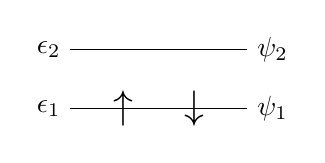
\begin{tikzpicture}[scale=1.5]
		\draw (0,0)node[left]{$\epsilon_1$} --node[pos=.3]{\Large$\uparrow$}node[pos=.7]{\Large$\downarrow$}+(1.5,0)node[right]{$\psi_1$};
		\draw (0,.5)node[left]{$\epsilon_2$}--node[pos=.3]{}node[pos=.7]{}+(1.5,0)node[right]{$\psi_2$};
	\end{tikzpicture}
\end{figure}
可以通过观察直接写出总能. 
两个电子中每个都对应动能加上核吸引势能$h_{11}=(\psi_1|h|\psi_1)$, 
此外还有两电子间的库伦排斥$J_{11}=(\psi_1\psi_1|\psi_1\psi_1)$. 
这里没有交换作用, 
因为两电子的自旋反平行. 
那么\hft 能量就是
\begin{align}
	E_0 = 2h_{11} + J_{11}
\end{align}
这与\autoref{3.127}相符, 
因为$J_{ii}=K_{ii}$.


可按同样的方式计算轨道能量
\begin{figure}[H]\centering
	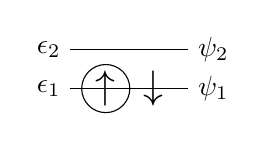
\begin{tikzpicture}
		\draw (0,0)node[left]{$\epsilon_1$} --node[inner sep=1,shape=circle,draw,pos=.3]{\Large$\uparrow$}node[pos=.7]{\Large$\downarrow$}+(1.5,0)node[right]{$\psi_1$};
		\draw (0,.5)node[left]{$\epsilon_2$}--node[pos=.3]{}node[pos=.7]{}+(1.5,0)node[right]{$\psi_2$};
	\end{tikzpicture}
\end{figure}
要计算$\epsilon_c$, 
将圆圈内的电子的作用加起来即得. 
有动能和核吸引势能$h_{11}$, 
以及库伦作用$J_{11}$, 
那么
\begin{align}
	\epsilon_1 = h_{11} + J_{11}
\end{align}
方法适用于任何占据轨道的能量. 
对于虚轨道, 
如之前所看到的, 
轨道能量对应于额外的第$(N+1)$个电子的作用, 
这与Koopmans定理相符. 
在这里的极小基模型中, 
需保持$\ket{\Psi_0}$中的两个电子不动, 
然后计算虚轨道上一个外来电子的能量, 
如图所示
\begin{align}
	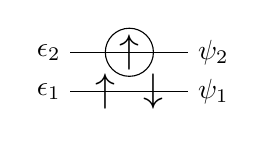
\begin{tikzpicture}
		\draw (0,0)node[left]{$\epsilon_1$} --node[pos=.3]{\Large$\uparrow$}node[pos=.7]{\Large$\downarrow$}+(1.5,0)node[right]{$\psi_1$};
		\draw (0,.5)node[left]{$\epsilon_2$}--node[inner sep=1,shape=circle,draw,pos=.5]{\Large$\uparrow$}node[pos=.7]{}+(1.5,0)node[right]{$\psi_2$};
	\end{tikzpicture}
\end{align}
圈内电子有动能加核吸引势能$h_{22}$, 
并与其他两个电子分别有库伦作用$J_{12}$, 
再加上与同自旋电子的一个交换作用$-K_{12}$. 
因此
\begin{align}
	\epsilon_2 = h_{22} + 2J_{12} - K_{12}
\end{align}

以上两个结果与练习3.9中闭壳层轨道能量的一般表达式相符.

\subsection{引入基函数:Roothaan方程}
因为我们已经消掉了自旋, 
那么分子轨道计算就等价于求解如下的积分微分方程
\begin{align}
	\label{3.132}
	f(\bfr_r)\psi_i(\bfr_1) = \epsilon_i\psi_i(\bfr_1)
\end{align}
也许你会尝试数值求解该方程, 数值解在原子的计算中十分普遍, 但目前确实没有可行的办法得到分子的数值解. 
Roothaan\endnote{
	C. C. J. Roothaan, New Development in molecular prbital theory, \textit{Rev. Mod. Phys.} \textbf{23:} 69 (1951).
}
的贡献就是证明了通过引入一组已知的空间基函数, 该微分方程可以转化为一组代数方程并可用标准的矩阵技术来求解.

那么我们就引入一组$K$个已知的基函数$\{\phi_\mu(\bfr)|\mu=1,2,\ldots,K\}$并将未知的分子轨道线性展开:
\begin{align}
	\label{3.133}
	\psi_i = \sum_{\mu=1}^{K}C_{\mu i}\phi_\mu\quad i = 1,2,\ldots,K
\end{align}
若集合$\{\phi_\mu\}$完备, 
那么该展开就是精确的, 
而且任意一组完备集$\{\phi_\mu\}$都可用于展开. 
但是事与愿违, 
由于实际计算中的原因, 
我们只能使用有限$K$个基函数. 
正因如此, 
选择一个尽可能精确地展开分子轨道的基组就非常重要, 
尤其是对于$\ket{\Psi_0}$中被占分子轨道$\{\psi_a\}$(由它们来确定基态能量$E_0$)的展开. 
本章后一阶会讨论基组选择的问题并讲述一点选择基组的艺术. 
就我们当下的目的来看, 
只需预设$\{\phi_\mu\}$是一组已知的函数就行. 
当基组越来越完备时, 
展开\autoref{3.133}就可以越来越准确地表示“精确”的分子轨道, 
也就是(近似)的分子轨道 收敛到了\autoref{3.132}中的(精确)分子轨道——Fock算符的真实本征函数. 
对任意的有限基组. 
我们所得的分子轨道都是截断的展开\autoref{3.133}, 
它仅仅精确到由$\{\phi_\mu\}$所张的空间(即在仅这个子空间内是精确的).


由\autoref{3.133}可知, 
计算\hft 分子轨道的问题约化为计算一组展开系数$\{C_{\mu i} \}$的问题. 
我们可将线性展开\autoref{3.133}带入\hft 方程\autoref{3.132}得到一个矩阵方程. 
若使用指标$\nu$, 
则方程为
\begin{align}
	f(1) \sum_\nu C_{\nu i}\phi_\nu(1) = \epsilon_i\sum_\nu C_{\nu i}\phi_\nu(1) 
\end{align}
左乘$\phi_\mu^*(1)$并积分, 
就将这个积分微分方程转化为矩阵方程
\begin{align}
	\label{3.135}
	\sum_\nu C_{\nu i}\int\dd{r}_1\,\phi_\nu^*(1)f(1)\phi_\nu(1) = \epsilon_i\sum_\nu C_{\nu i}\int\dd{r}_1\,\phi_\nu^*(1)\phi_\nu(1)
\end{align}

现在定义两个矩阵:

1. \emph{重叠矩阵$\mathbf{S}$}的矩阵元为
\begin{align}
	\label{3.136}
	S_{\mu\nu}=\int\dd{r}_1\,\phi_\mu^*(1)\phi_\nu(1)
\end{align}
该矩阵为$K\times K$厄米矩阵(虽然通常是实对称阵). 
虽然假设基函数$\{\phi_\mu\}$为归一化且相互线性独立, 
但它们一般不相互正交, 
因此就互有重叠, 
重叠大小为$0\leqslant|S_{\mu\nu}|\leqslant1$, 
即$\mathbf{S}$的对角元为$1$非对角元的绝对值都小于$1$. 
非对角元的符号取决于两个基函数的相对符号、相对取向及在空间上的分离程度. 
若两个非对角元趋近于$1$(按绝对值), 
即趋近于完全重叠, 
那么两个基函数就趋近线性相关. 
由于重叠矩阵为厄米的, 
它可被一个酉矩阵对角化, 
之后我们会来做这件事. 
重叠矩阵的本征值可以证明一定是正数, 
因此重叠矩阵是正定矩阵. 
基组中的线性相关与重叠矩阵中趋于零的本征值相联系. 
重叠矩阵有时也叫作度规矩阵(metric matrix). 


2. \emph{Fock矩阵$\mathbf{F}$}的矩阵元为
\begin{align}
	F_{\mu\nu} = \int\dd{r}_1\,\phi_\mu^*(1)f(1)\phi_\nu(1)
\end{align}
它也是$K\times K$的厄米矩阵(虽然常为实对称阵). 
Fock算符$f(1)$是单电子算符, 
任意一组单电子函数即定义该算符的一种矩阵表示. 
之前已讨论过Fock算符在自旋轨道下的矩阵元. 
Fock矩阵$\mathbf{F}$就是Fock算符在一组基函数$\{\phi_\mu\}$下的矩阵表示.


有了$\mathbf{F,S}$的定义, 
就可将积分形式的\hft 方程\autoref{3.135}写为
\begin{align}
	\sum_\nu F_{\mu\nu} C_{\nu i} = \epsilon_i\sum_{\nu}S_{\mu\nu}C_{\nu i}\quad i=1,2,\ldots,K
\end{align}
这组方程就是\emph{Roothaan方程}, 
可以写成更紧凑的单个矩阵方程:
\begin{align}
	\label{3.139}
	\mathbf{FC=SC}\bm{\epsilon}
\end{align}
式中$\mathbf{C}$是展开系数$C_{\mu i}$构成的$K\times K$方阵:
\begin{align}
	\label{3.140}
	\mathbf{C} =
	\begin{pmatrix}
		C_{11} & C_{12} & \cdots & C_{1K} \\
		C_{21} & C_{22} & \cdots & C_{2K} \\
		\vdots & \vdots &        & \vdots \\
		C_{K1} & C_{K2} & \cdots & C_{KK}
	\end{pmatrix}
\end{align} 
$\bm{\epsilon}$是轨道能量$\epsilon_i$构成的对角阵:
\begin{align}
	\label{3.141}
	\bm{\epsilon} = 
	\begin{pmatrix}
		\epsilon_1 &            &        &            \\
		& \epsilon_2 &        & \mathbf{0} \\
		\mathbf{0} &            & \ddots &            \\
		&            &        & \epsilon_K
	\end{pmatrix}
\end{align}
需注意\autoref{3.133}到\autoref{3.140}中, 
由$\mathbf{C}$的列来描述分子轨道, 
也即描述$\psi_1$的系数是$\mathbf{C}$的第一列, 
描述$\psi_2$的系数是$\mathbf{C}$的第二列, 
等等.

\exercise{
	请证明$\mathbf{C^\dagger SC=1}$. 
	\textit{提示:}分子轨道$\{\psi_i\}$是正交的.
	
}
到此确定\hft 分子轨道$\{\psi_i\}$和轨道能量$\epsilon_i$的问题就与求解矩阵方程$\mathbf{FC=SC}\bm{\epsilon}$关联在一起. 
要想更进一步, 
需将Fock矩阵的显式表达式写出来. 
但我们必须先来介绍密度矩阵的概念.


\subsection{电荷密度}
若某电子由空间波函数$\psi_a(\bfr)$描述, 
那么在点$\bfr$附近以小体积元$\dd{r}$内找到该电子的概率就是$|\psi_a(\bfr)|^2\dd{r}$. 
这个概率分布函数(电荷密度)就是$|\psi_a(\bfr)|^2$. 
若由一个闭壳层分子, 
由一单行列式所描述, 
每个被占分子轨道上都有两个电子, 
那么总的电荷密度就是
\begin{align}
	\label{3.142}
	\rho(\bfr) = 2 \sum_{a}^{N/2} |\psi_a(\bfr)|^2
\end{align}
因此$\rho(\bfr)\dd{r}$就是找到一个电子在$\bfr$出的$\dd{r}$内的概率. 
对电荷密度积分就得总电子数:
\begin{align}
	\int\dd{r}\rho(\bfr) = 2 \sum_{a}^{N/2} \int\dd{r}|\psi_a(\bfr)|^2 = 2\sum_{a}^{N/2}1=N
\end{align}
对于单行列式, 
这些方程就说明总电荷密度就是各个电子的电荷密度之和.

\exercise{
	使用密度算符$\hat{\rho}(\bfr)=\sum_{i=1}^{N}\delta(\bfr_i-\bfr)$、第二章中求矩阵元的规则, 
	以及自旋轨道到空间轨道的转换规则, 
	由$\rho(\bfr)=\braket{\Psi_0|\hat{\rho}(\bfr)|\Psi_0}$推得\autoref{3.142}.
	
}

现在把分子轨道展开\autoref{3.133}插入\autoref{3.142}得到电荷密度:
\begin{align}
	\rho(\bfr) & = 2\sum_{a}^{N/2}\psi_a^*(\bfr)\psi_a(\bfr) \notag\\
	& = 2\sum_{a}^{N/2}\sum_{v} C_{\nu a}^*\phi_\nu^*(\bfr)\sum_{\mu}C_{\mu a}\phi_\mu(\bfr) \notag\\
	& = \sum_{\mu\nu}\left[ 2\sum_{a}^{N/2}C_{\mu a}C_{\nu a}^* \right]\phi_\mu(\bfr)\phi_\nu(\bfr) \notag\\
	& = \sum_{\mu\nu}P_{\mu\nu} \phi_\mu(\bfr)\phi_\nu(\bfr)
	\label{3.144}
\end{align}

其中我们定义了\emph{密度矩阵},
或者用另一个名字, 
\emph{电荷密度键级矩阵}:
\begin{align}
	P_{\mu\nu} = 2\sum_{a}^{N/2}C_{\mu a}C_{\nu a}^*
	\label{3.145}
\end{align}
由\autoref{3.144}知,
给定一组已知的基函数$\{\phi_\mu\}$, 
矩阵$\mathbf{P}$就完全确定了电荷密度$\rho(\bfr)$. 
它通过\autoref{3.145}和展开系数$\mathbf{C}$直接联系起来,
那么我们就能用$C_{\mu i}$或$P_{\mu\nu}$来表示闭壳层\hft 的计算结果。


\exercise{
	矩阵$\mathbf{A}$ 若满足$\mathbf{A}^2=\mathbf{A}$, 
	我们就称其为等幂的. 
	使用练习3.
	10的结果,
	证明$\mathbf{PSP}=2\mathbf{P}$, 
	也即,
	证明$\frac{1}{2}\mathbf{P}$在正交归一基下是等幂的。
	
	\Next
	用\autoref{3.122}的闭壳层Fock算符表达式证明
	\begin{align}
		\label{3.146}
		f(\bfr_1) & = h(\bfr_1) + v^\mathrm{HF}(\bfr_1)\notag\\
		& = h(\bfr_1) + \frac{1}{2}\sum_{\lambda\sigma}P_{\lambda\sigma}\left[ \int\dd{r}_1\,\phi_\sigma^*(\bfr_2)(2-\scr{P}_{12})\twoe\phi_\lambda(\bfr_2)\right]
	\end{align}
}
上面练习的结果用密度矩阵表示了Fock算符. 
可用此表达式从直觉上来说明\hft 手续怎样进行. 
我们先猜一个密度矩阵$\mathbf{P}$, 
也即猜一个描述电子位置的电荷密度$\rho(\bfr)$. 
之后会有一些内容介绍如何猜. 
然后使用猜测的电荷密度根据\autoref{3.146}计算电子的有效单电子势$v^\mathrm{HF}(\bfr_1)$. 
由此就得到有效单电子\ha (Fock算符), 
然后就可求解单电子的类\sch 方程以确定有效势中的单电子态$\{\psi_i\}$. 
由\autoref{3.142}可用新的单电子态(即分子轨道$\{\psi_i\}$)确定对密度的更优近似. 
有了新的电荷密度就能计算新的\hft 势,然后重复以上手续直到\hft 势不再改变(有效静电场也随之不再改变), 
也即, 
直到(通过求解类\sch 方程)产生电荷密度的场与前一次的场(及\hft 本征值方程)相洽(相同)(使用\autoref{3.146}). 
这就是\hft 方程常叫作\emph{自洽场}方程的缘故. 
这也是看待求解Roothaan方程所涉及物理的一种视角. 
回到真实的代数手续中, 
需将Fock矩阵的$\mathbf{F}$的显式表达式给出.

\subsection{Fock矩阵的表达式}
Fock矩阵$\mathbf{F}$是Fock算符
\begin{align}
	f(1) = h(1) + \sum_{a}^{N/2}2J_a(1) -K_a(1)
\end{align}
在基$\{\phi_\mu\}$下的矩阵表示
\begin{align}
	\label{3.148}
	F_{\mu\nu} & = \int\dd{r}_1\,\phi_\mu^*(1)f(1)\phi_\nu(1)\notag\\
	& = \int\dd{r}_1\,\phi_\mu^*(1)h(1)\phi_\nu(1) + \sum_{a}^{N/2}\int\dd{r}_1\,\phi_\mu^*(1)[2J_a(1)-K_a(1)]\phi_\nu(1)\notag\\
	& = H_{\mu\nu}^\mathrm{core} + \sum_{a}^{N/2}2(\mu\nu|aa)-(\mu a|a\nu)
\end{align}
式中定义了\emph{核\ha}矩阵
\begin{align}
	H_{\mu\nu}^\mathrm{core} = \int\dd{r}_1\,\phi_\mu^*(1)h(1)\phi_\nu(1)
\end{align}
核\ha 矩阵中的元素是含单电子算符$h(1)$的积分, 
由它描述一个电子的动能及核吸引势能:
\begin{align}
	h(1) = -\frac{1}{2}\nabla_1^2 - \sum_A\frac{Z_A}{|\mathbf{r}_1-\mathbf{R}_A|}
\end{align}

计算核\ha 矩阵元涉及到求动能积分:
\begin{align}
	T_{\mu\nu}\int\dd{r}_1\,\phi_\mu^*(1)[-\frac{1}{2}\nabla_1^2]\phi_\nu(1)
\end{align}
以及核吸引积分:
\begin{align}
	V_{\mu\nu}^\mathrm{nucl} = \int\dd{r}_1\,\phi_\mu^*(1)\left[ -\sum_{A}\frac{Z_A}{|\mathbf{r}_1-\mathbf{R}_A|} \right]\phi_\nu(1)
\end{align}
那么
\begin{align}
	H_{\mu\nu}^\mathrm{core} = T_{\mu\nu} + V_{\mu\nu}^\mathrm{nucl}
\end{align}
在具体的基组$\{\phi_\mu\}$下, 
$\mathbf{T,V^\mathrm{nucl}}$中的积分会具体地计算出来, 
有一构成核\ha 矩阵. 
核\ha 矩阵与Fock矩阵不同, 
在迭代计算的过程中只需被计算一次, 
然后保持不变. 
动能核核吸引积分的计算会在附录A讲述.


回到\autoref{3.148}的Fock矩阵表达式, 
现要将分子轨道展开\autoref{3.133}插入到双电子项中, 
得到
\begin{align}
	\label{3.154}
	F_{\mu\nu} & = H_{\mu\nu}^\mathrm{core} + \sum_{a}^{N/2}\sum_{\lambda\sigma}C_{\lambda a}C^*_{\sigma a}[2(\mu\nu|\sigma\lambda)-(\mu\lambda|\sigma\nu )]\notag\\
	& = H_{\mu\nu}^\mathrm{core} + \sum_{\lambda\sigma}P_{\lambda\sigma}[(\mu\nu|\sigma\lambda)-\frac{1}{2}(\mu\lambda|\sigma\nu )]\notag\\
	& = H_{\mu\nu}^\mathrm{core} + G_{\mu\nu}
\end{align}
式中$G_{\mu\nu}$是Fock矩阵的双电子部分. 
这就是Fock矩阵的最终表达式. 
它包含单电子部分$\mathbf{H}^\mathrm{core}$, 
这部分在给定基组下保持不变, 
还包括双电子部分$\mathbf{G}$, 
它依赖密度矩阵$\mathbf{P}$及一组双电子积分:
\begin{align}
	(\mu\nu|\lambda\sigma) = \int\dd{r}_2\,\phi_\mu^*(1)\phi_\nu(1)\twoe\phi_\lambda^*(2)\phi_\sigma(2)
\end{align}
由于双电子积分数目较多, 
所以\hft 计算中的主要困难就是操作、计算这些双电子积分.

\exercise{
	若基函数为实的, 
	请用双电子积分的对称性$[(\mu\nu|\lambda\sigma)=(\nu\mu|\lambda\sigma)=(\lambda\sigma|\mu\nu)]$
	证明含$K=100$个基函数的基组有$12753775=O(K^4/8)$个互不相同的双电子积分.
}

由于Fock矩阵依赖密度矩阵
\begin{align}
	\mathbf{F=F(P)}
\end{align}
或者等价地, 
依赖于展开系数
\begin{align}
	\mathbf{F=F(C)}
\end{align}
因此Roothaan方程是非线性的, 
即
\begin{align}
	\mathbf{F(C)C=SC}\bm{\epsilon}
\end{align}
所以需要迭代求解. 
考虑如何进行迭代之前, 
现讨论如下矩阵方程的在每步迭代中的解
\begin{align}
	\mathbf{FC=SC}\bm{\epsilon}
\end{align}
若$\mathbf{S}$是单位阵(即若基组是正交归一的)那么就有
\begin{align}
	\mathbf{FC=C}\bm{\epsilon}
\end{align}
Roothaan方程就成为通常本征值方程的形式, 
然后将$\mathbf{F}$对角化即可求出本征矢$\mathbf{C}$和本征值$\bm{\epsilon}$. 由于当下的基组不正交,需对本征值问题$\mathbf{FC=SC}\bm{\epsilon}$进行重构.
\subsection{基的正交归一化}
分子的计算中所使用的基组是非正交归一基. 
基函数确实是归一的, 
单它们之间不正交. 
这就产生了Roothaan方程中的重叠矩阵. 
为将Roothaan写为通常的矩阵本征值问题, 
需要正交化基函数.


若有一组函数$\{\phi_\mu\}$非正交, 
也即
\begin{align}
	\int\dd{r}\phi_\mu^*(\bfr)\phi_\nu(\bfr) = S_{\mu\nu}
\end{align}
则总能够找到一个变换矩阵(非酉矩阵)使得变换后的函数集合$\{\phi_\mu'\}$
\begin{align}\label{3.162}
	\phi_\mu' = \sum_{\nu}X_{\nu\mu}\phi_\nu
\end{align}
构成一个正交归一集:
\begin{align}
	\label{3.163}
	\int\dd{r}\phi_\mu^{\prime*}(\bfr)\phi_\nu'(\bfr) = \delta_{\mu\nu}
\end{align}
为得到$\mathbf{X}$的具体性质, 
我们将变换\autoref{3.162}带入\autoref{3.163}得到
\begin{align}
	\int\dd{r}\phi_\mu^{\prime *}(\bfr)\phi_\nu^{\prime}(\bfr) & = \int\dd{r}\left[ \sum_{\lambda}X_{\lambda\mu}^*\phi_{\lambda}^*(\bfr)\right]\left[ \sum_\sigma X_{\sigma\nu}\phi_\sigma(\bfr) \right]\notag\\
	& = \sum_\lambda\sum_\sigma X_{\lambda\sigma}^*\int\dd{r}\phi_\lambda^*(\bfr)\phi_\sigma(\bfr)X_{\sigma\nu}\notag\\
	& = \sum_\lambda\sum_\sigma X_{\lambda\mu}^*S_{\lambda\sigma}X_{\sigma\nu} = \delta_{\mu\nu}
\end{align}
最后的等式可写为矩阵方程
\begin{align}\label{3.165}
	\mathbf{X^\dagger SX}=1
\end{align}
如果变换后的轨道构成正交归一集, 
上式就是$\mathbf{X}$必须满足的关系. 
我们之后会知道, 
$\mathbf{X}$必须是非奇异的, 
也即它必须有逆矩阵$\mathbf{X}^{-1}$. 
当前我们先来看如何得到两个不同的变换矩阵$\mathbf{X}$. 
由于$\mathbf{S}$是厄米的, 
所以可用酉矩阵$\mathbf{U}$将其对角化:
\begin{align}
	\mathbf{U^\dagger SU=s}
\end{align} 
其中$\mathbf{s}$是$\mathbf{S}$本征值构成的对角阵.

\exercise{
	使用定义$S_{\mu\nu}=\int\dd{r}\phi_\mu^*\phi_\nu$证明$\mathbf{S}$的本征值全为正数. 
	\textit{提示:}考虑$\sum_\nu S_{\mu\nu}c_\nu^i=s_ic_\mu^i$, 
	乘以$c_\mu^{i*}$并求和, 
	这里$\mathbf{c}^i$是$\mathbf{U}$的第$i$行.
	
}

一般用到的基组$\{\phi_\mu\}$正交化方案有两种. 一种是\emph{对称正交化}, $\mathbf{X}$就是$\mathbf{S}$的负平方根:
\begin{align}\label{3.167}
	\mathbf{X} = \mathbf{S}^{-1/2} = \mathbf{U}\mathbf{s}^{-1/2}\mathbf{U}^\dagger
\end{align}
回忆第一章对矩阵函数的讨论, 
我们可以如此构建$\mathbf{S}^{-1/2}$:将$\mathbf{S}$对角化为$\mathbf{s}$, 
取每个本征值的负平方根, 
构成一个对角阵$\mathbf{s}^{-1/2}$, 
然后用\autoref{3.167}中的变换``逆对角化”. 
若$\mathbf{S}$厄米, 
则$\mathbf{S}^{-1/2}$也厄米. 
将\autoref{3.167}带入\autoref{3.165}
\begin{align}
	\mathbf{S}^{-1/2}\mathbf{SS}^{-1/2} = \mathbf{S}^{-1/2}\mathbf{S}^{1/2} = \mathbf{S}^0 = \mathbf{1}
\end{align} 
可以看到$\mathbf{X=S}^{-1/2}$确实为一个正交化变换矩阵. 
由于$\mathbf{S}$的本征值都为正(练习3.5), 
所以\autoref{3.167}中开平方的操作没有问题. 
但是若基组中出现线性相关或这近线性相关, 
则某些本征值将接近零, 
\autoref{3.167}中某些除数会接近零. 
因此对称正交化会因近线性相关发生数值精度上的问题.


第二种正交化基组的方案叫作\emph{正则正交化}. 
它使用的变换矩阵如下
\begin{align}
	\mathbf{X=Us}^{-1/2}
\end{align}
这就是说, 
酉矩阵$\mathbf{U}$中的行要除以对应本征值的平方根:
\begin{align}
	X_{ij} = U_{ij}/s_{j}^{1/2}
\end{align}
将$\mathbf{X}$的定义\autoref{3.165}带入, 
可得
\begin{align}
	\mathbf{X^\dagger SX} = (\mathbf{Us}^{-1/2})^\dagger\mathbf{SUs}^{-1/2} = \mathbf{s}^{-1/2}\mathbf{U^\dagger SUs}^{-1/2} = \mathbf{s}^{-1/2}\mathbf{ss}^{-1/2}=\mathbf{1}
\end{align}
这就证明$\mathbf{X=Us}^{-1/2}$也是一正交化变换矩阵. 
从(3.170)可以看到, 
若基组中存在(近)线性相关(即某些本征值$s_i$接近零.
), 
则正交化手续会引发困难. 
但用正则正交化即可规避这种难处. 
在矩阵本征值问题(3.166)中, 
可以将对角阵$\mathbf{s}$中的本征值按任意顺序排列, 
只要将$\mathbf{U}$中的列也以相同方式放置即可. 
设想按该顺序排列本征值:$s_1>s_2>s_3>\cdots$. 
若观察发现最后的$m$个值太小, 
将发数值问题, 
那么将如下的截断矩阵$\mathbf{\tilde{X}}$作为变换矩阵:
\begin{align}
	\tilde{\mathbf{X}} =
	\begin{pmatrix}
		U_{1,1}/s^{1/2}_{1} & U_{1,2}/s^{1/2}_{2} & \cdots & U_{1,K-m}/s^{1/2}_{K-m} &  \\
		U_{2,1}/s^{1/2}_{1} & U_{2,2}/s^{1/2}_{2} & \cdots & U_{2,K-m}/s^{1/2}_{K-m} &  \\
		\vdots              & \vdots              &        & \vdots                  &  \\
		U_{K,1}/s^{1/2}_{1} & U_{K,2}/s^{1/2}_{2} & \cdots & U_{K,K-m}/s^{1/2}_{K-m} &
	\end{pmatrix}
\end{align}
其中我们去掉了$\mathbf{X}$的后$m$列, 
得到$K\times (K-m)$矩阵$\tilde{\mathbf{X}}$. 
用这个截断的变换矩阵, 
变换后仅能得到$K-m$个正交归一基函数:
\begin{align}
	\phi_\mu' = \sum_{\nu=1}^{K}\tilde{X}_{\nu\mu}\phi_\nu\quad\mu=1,2,\ldots,K-m
\end{align}
若我们去掉的本征值真的为零, 
则以上函数所张的空间与原先函数所张的空间完全相同. 
实际中碰到线性相关问题时本征值的大小通常是$s_i\leqslant 10^{-4}$(这个区间当然依赖于计算时的机器精度). 
去掉的列及本征值就意味着``扔掉''了一部分基组, 
但也仅是很小一部分而已.


处理非正交基组的手段之一是将函数${\phi_\mu}$正交化, 
得到变换后的基函数$\phi_\mu'$并在之后一直使用变换后的函数. 
这种办法消掉了Roothaan方程中的重叠矩阵$\mathbf{S}$. 
后面求解时只需对角化Fock矩阵. 
但这意味着必须用新轨道计算所有的双电子积分, 
或者将旧双电子积分$(\mu\nu|\lambda\sigma)$变换为新的$(\mu'\nu'|\lambda'\sigma')$. 
实际上这非常耗时. 
我们可用更高效的办法处理该问题. 
考虑新的系数矩阵$\mathbf{C}'$, 
它与旧系数矩阵的关系为
\begin{align}
	\mathbf{C'=X}^{-1}\mathbf{C}\quad \mathbf{C=XC'}
\end{align}
此处假设$\mathbf{X}$有逆矩阵. 
消掉线性相关后这肯定成立. 
将$\mathbf{C=XC'}$带入Roothaan方程得到
\begin{align}
	\mathbf{FXC'=SXC'}\bm{\epsilon}
\end{align} 
左乘$\mathbf{X^\dagger}$得
\begin{align}
	(\mathbf{X^\dagger FX}\mathbf{C'}) = (\mathbf{X^\dagger SX})\mathbf{C'}\bm{\epsilon}
\end{align}
若定义新矩阵$\mathbf{F}'$为
\begin{align}
	\mathbf{F'=X^\dagger FX}
\end{align}
并用(3.165), 
那么
\begin{align}
	\mathbf{F'C'=C'}\bm{\epsilon}
\end{align}
这就是变换后的Roothaan方程, 
可将$\mathbf{F'}$对角化以解得$\mathbf{C'}$. 
有了$\mathbf{C'}$, 
$\mathbf{C}$就能从(3.174)得到. 
因此给定$\mathbf{F}$, 
可用(3.177)(3.178)(3.174)求解Roothaan方程$\mathbf{FC=SC}\bm{\epsilon}$. 
中间的带撇矩阵就是正交基下的Fock矩阵和展开系数:
\begin{align}
	\psi_i & = \sum_{\mu=1}^{K}C_{\mu i}'\phi_\mu'\\
	F_{\mu\nu}' & = \int\dd{r}_1\,\phi^{\prime*}_\mu(1)f(1)\phi_\nu'(1)
\end{align}
\exercise{
	用(3.179)(3.180)(3.162)导出(3.174)(3.177).
	
}
\subsection{SCF(自洽场)流程}
有了前面几节的背景知识, 
现在是时候介绍如何得到分子限制性波函数(即$\ket{\Psi_0}$)的实际计算流程了. 
有些作者认为\hft 解这个术语只能在\hft 极限下使用, 
此时基组是完备的, 
他们用自洽场解来称呼在有限基组(基组可能很小)下的解. 
但我们会混合使用\hft 和自洽场(SCF)这两个术语, 
如有需要, 
才会特别指出是否在\hft 极限下. 
SCF流程如下:
\begin{enumerate}[1.]
	\item 确定一个分子(一组核坐标$\{\mathbf{R}_A\}$, 原子序数$Z_A$, 电子数$N$)和基组$\{\phi_A\}$.
	\item 计算所需的分子积分, $S_{\mu\nu},H_{\mu\nu}^\mathrm{core}, (\mu\nu|\lambda\sigma)$.
	\item 对角化重叠矩阵$\mathbf{S}$, 用(3.167)或(3.169)得到变换矩阵$\mathbf{X}$.
	\item 猜测一个密度矩阵$\mathbf{P}$.
	\item 用密度矩阵$\mathbf{P}$计算(3.154)中的矩阵$\mathbf{G}$和双电子积分$(\mu\nu|\lambda\sigma)$.
	\item $\mathbf{G}$加核\ha 矩阵得到Fock矩阵$\mathbf{F=H}^\mathrm{core}+\mathbf{G}$.
	\item 计算变换后的Fock矩阵$\mathbf{F'=X^\dagger FX}$.
	\item 对角化$\mathbf{F'}$得到$\mathbf{C'},\bm{\epsilon}$.
	\item 根据(3.14)用$\mathbf{C}$构建新密度矩阵$\mathbf{P}$.
	\item 确定该过程是否收敛, 即确定(10)中密度矩阵是否与前一个密度矩阵在某种判据下相同. 若未收敛, 回到(5)用新密度矩阵计算.
	\item 若收敛, 则用得到的解表示出$\mathbf{C,P,F}$等, 即计算期望值和其他想求的量.
\end{enumerate}
之后会期望值(如能量、偶极矩等)及其他有用的量(如布居分析)的计算方法(3.4.7节). 
但我们先来考察执行以上十二个步骤时的一些实际问题.


在Born-Oppenheimer近似中, 
以上步骤所做的就是确定处在$M$个点电荷($M$个带电荷为$Z_A$的核)中的$N$个电子的波函数$\ket{\Psi_0}$(也就确定了能量$E_0$). 
有了电子能量, 
再加上经典的核-核排斥能即得到以核坐标$\{\mathbf{R}_A\}$为变量的总能函数. 
在不同 的核坐标下重复计算步骤, 
就能研究核运动的核势能面. 
一类常见的计算是在能量最低的核坐标$\{\mathbf{R}_A\}$下进行, 
这就是分子平衡构型下的计算. 
以上手续对任何一组点电荷都有效. 
具体地, 
比如``超分子''(supermolecule)计算就是用大于一个分子集体的核电荷坐标, 
这常见于研究分子间力的情形.


选定一组核坐标后, 
限制性闭壳层单行列式波函数就由一组基函数$\{\phi_\mu\}$所完全确定. 
因此这就是所谓\emph{从头算}的一例, 
这种计算中对积分与电子\ha 不作近似, 
结果完全由基组与核坐标确定. 
选择基组更像一种艺术而非科学. 
很明显, 
计算机设备、预算等会将限制我们的选择——通常是有限个基函数组成的较小基组. 
因此选择基组必须要审慎. 
当前通用的只有Slater型和Gaussian型函数. 
若对每个原子用的函数组较小, 
那么Slater型函数会给出很好的能量. 
当每个原子配备的函数个数增大时, 
Slater函数的明显优势会被抹平. 
除了基组所张函数空间大小外, 
实际过程中还要考虑计算分子积分的时间. 
多数多原子计算会用Gaussian轨道, 
因为用这种函数计算积分的速度可以显式地知道, 
本书会着重于Gaussian基函数. 
基函数在本章3.6节讨论, 
3.5.1节讨论$1s$ STO-3G基, 
在将其用于$\hd$和$\mathrm{HeH}^+$的模型计算前.


选定基组后, 
就要计算并储存很多不同类型的积分. 
附录A中介绍了Gaussian基函数的分子积分计算, 
此处我们仅提及一小部分相关知识. 
后面一点会讲述计算核\ha 及单电子期望值所用的重叠积分与单电子积分, 
这部分与双电子积分比起来相对简单, 
主要是由于单电子积分数目较少. 
大一些的计算中主要困难是计算核操作巨量双电子积分. 
若有$K$个基函数, 
就有约$K^4/8$个互不相同的双电子积分. 
中性分子的小基组计算中双电子积分很容易超过几百万个. 
不过问题还不是很严重, 
因为大分子中当基函数间的距离比较大时, 
很多积分基本上为零. 
分子对称性又会使一大批积分为零. 
但是双电子积分还是太多, 
没办法都存入计算机内存. 
常见的做法是将非零积分按随机顺序存入外部磁盘或磁带, 
每个积分都附带一个标签以表明指标$\mu,\nu,\lambda,\sigma$.


后一节中会介绍两种正交化基组(或者说求$\mathbf{X}$)的方式, 
如此就可用对角化的办法求解Roothaan方程. 
若取$\mathbf{X=S}^{1/2}$, 
则概念简单, 
仅在非一般的情况下(基组中的线性相关情况严重)才会用到正则正交化. 
正则正交化中会去掉$\mathbf{X=Us}^{1/2}$中的一些列, 
如此就得到一长方阵. 
若$\mathbf{X}$中有$m$列被去掉, 
那么相当于使用$K-m$大小的基组, 
因此会得到$K-m$个分子轨道$\psi_i$, 
也即$\mathbf{F'}$为$(K-m)\times(K-m)$矩阵, 
$\mathbf{C'}$是$K\times(K-m)$矩阵, 
其列在原始的$K$个基函数下描述$K-m$个分子轨道.


对密度矩阵$\mathbf{P}$最简单的可能猜测是零矩阵. 
这相当于将$\mathbf{F}$近似为$\mathbf{H}^\mathrm{core}$, 
并在首次迭代中忽略所有电子-电子相互作用. 
用这种方式可以非常方便地开始迭代手续. 
它对应的是将收敛分子轨道用核势场中单电子的轨道来近似. 
但是$N$-电子分子的分子轨道可能与对应单电子分子的轨道非常不同, 
用核\ha 作为Fock矩阵的初猜时SCF手续经常不收敛. 
半经验的扩展H\"uckel计算会产生一个``有效''$\mathbf{F}$, 
常用它来作为波函数的初猜, 
这种猜测的效果比用核\ha 要好. 
此外还有很多其他方式可以生成初猜.


实际迭代手续中最耗时的部分是把双电子积分和密度矩阵乘起来得到矩阵$\mathbf{G}$(第(5)步). 
若积分按照随机顺序存入外部储存器, 
且每个都带有指示标签, 
那么之后当积分读入主储存时, 
可以用标签也就是指标$\mu,\nu,\lambda,\sigma$来指认积分, 
然后确定要对密度矩阵中哪些元素做乘法, 
并按照(3.154)中$\mathbf{G}$矩阵的表达式, 
确定$\mathbf{G}$矩阵中哪个元素需要加上乘出来的乘积.


多数计算中, 
如果使用比较高效的对角化手续, 
步骤(6)(10)的矩阵操作不会太费时(相较于构建$\mathbf{G}$矩阵).


由于Roothaan方程是非线性方程, 
这里讲的简单迭代手续往往不会收敛. 
若初猜质量较差, 
可能出现振荡或发散. 
若是振荡, 
将前后密度矩阵作平均可能有效. 
即使能收敛,收敛过程有时也较慢. 
利用两个及以上相邻的密度矩阵, 
可以设计出许多外推手续. 
收敛问题不是一个平凡问题, 
它是很多计算中的头号问题. 
本书讲的迭代手续也许可以尝试的最简单的一种, 
但它确实有些过于简单. 
现在已有许多其他的技术来确保或加速SCF解的收敛.


当然, 
我们需要一个是否收敛的判据, 
比较常用的办法就是简单地观察每一步的总电子能量, 
要求两个相邻步骤的值只差一个小量$\delta$. 
$\delta=10^{-6}$Hartrees在多数情况下就够用了. 
等一下我们会马上证明, 
每次迭代中计算一下能量几乎不需要花费时间. 
另外一种判据是, 
要求密度矩阵的矩阵元前后的标准偏差, 
即下式
\begin{align*}
	\left[ K^{-2}\sum_\mu\sum_\nu[P{(i)}_{\mu\nu}-P^{(i-1)}_{\mu\nu} ] \right]
\end{align*} 
小于$\delta$。
将密度矩阵的误差设为$\delta=10^{-4}$一般会使能量误差小于$10^{-6}$ Hartrees。


目前我们只能够介绍SCF手续的几个有限的方面。 
经过许多团体的研究和多年来大量的编程,用于\emph{从头(ab initio)}SCF计算的大型计算机程序已经被实现并可用了。 

\subsection{期望值与布居分析}
一旦得到了密度矩阵、Fock矩阵等的收敛值, 
就有很多办法来利用波函数$\ket{\Psi_0}$的信息或分析计算结果. 
这里我们仅介绍分析时较常用的一些量。


$\mathbf{F'}$的本征值是轨道能量$\epsilon_i$. 
正如讲授Koopmans定理时讨论过的, 借助占据轨道能量$\epsilon_a$可以预测电离能, 用虚轨道能量$\epsilon_r$可以预测电子亲和能. $-\epsilon_a$通常来说是电离能的实验值的一个好的近似, 但是$-\epsilon_r$一般没什么用处, 即使对电子亲和能的定性理解也没有帮助.

总电子能量就是期望值$E_0 = \braket{\Psi_0|\hs|\Psi_0}$, 
我们之前多次提过, 
这个量可以重新写作
\begin{align}
	E_0 =2\sum_a^{N/2}h_{aa} + \sum_a^{N/2}\sum_b^{N/2}2J_{ab}-K_{ab}
\end{align}
利用(3.147)中Fock算符的定义, 
我们有
\begin{align}
	\epsilon_a = f_{aa} = h_{aa} + \sum_b^{N/2}2J_{ab} - K_{ab}
\end{align}
因此总能成为
\begin{align}
	E_0 = \sum_{a}^{N/2}(h_{aa}+f_{aa}) = \sum_{a}^{N/2}(h_{aa}+\epsilon_a)
\end{align}
这个结果方便我们计算:若将分子轨道的基函数展开(3.133)带入上式, 
就得到能量公式, 
在迭代的任一阶段都可以快速计算出该值:
\begin{align}
	\label{3.184}
	E_0 = \frac{1}{2}\sum_\mu\sum_\nu P_{\nu\mu}(H_{\mu\nu}^\mathrm{core}+F_{\mu\nu})
\end{align}
\exercise{
	由(3.183)导出(3.184)。
}
若按(3.184)计算$E_0$时所用密度矩阵$\mathbf{P}$与构建$\mathbf{F}$时所用的相同, 
那么$E_0$在迭代的任一截断都是真实能量的上界, 
而且一般在开始到收敛结果之间单调收敛. 
$E_0$再加上核-核排斥势就得到总能$E_\mathrm{tot}$
\begin{align}
	E_\mathrm{tot} = E_0 + \sum_{A}\sum_{B>A}\frac{Z_AZ_B}{R_{AB}}
\end{align}
这就是一般所关心的量, 
尤其是在确定结构时, 
因为预测的平衡构型会取$E_\mathrm{tot}$最小时的构型.


多数可从分子波函数中提取的分子性质, 
如偶极矩、四极矩、核位置的场导数、顺磁性等等, 
会由单电子算符之和描述, 
其一般形式如下:
\begin{align}
	\mathcal{O}_1 = \sum_{i=1}^{N}h(i)
\end{align}
式中$h(1)$不一定是核\ha, 
可以是任意只依赖单个电子坐标的算符. 
根据矩阵元规则, 
这种算符的期望值总可写成
\begin{align}
	\braket{\mathcal{O}_1} = \braket{\Psi_0|\mathcal{O}_1|\Psi_0} = \sum_{a}^{N/2}(\psi_a|h|\psi_a) = \sum_{\mu\nu}P_{\mu\nu}(\nu|h|\mu)
\end{align}
那么欲求单电子期望值, 
除了算密度矩阵外, 
仅需额外算一组单电子积分. 
我们会用偶极矩作例讲述这种计算. 


一组$r_i$处电荷$q_i$的偶极矩在经典定义下为
\begin{align}
	\vec{\mu} = \sum_i q\mathbf{r}_i
\end{align}
分子偶极矩在按量子力学计算时的相应定义为
\begin{align}
	\vec{\mu} = \braket{\Psi_0|-\sum_{i=1}^{N}\mathbf{r}_i|\Psi_0} + \sum_AZ_A\mathbf{R}_A
\end{align}
式中第一项是电子对偶极矩的贡献(按量子力学), 
电子电荷为$-1$, 
第二项是核的贡献(按经典做法). 
电子偶极算符是$-\sum_{i=1}^{N}\mathbf{r}_i$, 
是一组单电子算符之和. 
因此利用(3.187)可有
\begin{align}
	\vec{\mu} = -\sum_\mu\sum_\nu P_{\mu\nu}(\nu|\mathbf{r}|\mu) + \sum_AZ_A\mathbf{R}_A
\end{align}
这是一个矢量方程, 
其分量(此处以$x$为例)为
\begin{align}
	\mu_x = -\sum_\mu\sum_\nu P_{\mu\nu}(\nu|x|\mu) + \sum_AZ_AX_A
\end{align}
要计算偶极矩, 
除了需要$\mathbf{P}$外, 
额外仅需计算偶极积分
\begin{align}
	(\nu|x|\mu) = \int\dd{r}_1\,\phi_\mu^*(\bfr_1)x_1\phi_\mu(\bfr_1)
\end{align}
及$y,z$分量的对应值.


电荷密度
\begin{align}
	\rho(\bfr) = \sum_\mu\sum_\nu P_{\mu\nu}\phi_\mu(\bfr)\phi_\nu^*(\bfr)
\end{align}
表示在空间中一区域内找到一个电子的概率, 一般用画在分子截面上的等高线图来表示. 
在分子内, 说某个原子带了多少电子没有意义, 但有时进行这种布居分析(population analysis)也会有用. 由于
\begin{align}
	N = 2\sum_{a}^{N/2}\int\dd{r}|\psi_a(\bfr)|^2
\end{align}
实际上这是将所有电子按每两个电子配一个轨道分配在了分子轨道上, 
若将$\psi_a$的基函数展开带入(3.194)则有
\begin{align}
	N = \sum_\mu\sum_\nu P_{\mu\nu}S_{\nu\mu} = \sum_\mu(\mathbf{PS})_{\mu\mu} = \mathrm{tr}\,\,\mathbf{PS}
\end{align}
如此, 
可将$(\mathbf{PS})_{\mu\mu}$解释为$\phi_\mu$所附带的电子. 
这种方式叫作\emph{Mulliken布居分析}. 
设基函数放置在原子中心, 
那么某分子中的原子所附带的电子数就是以该原子为中心的全部基函数中电子数目之和. 
所以该原子的静电荷就为
\begin{align}
	q_A = Z_A - \sum_{\mu\in A}(\mathbf{PS})_{\mu\mu}
\end{align}
式中$Z_A$是原子核$A$的电荷. 
求和指标提示我们求和只对$A$中心的基函数求和.


定义(3.195)绝非唯一. 
由于$\mathrm{tr}\,\mathbf{AB}=\mathrm{tr}\,\mathbf{BA}$, 
有
\begin{align}
	N = \sum_\mu (\mathbf{S}^\alpha\mathbf{PS}^{1-\alpha})_{\mu\mu}
\end{align}
其中$\alpha$任意. 
若$\alpha=1/2$则有
\begin{align}
	\label{3.198}
	N = \sum_\mu (\mathbf{S}^{1/2}\mathbf{PS}^{1/2})_{\mu\mu} = \sum_\mu \mathbf{P}_{\mu\mu}'
\end{align}
并可以知道式中的$\mathbf{P}'$就是对称正交化基组下的密度矩阵:
\begin{align}
	\rho(\bfr) &= \sum_\mu\sum_\nu P'_{\mu\nu}\phi_\mu'(\bfr)\phi_\nu^{\prime *}(\bfr)\\
	\phi'_{\mu}(\bfr) &= \sum_\nu(\mathbf{S}^{-1/2})_{\nu\mu}\phi_\nu(\bfr)
\end{align}
$\mathbf{P}'$的对角元一般用于\emph{L\"owdin 布居分析}:
\begin{align}
	q_A = Z_A - \sum_{\mu\in A}(\mathbf{S}^{1/2}\mathbf{PS}^{1/2})_{\mu\mu}
\end{align}
\exercise{
	导出\autoref{3.198}的右边, 
	也即, 
	证明$\alpha=1/2$等价于按$\mathbf{P}'$的对角元做布居分析.
	
}
布居分析没有唯一的方案, 
但是比较不同分子(需用同一基组计算)时它们都很有用. 
使用基组时需要做好``平衡'', 
我们举个例子来解释:在$\mathrm{H}_2\mathrm{O}$中, 
若将基函数的完全集全放在$\mathrm{O}$原子上, 
那么做布居分析时, 
水中的氢原子所带电荷就是$+1$, 
所有电子都附在了氧原子上. 
这个简单的例子清楚地说明,
对布居分析赋予任何物理意义时要相当谨慎.

\section{模型算例:H$_2$与HeH$^+$}
前面讨论了求解多电子问题所需的很多形式上的数学手续, 
之后这方面讨论仍会出现. 
我们所呈现的这些概念和想法对于初学者来说可能有些难以接受. 如果只做形式上的讲解,无论怎么讲,读者的这种感觉可能都不会改变。
这里我们为读者考虑, 避免光讲冗长的形式理论而不讲例子。 
我们深知, 即使是在一开始显得非常奥涩的形式理论, 
若能辅以运用——将其运用到某简单却不失真实的模型系统上---其本质也能被很清楚地理解. 
本节就来用闭壳层\hft 手续计算两个模型体系:$\hd$和$\mathrm{HeH}^+$.


双电子分子$\hd,\heh$是可当作同核/异核双原子分子的原型. 
我们将在\emph{极小基}近似下考察这两者, 
这个极小基$\{\phi_\mu\}$仅包含两个基函数(每个核上放置一个基函数). 
这两个模型的限制仅在于基组(当然我们通常假设是非相对论、Born-Oppenheimer电子\ha.
). 
更大的基组所得结果会更精确. 
两个体系都是简单的双电子系统, 
所以已有相当精确的结果(对应无限基组), 
我们会将近似计算结果和精确结果作比较. 
讲述这些计算之前, 
先来介绍所用的基组.

\subsection{$1s$极小基:STO-3G}
\label{sec3.5.1}
3.6节会讲述一般多原子分子的基组, 包括$s,p,d$型基函数. 
在那里我们会讲解$1s$型基函数(即我们的简单算例$\hd,\heh$中所用的), 借此引入选择基组时的一些基本想法. 
更优的计算中基组$\{\phi_\mu\}$会用多个$1s$函数及/或$2p,3d$等等. 
这里借$1s$函数所介绍的概念可直接推广到更一般的情形.

从严格的数学意义上说, 
基函数$\phi_\mu$可以是很多种类的函数. 
可行的选择非常多, 
但是普遍应用的只有两类. 
归一化$1s$ \emph{Slater型函数}, 
若中心落在$\mathbf{R}_A$, 
则其形式为
\begin{align}
	\phi_{1s}^\mathrm{SF}(\zeta,\mathbf{r-R}_A) = (\zeta^3/\pi)^{1/2}e^{-\zeta|\mathbf{r-R}_A|}
\end{align}
其中$\zeta$是\emph{Slater 轨道指数(Slater orbital exponent)}. 
归一化$1s$ \emph{高斯函数}, 
若中心处于$\mathbf{R}_A$, 
则有形式
\begin{align}
	\phi_{1s}^\mathrm{GF}(\alpha,\mathbf{r-R}_A) = (2\alpha/\pi)^{3/4}e^{-\alpha|\mathbf{r-R}_A|^2}
\end{align}
式中$\alpha$ 是\emph{高斯轨道指数}. 
更高的$2p,3d$等等Slater和高斯函数是(3.202)(3.203)的推广, 
指数部分的$\mathbf{r-R}_A$($x-X_A$等)换成多项式, 
而保持速降的指数($e^{-\zeta r}$)或Gaussian型($e^{-ar^2}$)不变. 
轨道指数是大于零的正数, 
它确定基函数的弥散程度或``尺寸''. 
大轨道指数对应小的紧缩函数, 
小轨道指数对应大的弥散函数. 
函数$e^{-\zeta r},e^{-\alpha r^2}$的主要区别在于$r=0$和$r$很大时的行为. 
$r=0$处, 
Slater函数有一个非零斜率, 
高斯函数此处斜率为零:
\begin{align}
	[\dd/\dd r\, e^{-\zeta r}]_{r=0}& \neq 0\\
	[\dd/\dd r\, e^{-\alpha r^2}]_{r=0}&  =   0
\end{align}
当$r$值较大时, 
高斯函数$e^{-\alpha r^2}$比Slater函数$e^{-\zeta r}$衰减得更快.


计算电子波函数时人们更乐意选用Slater函数. 
Slater函数在描述分子轨道$\psi_i$的定性行为时要比高斯函数更准确, 
展开轨道$\psi_i$若选用Slater型, 
可用比高斯函数更少的函数数目得到差不多的结果. 
举个例子, 
可以证明分子轨道在远距离处的行为类似$\psi_i\sim e^{-a_ir}$, 
这正是Slater形式而非高斯形式. 
特别的, 
氢原子的$1s$轨道是Slater函数$(\pi)^{-1/2}e^{-r}$.


那么为什么还需要高斯函数呢?只有一个原因, 
在SCF计算中, 
所需的双电子积分$(\mu\nu|\lambda\sigma)$数目达到了$K^4/8$的量级. 
这些积分都具有如下形式
\begin{align}
	(\mu_A\nu_B|\lambda_C\sigma_D) = \int\dd{r}_2\,\phi_\mu^{A*}(\bfr_1)\phi_\nu^B(\bfr_1)\twoe\phi_\lambda^{C*}(\bfr_2)\phi_\sigma^D(\bfr_2)
\end{align}
此处$\phi_\mu^A$是核$A$的基函数, 
就是说其中心落在$\mathbf{R}_A$. 
这种积分的一般形式包含四个中心$\mathbf{R}_A,\mathbf{R}_B,\mathbf{R}_C,\mathbf{R}_D$. 
在Slater基函数中计算这类四中心积分非常困难且耗时. 
若用高斯型基函数, 
则简单得多. 
原因是两个中心不同的$1s$高斯函数相乘, 
除过一个常数外, 
相当于在另外一个中心上的$1s$高斯函数:
\begin{align}
	\label{3.207}
	\phi_{1s}^\mathrm{GF}(\alpha,\mathbf{r-R}_A)\phi_{1s}^\mathrm{GF}(\beta,\mathbf{r-R}_B) = K_{AB}\phi_{1s}^\mathrm{GF}(p,\mathbf{r-R}_P)
\end{align}
式中常数$K_{AB}$是
\begin{align}
	K_{AB} = (2\alpha\beta/[(\alpha+\beta)\pi])^{3/4}\exp{-\alpha\beta/(\alpha+\beta)|\mathbf{R}_A-\mathbf{R}_B|^2}
\end{align}
而中心落在$\mathbf{R}_P$处的这个新高斯函数的指数为
\begin{align}
	p=\alpha+\beta
\end{align}
这个新中心落在旧中心$A,B$的连线上:
\begin{align}
	\mathbf{R}_P = (\alpha\mathbf{R}_A+\beta\mathbf{R}_B)/(\alpha+\beta)
\end{align}
\exercise{
	推导\autoref{3.207}.
	
}
按(3.207)的结果, 
(3.206)中的四中心积分(对于$1s$高斯型)马上可以化为双中心积分:
\begin{align}
	(\mu_A\nu_B|\lambda_C\sigma_D) =K_{AB}K_{CD} \int\dd{r}_2\,\phi_{1s}^\mathrm{GF}(p,\bfr_1-\mathbf{R}_P)\twoe\phi_{1s}^\mathrm{GF}(q,\bfr_2-\mathbf{R}_Q)
\end{align}
这种积分可按附录A中所介绍的快速积出.


\begin{figure}[h]\centering
	\def\FunctionA(x){
		3*sqrt(3)*exp(-9*x^2)*(2/3.1415)^(3/4)}
	\def\FunctionB(x){
		(4*2^(1/4))*(e^(-4*(-0.5+x)^2))/3.1415^(3/4)
	}
	\def\FunctionC(x){
		\FunctionB(x)*\FunctionA(x)/4.5
	}
	\begin{tikzpicture}
		\begin{axis}[
			ticks=none,
			axis y line=none,
			axis x line*=middle, 
			%	axis on top=true,
			xmin=-1,
			xmax=2,
			ymin=-.5,
			ymax=4,
			height=8.0cm,
			width=12cm,
			]
			\addplot [domain=-1:2, samples=500, dashed, mark=none, thick, blue] {\FunctionA(x)};
			\addplot [domain=-1:2, samples=500, dashed, mark=none, thick, blue] {\FunctionB(x)};
			\addplot [domain=-1:2, samples=500, mark=none, thick, blue] {\FunctionC(x)};
			\draw [->]  (axis cs:-.4,2.7)node[inner sep=0](phia){$\phi^A$} (node cs:name=phia)--(axis cs:-.21,2.58372);
			\draw [->]  (axis cs:.87,1.9) node[inner sep=0](phib){$\phi^B$} (node cs:name=phib)--(axis cs:.7,1.71778);
			\draw [->]  (axis cs:.25,1.2) node[inner sep=0](phib){$\phi^P$} (node cs:name=phib)--(axis cs:.15,.83);
			\filldraw (0,0)circle(1pt)node[below]{A}(0.153846,0)circle(1pt)node[below]{P}(.5,0)circle(1pt)node[below]{B};
		\end{axis}
	\end{tikzpicture}
	\caption{两个$1s$高斯型的乘积是另外一个新$1s$高斯型.}
	\label{f3.1}
\end{figure}
这将我们置入两难境地. 
双电子积分用高斯函数可以快速地计算, 
但是高斯函数并非最优的基函数, 
它的函数行为与分子轨道表现出的不同. 
我们倾向于使用更好的基函数. 
有中办法可避开这个问题:用原初高斯函数的固定线性组合作为基函数. 
这种线性组合称作\emph{收缩}, 
由此产生\emph{收缩高斯函数(contracted Gaussian Functions, CGF)}
\begin{align}
	\label{3.212}
	\phi_\mu^{\mathrm{CGF}}(\mathbf{r-R}_A) = \sum_{p=1}^{L}d_{p\mu}\phi_p^\mathrm{GF}(\alpha_{p\mu},\mathbf{r-R}_{A})
\end{align} 
式中$L$称作收缩长度, 
$d_{p\mu}$称作收缩系数. 
基函数$\phi_\mu^\mathrm{CGF}$中第$p$个归一化原初高斯型$\phi_p^\mathrm{GF}$是高斯轨道指数$\alpha_{p\mu}$(收缩指数)的函数,也即依赖于后者. 
恰当选择收缩长度、收缩系数及收缩指数可令收缩高斯函数具有任意函数形式(要与原初高斯函数相匹配). 
若原初函数都是处于同一中心的$1s$高斯型, 
能那么$\phi_\mu^\mathrm{CGF}$只能有s-对称性. 
虽然我们不研究这种情况, 
但若原初高斯函数的中心可以不相同, 
那么展开\autoref{3.122}原则上可以描述任意形式的基函数. 
收缩高斯函数背后的想法就是, 
预先选好收缩长度、收缩形式和收缩指数
以令(3.212)右边构成一组比较合适的基函数$\phi_\mu^\mathrm{CGF}$, 
然后将这些固定的函数用于分子波函数计算. 
也就是, 
收缩系数等等在SCF计算过程中不发生变化. 
双电子积分$(\mu\nu|\lambda\sigma)$在收缩函数基组$\{\phi_\mu^\mathrm{CGF}\}$下, 
按照\autoref{3.212}, 
成为一组可快速计算的由原初高斯函数构成的双电子积分之和. 


恰当选择收缩参数后, 
我们就能利用近似的原子\hft 函数(如近似的Slater型函数等), 
同时仍用原初高斯函数计算积分. 
一种常用的手续是, 
用$L=1,2,3,\ldots$个原初高斯函数拟合按Slater型函数拟合. 
这就是STO-LG手续(这种手续一般记作STO-NG, 
但由于$N$在本书代表电子数目, 
我们就选了另外的符号). 
特别的, 
多原子计算中常用STO-3G基组, 
而非用Slater函数来计算积分. 
我们会用STO-3G基组来计算模型体系$\hd,\heh$. 
现在需要考虑收缩\autoref{3.212}的具体形式以令其可以近似Slater型函数.


首先考虑拟合Slater指数$\zeta=1.0$的这种Slater函数. 
之后会回头研究不同的指数. 
现仅考虑收缩长度不超过三的情况, 
那么有三种拟合
\begin{align}
	\phi_{1s}^\mathrm{CGF}(\zeta=1.0, \mathrm{STO-1G}) &= \phi_{1s}^\mathrm{GF}(\alpha_{11})\\
	\phi_{1s}^\mathrm{CGF}(\zeta=1.0, \mathrm{STO-2G}) &= d_{12}\phi_{1s}^\mathrm{GF}(\alpha_{12}) + d_{22}\phi_{1s}^\mathrm{GF}(\alpha_{22})\\
	\phi_{1s}^\mathrm{CGF}(\zeta=1.0, \mathrm{STO-3G}) &= d_{13}\phi_{1s}^\mathrm{GF}(\alpha_{13}) + d_{23}\phi_{1s}^\mathrm{GF}(\alpha_{23}) + d_{33}\phi_{1s}^\mathrm{GF}(\alpha_{33})
\end{align}
式中$\phi_{1s}^\mathrm{CGF}(\zeta=, \mathrm{STO-LG})$是尽可能逼近Slater型函数($\zeta=1$)的基函数. 
那么就要确定(3.213)到(3.215)中的系数$d_{p\mu}$和指数$\alpha_{p\mu}$
以求得最佳拟合. 
一种拟合标准是用最小平方的做法将收缩高斯函数按Slater函数拟合,
也即要让如下积分最小
\begin{align}
	I = \int\dd{r}[\phi_{1s}^\mathrm{SF}(\zeta=1.0,\bfr) - \phi_{1s}^\mathrm{CGF}(\zeta=1.0, \mathrm{STO-LG},\bfr)]^2
\end{align}
等价地, 
由于式中两个函数皆已归一化, 
就是要使两函数间重叠积分最大, 
即要令下式最大
\begin{align}
	S = \int\dd{r}\phi_{1s}^\mathrm{SF}(\zeta=1.0,\bfr)\phi_{1s}^\mathrm{CGF}(\zeta=1.0, \mathrm{STO-LG},\bfr)
\end{align}

STO-1G的情况中没有收缩系数, 因此只需找到一个原初高斯指数$\alpha$以令重叠
\begin{align}
	S = (\pi)^{-1/2}(2\alpha/\pi)^{3/4}\int\dd{r}e^{-r}e^{-\alpha r^2}
\end{align}
最大
\begin{table}[H]
	\centering
	\caption{$1s$ Slater函数($\zeta=1.0$)与$1s$高斯函数的重叠}
	\begin{tabular}{cc}
		\multicolumn{2}{c}{$ S=\int\dd{r}\phi_{1s}^\mathrm{SF}(\zeta=1.0)\phi_{1s}^\mathrm{CGF}(\alpha)$} \\ \hline
		$\alpha$ &                                           S                                            \\ \hline
		0.1    &                                         0.8641                                         \\
		0.2    &                                         0.9673                                         \\
		0.3    &                                         0.9722                                         \\
		0.4    &                                         0.9606                                         \\
		0.5    &                                         0.9355                                         \\ \hline
		\multicolumn{2}{c}{$\alpha_\mathrm{optimum}=0.270950$}
	\end{tabular}
	\label{t3.1}
\end{table}
重叠列于\autoref{t3.1}中. 
最佳的拟合是$\alpha=0.270950$, 
如\autoref{f3.2}a所示. 
对应的径向分布函数$(4\pi r^2)|\phi_{1s}(r)|^2$绘在\autoref{f3.2}b中以便比较. 
注意靠近原点时这两个函数的行为差异, 
且高斯函数在大$r$处衰减更快. 
(3.217)中的重叠$S$在STO-G、STO-3G下可也可最大化, 
实际操作后可以发现
\begin{alignat}{2}
	\label{3.219}
	\phi_{1s}^\mathrm{CGF}(\zeta&=1.0,\mathrm{STO-1G}) = \phi_{1s}^\mathrm{GF}(0.270950)\\
	\phi_{1s}^\mathrm{CGF}(\zeta&=1.0,\mathrm{STO-2G})\notag\\
	&=0.678914\phi_{1s}^\mathrm{GF}(0.151623) +0.430129\phi_{1s}^\mathrm{GF}(0.851819)\\
	\phi_{1s}^\mathrm{CGF}(\zeta&=1.0,\mathrm{STO-3G})=
	\begin{alignedat}[t]{1}&0.444635\phi_{1s}^\mathrm{GF}(0.109818) + 0.535328\phi_{1s}^\mathrm{GF}(0.405771)\\& + 0.154329\phi_{1s}^\mathrm{GF}(2.22766)\end{alignedat}
\end{alignat}

\begin{figure}[h]
	\def\Sf(x){e^(-x)/sqrt(3.1415926)}
	\def\CgfA(x){0.267656*e^(-0.27095*x^2)}
	\def\CgfB(x){0.271812*e^(-0.851819*x^2) + 0.117571*e^(-0.151623*x^2)}
	\def\CgfC(x){0.20056*e^(-2.22766*x^2) + 0.193973*e^(-0.405771*x^2) + 
		0.0604531*e^(-0.109818*x^2)}
	\begin{minipage}{\textwidth}
		\begin{tikzpicture}
			\begin{axis}[
				axis y line*=middle,
				axis x line*=middle, 
				tick label style={
					/pgf/number format/fixed,
					/pgf/number format/fixed zerofill,
					/pgf/number format/precision=1
				},
				xtick={.5,1.0,1.5,2.0,2.5,3.0,3.5,4.0},
				ytick={.1,.2,.3,.4,.5},
				ymin=0,
				ymax=0.56419,
				xmin=0,
				xmax=4,
				every axis x label/.style={at={(axis description cs:.5,-.2)}},
				xlabel={径向距离(a.u.)},
				every axis y label/.style={rotate=90,at={(axis description cs:-.2,.5)}},
				ylabel={$\phi_{1s}$},
				height=.45\textwidth,
				width=.5\textwidth,
				]
				\addplot [domain=0:4, samples=500, thick, mark=none, thick, blue] {\Sf(x)};
				\addplot [domain=0:4, samples=500, dashed, mark=none, thick, blue] {\CgfA(x)};
				\draw(axis cs:2.5,0.2)node{(a)};
				\draw[dashed] (axis cs:1.75,0.444)--+(axis cs:.75,0)node[right]{STO-1G};
				\draw (axis cs:1.75,0.5)--+(axis cs:.75,0)node[right]{SLATER};
			\end{axis}
		\end{tikzpicture}
		\begin{tikzpicture}
			\begin{axis}[
				axis y line*=middle,
				axis x line*=middle, 
				%	axis on top=true,
				ymin=0,
				ymax=4.7,
				xmin=0,
				xmax=8,
				height=.45\textwidth,
				width=.5\textwidth,
				tick label style={
					/pgf/number format/fixed,
					/pgf/number format/fixed zerofill,
					/pgf/number format/precision=1
				},
				xtick={1,2,3,4,5,6,7,8},
				ytick={1,2,3,4},
				every axis x label/.style={at={(axis description cs:.5,-.2)}},
				xlabel={径向距离(a.u.)},
				every axis y label/.style={rotate=90,at={(axis description cs:-.2,.5)}},
				ylabel={$4\pi r^2|\phi_{1s}|^2$},
				]
				\addplot [domain=0:8, samples=500, thick, mark=none, thick, blue] {4*3.1415926*(x^2)*\Sf(x)};
				\addplot [domain=0:8, samples=500, dashed, mark=none, thick, blue] {4*3.1415926*(x^2)*\CgfA(x)};
				\draw (axis cs:6,2.5)node{(b)};
				\draw (axis cs:4.1,4.1)--(axis cs:5.3,4.1)node[right]{SLATER};
				\draw[dashed] (axis cs:4.1,3.644)--(axis cs:5.3,3.644)node[right]{STO-1G};
			\end{axis}
	\end{tikzpicture}\end{minipage}
	\caption{Slater函数和高斯函数的比较:a) $1s$ Slater函数($\zeta=1.0$)用单个STO-1G的高斯函数按最小二乘拟合($\alpha=0.270950$); b) 对应径向分布函数$(4\pi r^2|\phi_{1s}(r)|^2)$的比较.}
	\label{f3.2}
\end{figure}
\begin{figure}[htbp]\centering
	\def\Sf(x){e^(-x)/sqrt(3.1415926)}
	\def\CgfA(x){0.267656*e^(-0.27095*x^2)}
	\def\CgfB(x){0.271812*e^(-0.851819*x^2) + 0.117571*e^(-0.151623*x^2)}
	\def\CgfC(x){0.20056*e^(-2.22766*x^2) + 0.193973*e^(-0.405771*x^2) + 
		0.0604531*e^(-0.109818*x^2)}
	\begin{tikzpicture}
		\begin{axis}[
			axis y line*=middle,
			axis x line*=middle, 
			tick label style={
				/pgf/number format/fixed,
				/pgf/number format/fixed zerofill,
				/pgf/number format/precision=1
			},
			xtick={.5,1.0,1.5,2.0,2.5,3.0,3.5,4.0},
			ytick={.1,.2,.3,.4,.5},
			ymin=0,
			ymax=0.56419,
			xmin=0,
			xmax=4,
			height=.7\textwidth,
			width=.9\textwidth,
			every axis x label/.style={at={(axis description cs:.5,-.1)}},
			xlabel={径向距离(a.u.)},
			every axis y label/.style={rotate=90,at={(axis description cs:-.1,.25)}},
			ylabel={$\phi_{1s}$},
			]
			\addplot [domain=0:4, samples=500, thick, mark=none, thick, blue] {\Sf(x)};
			\addplot [domain=0:4, samples=500, dotted, mark=none, very thick, blue] {\CgfA(x)};
			\addplot [domain=0:4, samples=500, dashdotted, mark=none, thick, blue] {\CgfB(x)};
			\addplot [domain=0:4, samples=500, dashed, mark=none, very thick, blue] {\CgfC(x)};
			\draw[dashed] (axis cs:1.7,0.33)--(axis cs:2.5,0.33)node[right]{STO-3G};
			\draw[dashdotted] (axis cs:1.7,0.387)--(axis cs:2.5,0.387)node[right]{STO-2G};
			\draw[dotted] (axis cs:1.7,0.444)--(axis cs:2.5,0.444)node[right]{STO-1G};
			\draw (axis cs:1.7,0.5)--(axis cs:2.5,0.5)node[right]{SLATER};
		\end{axis}
	\end{tikzpicture}
	\caption{
		$1s$ Slater函数($\zeta=1.0$)按最小二乘拟合时STO-1G、STO-2G、STO-3G的质量比较.
	}
	\label{f3.3}
\end{figure}
\autoref{f3.3} 展示了拟合到$1s$ Slater函数($\zeta=1.0$)时, 增加收缩式中的高斯型, 拟合质量会提升(即由STO-1G到STO-2G到STO-3G质量的提升.)
\exercise{
	计算以上三个STO-LG收缩函数$\phi(\bfr)$的在原点处的值, 
	并与Slater函数($\zeta=1.0$)的$(\pi)^{-1/2}$比较.
	
}

\autoref{3.219}到(3.221)中将STO-LG拟合到Slater函数时Slater指数为$\zeta=1.0$. 
那么其他轨道指数下该如何得到对Slater函数的拟合?轨道指数是一个比例因子, 
它在$r$方向上缩放函数, 
即它压缩或使函数膨胀, 
而不改变函数的形式. 
由于比例因子按如下方式乘在$r$上:
\begin{align}
	e^{-[\zeta r]} \leftrightarrow e^{-[\sqrt{\alpha}r]^2}
\end{align}
正确的比例就是
\begin{align}
	\zeta'/\zeta=[\alpha'/\alpha]^{1/2}
\end{align}
拟合到轨道指数为$\zeta$的Slater函数时, 
正确的收缩指数$\alpha$就成为
\begin{align}
	\alpha = \alpha(\zeta=1.0)\times \zeta^2
\end{align}
若Slater指数加倍, 
那么收缩系数就乘以因子$4$. 
这种缩放手续是很一般化的, 
一种特定类型的基函数$\phi_\mu^\mathrm{CGF}$只需要确定一次收缩系数. 
若需要$\phi_\mu^\mathrm{CGF}$有其他比例因子, 
只需将收缩指数乘以恰当的因数即可. 
一般中心落在某特定原子上的STO-3G基组都会附带一组标准的Slater轨道指数$\zeta$. 
比如, 
氢原子的$1s$基函数标准指数是$\zeta=1.4$. 
这比氢原子本身的指数$\zeta=1.0$要大, 
原因是在平均的分子环境中, 
氢$1s$轨道要比在独立原子中来得``更小”或更``紧”. 
利用比例关系(3.224), 
氢的标准STO-3G基函数就成为
\begin{align}
	\label{3.225}
	\phi_{1s}^\mathrm{CGF}(\zeta=1.24,\mathrm{STO-3G}) & = 0.444635\phi_{1s}^\mathrm{GF}(0.168856) + 0.535328\phi_{1s}^\mathrm{GF}(0.623913) \notag\\
	& + 0.154329\phi_{1s}^\mathrm{GF}(3.42525)
\end{align}
这就是后面计算中用到的$\mathrm{H}$的基函数
\subsection{STO-3G下的H$_2$}
2.2.5解中曾介绍了\phrase{极小基 $\hd$}模型, 它只有一个占据分子轨道一个虚分子轨道. 
有了上一小节对STO-3G基组的描述, 现在就可以来介绍$\hd$的\emph{从头}\hft 计算. 
这个模型很简单, 但是由此出发可以直接扩展到更大的基组, 此处我们要介绍的\hft 理论基本上与基组实际大小无关. 
但白璧微瑕:当前用的极小基(STO-3G)模型过于简单, 无法体现SCF流程的特性. 
下一小节当进行$\heh$的极小基计算时, 可以一窥这方面(SCF流程)的\hft 理论.

本小节我们进行基态$\hd$的限制性闭壳层计算. 
我们将会知道, 
这种计算在大键长时有一个很基本的缺陷. 
本章后面介绍非限制性开壳层计算时, 
会再次使用\phrase{极小基 $\hd$}模型以部分修正这种缺陷. 
此处所得的一些结果在后面章节用\phrase{极小基 $\hd$}介绍\hft 近似之外的手续时也会再次提到.


根据3.4.6节所列的SCF计算步骤, 
首先要确定核标架的几何构型. 
这里使用\autoref{f2.5}中所绘的坐标系, 
核间距$R=|\mathbf{R}_{12}|$定位实验值1.4原子单位(Bohr). 
基组是标准的STO-3G基, 
包含两个函数$\phi_1,\phi_2$, 
每个都由三个原初高斯型收缩而成, 
并已用最小平方法按Slater函数($\zeta=1.24$)拟合, 
\autoref{3.225}已说过. 
那么就是
\begin{equation}
	\begin{split}
		\phi_1(\bfr) & \simeq (\zeta^3/\pi)^{1/2}e^{-\zeta|\mathbf{r-R}_1|}\\
		\phi_2(\bfr) & \simeq (\zeta^3/\pi)^{1/2}e^{-\zeta|\mathbf{r-R}_2|}\\
		\zeta & = 1.24
	\end{split}
\end{equation}
但要特别记住,
每个基函数都有(3.225)那种确定的形式, 
虽然函数是在近似Slater函数, 
但是一旦选好了基函数, 
除了\hft 的近似外, 
不存在其他近似. 
SCF流程的下一步要计算基组$\{\phi_\mu\}$形成的积分, 
即$S_{\mu\nu}, H_{\mu\nu}^\mathrm{core}$和双电子积分$(\mu\nu|\lambda\sigma)$. 
以上所有积分都可用附录A中所推的公式计算. 
考虑重叠积分
\begin{align}
	S_{\mu\nu} = \int\dd{r}\phi_\mu^\mathrm{CGF}(\mathbf{r-R}_A)\phi_\nu^\mathrm{CGF}(\mathbf{r-R}_B)
\end{align}
将一般的收缩\autoref{3.212}带入, 
该积分就化为对原初高斯型重叠积分的求和. 
就是
\begin{align}
	S_{\mu\nu} & = \int\dd{r}\sum_{p=1}^{L}d_{p\mu}^*\phi_p^\mathrm{GF*}(\alpha_{p\mu},\mathbf{r-R}_A)\sum_{q=1}^{L}d_{q\mu}\phi_q^\mathrm{GF}(\alpha_{q\mu},\mathbf{r-R}_B)\notag\\
	& = \sum_{p=1}^{L}\sum_{q=1}^{L} d_{p\mu}^*d_{q\nu}\int\dd{r}\phi_p^\mathrm{GF*}(\alpha_{p\mu},\mathbf{r-R}_A)\phi_q^\mathrm{GF}(\alpha_{q\mu},\mathbf{r-R}_B)\notag\\
	& = \sum_{p=1}^{L}\sum_{q=1}^{L}d^*_{p\mu}d_{q\nu}S_{pq}
\end{align}
同样, 
若其他类型的积分涉及原初高斯型, 
用附录A中的办法计算后, 
对积分求和就得到待求的特定收缩函数的积分(特定收缩函数如如(3.225)). 
可以发现极小基中的$\phi_1,\phi_2$的重叠$S_{12}$在$R=1.4\au$为$0.6593$. 
那么重叠矩阵就为
\begin{align}
	\mathbf{S} = 
	\begin{pmatrix}
		1.0 & 0.6593\\0.6593 & 1.0
	\end{pmatrix}
\end{align}
大键长下$S_{12}$会衰减至零. 
$\mathbf{R}=0$时$S_{12}$当然是$1.0$.

\exercise{
	用STO-1G的定义\autoref{3.219}和比例关系(3.224)证明, 
	当轨道指数$\zeta=1.24$ 距离$R=1.4\au$时, 
	与(3.229)的结果相对, 
	STO-1G下的重叠积分值为$S_{12}=0.6648$. 
	利用附录A中重叠积分的公式. 
	注意归一化.
	
}

核心哈密顿量的矩阵元$H_{\mu\nu}^\mathrm{core}$是$T_{\mu\nu}$与$V_{\mu\nu}^1,V_{\mu\nu}^2$之和, 
前描述动能, 
$V_{\mu\nu}^1,V_{\mu\nu}^2$分别描述第一个、第二个核的库伦吸引. 
从附录A中知道这些积分的算出的结果为
\begin{align}
	\mathbf{T} & = 
	\begin{pmatrix}
		0.7600&0.2365\\0.2365&0.7600
	\end{pmatrix}\\
	\mathbf{V}^1 & = 
	\begin{pmatrix}
		-1.2266&-0.5974\\-0.5974&-0.6538
	\end{pmatrix}\\
	\mathbf{V}^2 & = 
	\begin{pmatrix}
		-0.6538&-0.5974\\-0.5974&-1.2266
	\end{pmatrix}
\end{align}
若基函数是氢原子的解$(\pi)^{1/2}e^{-r}$, 
则$T_{11}$的值是$0.5$, 
相当于氢原子中电子的动能, 
$V_{11}^1=V_{22}^2$值为$-1.0$, 
相当于氢原子中电子的势能. 
现在的结果是大指数$\zeta=1.24$的结果, 
它使现下的轨道比氢原子中的更``小”. 
因此电子更靠近核, 
势能就更负($-1.2266$), 
而且电子``运动得更快以避免坍入原子核”, 
如此动能就更大$0.7600$. 
这个基下氢原子的能量是$T_{11}+V_{11}^1=0.7600-1.2266=-0.4666\au$. 
相较之下精确值为$-0.5\,\mathrm{a.u,}$. 
若$\phi_1$中的电子用某种方式局域在了核1的位置上, 
那么核2对它的吸引是$-1/1.4=-0.7143$. 
这种吸引的实际值如\autoref{f3.4}所示, 
是$V_{11}^2=-0.6538$(在$R=1.4\au$下). 
当核间距$R$增大, 
$V_{11}^2$会渐近地收敛于$-R^{_1}$. 
$\mathbf{T}$和$\mathbf{V}^\mathrm{nucl}$的非对角元没有对应的简单经典诠释, 
它们反映了成键现象中基本的量子效应. 
当核间距$R$很大时, 
非对角元趋于零.


核心哈密顿矩阵是以上三个矩阵之和
\begin{align}
	\mathbf{H}^\mathrm{core} = \mathbf{T+V}^{1}+\mathbf{V}^2=
	\begin{pmatrix}
		-1.1204&-0.9584\\-0.9584&-1.1204
	\end{pmatrix}
\end{align}
\begin{figure}[H]
	\begin{minipage}[b]{.5\textwidth}
		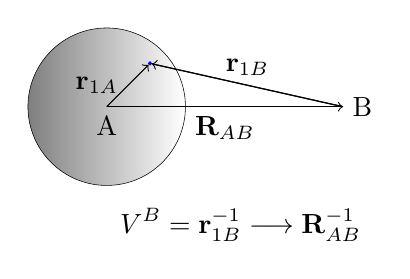
\begin{tikzpicture}
			%	\filldraw (elec)circle(.1);
			\coordinate(B) at(3,0);
			\shade[draw, very thin, left color=gray, right color=white] (0,0)circle (1);
			\node[inner sep=.07,draw=blue,circle,fill=blue] (elec)at(.55,.55){};
			\filldraw[->](0,0)node[below]{A}--node[above,left]{$\mathbf{r}_{1A}$} (elec);
			\draw[->] (0,0)--node[below]{$\mathbf{R}_{AB}$}(B)node[right]{B};
			\draw(B)--node[above]{$\mathbf{r}_{1B}$}(elec);
			\draw[->] (B)--(elec);
			\draw(1.7,-1.5)node{$\displaystyle\braket{V^B}=\braket{\mathbf{r}_{1B}^{-1}}\longrightarrow \mathbf{R}_{AB}^{-1}$};
		\end{tikzpicture}
	\end{minipage}
	\begin{minipage}{.5\textwidth}
		\caption{邻近核对电子的吸引.}
		\label{f3.4}
	\end{minipage}
\end{figure}
\noindent 这就是单个电子在核势场中的\ha 矩阵, 即$\mathrm{H}_2^+$的\ha 矩阵. 
解矩阵本征值方程
\begin{align}
	\label{3.234}
	\mathbf{H}^\mathrm{core}\mathbf{C=SC}\bm{\epsilon}
\end{align}
就能得到$\mathrm{H}_2^+$的分子轨道核轨道能量. 
对于其他分子例如$\mathrm{H}_2\mathrm{O}$, 
如上方程会得到$\mathrm{H}_2\mathrm{O}^{9+}$的分子轨道核轨道能量, 
我们不关心这样的情况.


在极小基模型中的$2^4=16$个双电子积分$(\mu\nu|\lambda\sigma)$中, 
只有四个不一样的值
\begin{equation}
	\begin{split}
		(\phi_1\phi_1|\phi_1\phi_1) & = (\phi_2\phi_2|\phi_2\phi_2) = 0.7746\au\\
		(\phi_1\phi_1|\phi_2\phi_2) & =0.5679\au\\
		(\phi_2\phi_1|\phi_1\phi_1) & =(\phi_2\phi_2|\phi_2\phi_1)\au\\
		(\phi_2\phi_1|\phi_2\phi_1) & =0.2970\au
	\end{split}
\end{equation}
以上式经过指标的简单置换就得到其他积分, 
如$(\mu\nu|\lambda\sigma)=(\mu\nu|\sigma\lambda)=(\lambda\sigma|\mu\nu)$. 
单中心积分如$(\phi_1\phi_1|\phi_1\phi_1),(\phi_2\phi_2|\phi_2\phi_2)$就是同在$1s$轨道上的两电子间的平均排斥. 
双电子积分$(\phi_1\phi_1|\phi_2\phi_2)$是中心1上的轨道核中心2上的轨道间的电子排斥. 
其值为$0.5679\au$(在$R=1.4\au$下), 
当核间距$R$增大时它会趋于$1/R$. 
其他两个积分没有经典诠释. 
在大键长下这两个积分趋于零因为$S_{12}$趋于零. 
得到所有的基本积分后, 
下一步就能求解Roothaan方程:按之前所述的手续, 
就是初猜密度矩阵, 
构建Fock矩阵, 
将Fock矩阵变换到正交轨道基下, 
对角化变换后的Fock矩阵等等. 
不过此处的\phrase{极小基 $\hd$}模型过于简单, 
因此Roothaan方程的解可以简单地通过对称性确定. 
正则分子轨道构成分子点群的一个表示. 
也就是说, 
对于同核双原子分子, 
轨道可以标为$\sigma_g$、$\sigma_\mu$、$\pi_g$、$\pi_\mu$等等. 
在极小基下只有两个分子轨道. 
能量低的那个就是占据分子轨道, 
是具有$\sigma_g$对称的成键轨道
\begin{align}
	\psi_1 = [2(1+S_{12})]^{-1/2}(\phi_1+\phi_2)
\end{align}
虚分子轨道就是对应的反键轨道, 
对称性为$\sigma_\mu$:
\begin{align}
	\psi_1 = [2(1-S_{12})]^{-1/2}(\phi_1-\phi_2)
\end{align}
该问题的最终系数矩阵成为
\begin{align}
	\mathbf{C}=
	\begin{pmatrix}
		[2(1+S_{12})]^{-1/2} & [2(1-S_{12})]^{-1/2}\\
		[2(1+S_{12})]^{-1/2} & -[2(1-S_{12})]^{-1/2}\\
	\end{pmatrix}
\end{align}
最终密度矩阵为
\begin{align}
	\mathbf{P}=
	\begin{pmatrix}
		(1+S_{12})^{-1} & (1+S_{12})^{-1} \\
		(1+S_{12})^{-1} & (1+S_{12})^{-1} \\
	\end{pmatrix}
	=(1+S_{12})^{-1} 
	\begin{pmatrix}
		1&1\\1&1
	\end{pmatrix}
\end{align}
若SCF手续中初猜的密度矩阵与上式不同, 
那么就要进行迭代, 
该手续会收敛到这个由对称性所决定的解上.

\exercise{对$\psi_1,\psi_2$进行归一化, 由此导出$\psi_1,\psi_2$的基函数展开中的系数$[2(1+S_{12})]^{-1/2}$及$[2(1-S_{12})]^{-1/2}$.
	\Next
	\phrase{极小基 $\hd^+$}的系数同样可由对称性决定, 办法与\phrase{极小基 $\hd$}一样. 
	用以上所得系数求解\autoref{3.234}, 得到\phrase{极小基 $\hd^+$}在$R=1.4\au$的轨道能量, 验证它们是
	\begin{align*}
		\epsilon_1 = (H_{11}^\mathrm{core} + H_{12}^\mathrm{core})(1+S_{12}) = -1.2528\,\mathrm{a.u}\\
		\epsilon_2 = (H_{11}^\mathrm{core} - H_{12}^\mathrm{core})(1--S_{12}) = -0.4756\,\mathrm{a.u}.
	\end{align*}
	\Next
	用密度矩阵的一般定义(3.
	145)导出(3.
	239). 
	并指出$\hd^+$对应的密度矩阵是什么?
	\Next
	用Fock矩阵的一般定义(3.
	154)证明它在\phrase{极小基 $\hd$}下矩阵元的收敛值为
	\begin{align*}
		F_{11} = F_{22} = &H^\mathrm{core}_{11} + (1+S_{12})^{-1}[\frac{1}{2}(\phi_1\phi_1|\phi_1\phi_1)+(\phi_1\phi_1|\phi_2\phi_2)\\
		&+ (\phi_1\phi_1|\phi_1\phi_2)-\frac{1}{2}(\phi_1\phi_2|\phi_1\phi_2) ] = -0.3655\au\\
		F_{12} = F_{21} = &H^\mathrm{core}_{12} + (1+S_{12})^{-1}[-\frac{1}{2}(\phi_1\phi_1|\phi_1\phi_1)+(\phi_1\phi_1|\phi_1\phi_2)\\
		&+ \frac{3}{2}(\phi_1\phi_2|\phi_1\phi_2) ] = -0.5939\au
	\end{align*}
	\Next
	用练习(3.
	23)的结果证明\phrase{极小基 $\hd$}的轨道能量, 
	也就是Roothaan方程$\mathbf{FC=SC}\bm{\epsilon}$的解, 
	是
	\begin{align*}
		\epsilon_1 = (F_{11}+F_{12})/(1+S_{12}) = -0.5782\au\\
		\epsilon_2 = (F_{11}-F_{12})/(1+S_{12}) = +0.6703\au
	\end{align*}
	\Next
	用总电子能量的一般\autoref{3.184}证明\phrase{极小基 $\hd$}的电子能量为
	\begin{align*}
		E_0 = (F_{11}+H^\mathrm{core}_{11}+F_{12}+H^\mathrm{core}_{12})/(1+S_{12}) = -1.8310\au
	\end{align*}
	包含核排斥的总能为
	\begin{align*}
		E_\mathrm{tot} = -1.1167\au
	\end{align*}
}
上面三个练习中\phrase{极小基 $\hd$}的结果全部是由基组$\{\phi_\mu\}$的积分和矩阵表示的, 
而不是用(\hft)方程的解$\{\psi_i\}$来表示, 
这就是实际计算中所用的方式, 
分子轨道$\{\psi_i\}$直到计算完成后才能得到. 
为了讨论SCF的结果, 
而且后面处理相关效应时也会用到这里的SCF结果, 
我们将上面以${\phi_{\mu}}$表示的基本积分换用${\psi_i}$表示. 
我们知道两组函数间的关系:
\begin{align}
	\psi_i = \sum_{\mu=1}^{K}C_{\mu i}\phi_\mu
\end{align}
那么变换按下式进行
\begin{align}
	h_{ij} & = (\psi_i|h|\psi_j) = \sum_{\mu}\sum_{\nu}C_{\mu i}^*C_{\nu j}H_{\mu\nu}^\mathrm{core}\\
	(\psi_i\psi_j|\psi_k\psi_l) & = \sum_\mu\sum_\nu\sum_\lambda\sum_\sigma C_{\mu i}^*C_{\nu j}C_{\lambda k}^*C_{\sigma l}(\mu\nu|\lambda\sigma)
\end{align}
(3.241)中的双指标变换相对容易, 所要做的无非是$K\times K$矩阵的乘法. 
但是双电子积分的四指标变换非常耗时. 做这种变换时, 即使是优化的算法也要用$O(K^5)$次乘法. 其难度比整个SCF手续中的任意一步都多至少$K$阶. 
若不需要变换双电子积分, 那么就无需以上计算. 另一方面. 多数超过\hft 的办法及本书所考虑的所有方法, 都需要分子轨道的积分. 
在\phrase{极小基 $\hd$}模型中, 这种变换当然不难. 
核心哈密顿矩阵经变换后的非零矩阵元和双电子积分矩阵如下
\begin{align*}
	h_{11} & =(\psi_1|h|\psi_1)=-1.2528\au          &  & h_{22}=(\psi_2|h|\psi_2)=-0.4756\au          \\
	J_{11} & =(\psi_1\psi_1|\psi_1\psi_1)=0.6746\au &  & J_{22}=(\psi_2\psi_2|\psi_2\psi_2)=0.6975\au \\
	J_{12} & =(\psi_1\psi_1|\psi_2\psi_2)=0.6636\au &  & K_{12}=(\psi_1\psi_2|\psi_2\psi_1)=0.1813\au
\end{align*}
如前面所述, 
$h_{11}$是$\psi_1$上一个电子的动能加上核吸引势能, 
$h_{22}$是$\psi_2$上电子的, 
$J_{11}$是$\psi_1$是哪个两个电子间的库伦排斥, 
$J_{22}$是$\psi_2$上的两电子间的库伦排斥, 
$J_{12}$是$\psi_1,\psi_2$上电子间的, 
$-K_{12}$是$\psi_1$上一个电子与$\psi_2$上同自旋电子间的交换作用.


变换后的Fock矩阵, 
$f_{ij}=(\psi_i|f|\psi_j)$根据定义是对角阵, 
对角元等于轨道能量. 
闭壳层轨道能量在练习3.9中推导过, 
为
\begin{align}
	\epsilon_i = h_{ii} + \sum_b2J_{ib} -K_{ib}
\end{align}
在此处的极小基模型中, 
它们是
\begin{align}
	\epsilon_1 & = h_{11} + J_{11} = -0.5782\au\\
	\epsilon_2 & = h_{22} + 2J_{12} - K_{12} = +0.6703\au
\end{align}
注意到$\epsilon_2\neq h_{22}+J_{22}$, 
因为它是一个虚轨道, 
描述的是$(N+1)$-电子体系中电子的能量, 
这已经在Koopmans定理那里提过了. 
附录D中列出了不同键长下轨道能量以及双电子积分$J_{11}$等等量的值. 
利用这些数值可以(本章及之后)研究一批多电子量作为键长的函数的行为.


基态的总电子能量为
\begin{align}
	E_0 = 2h_{11} + J_{11} = -1.8310\au
\end{align}
包含核排斥的总能为
\begin{align}
	E_\mathrm{tot} = E_0 + 1/R = -1.1167\au
\end{align}
由于在这个基下氢原子的能量为$-0.4666\au$. 
那么预测的$\hd$解离能就是$2(-0.4666)+1.1167=0.1835\au\equiv 4.99\,\mathrm{eV}$. 
作为比较, 
解离能实验值为$4.75\,\mathrm{eV}$, 
符合得很好, 
虽然计算所得的$\hd$能量比精确值高得多, 
但是计算所得氢原子的能量也不精确, 
如此有一个抵消.


上面得到的解离能与实验符合得很好, 但要完整地回答解离问题, 还需要研究整个势能面. 
在不同核间距下重复以上计算就得到\autoref{f3.5}中所绘的势能面, 
图中也绘出了由Kolos和Wolniewicz\endnote{
	W. Kolos and Wolniewics, Improved theoretical ground-state energy of the hydrogen molecule, \textit{J. Chem. Phys.} \textbf{49:} 404 (1968).
}得到的十分精确的结果. 
极小基限制性\hft 计算没有给出$R$趋于无穷时的极限. 
初想这个结果好像比较奇怪. 其实这种完全错误的行为并非$\hd$系统独有.
\begin{figure}[H]\centering
	\begin{tikzpicture}
		\begin{axis}[
			axis y line*=middle,
			axis x line*=middle, 
			tick label style={
				/pgf/number format/fixed,
				/pgf/number format/fixed zerofill,
				/pgf/number format/precision=1
			},
			xtick={1.0,2,3,4,5,6},
			xticklabel style={anchor=south},
			xticklabel shift={-3pt},
			ytick={-.2,-.1,0,.1,.2,.3,.4,.5,.6},
			ymin=-.2,
			ymax=0.6,
			xmin=0,
			xmax=6,
			height=.8\textwidth,
			width=.7\textwidth,
			every axis x label/.style={at={(axis cs:6.85,.034)}}, xlabel={$R$(a.u.)},
			every axis y label/.style={rotate=90,at={(axis description cs:-.15,.5)}},
			ylabel={$E(\hd)-2E(\mathrm{H})\,(\au)$},
			]
			\addplot [domain=.26:6, thick, mark=none, blue] table{./Pictures/h2.dat};
			\addplot [domain=.26:6, thick,dashed, mark=none, blue] table{./Pictures/wolniewicz.dat};
			\draw[<-] (axis cs:2.7,-.08578740)--(axis cs:3.2,-.08578740)node[right]{精确};
			\draw     (axis cs:3.8,-.12)node{(Kolos-Wolniewicz)};
			\draw[<-] (axis cs:4.05,.17)--(axis cs:4.4,.17)node[right]{STO-3G};
			\draw (axis cs:2.4,.38)circle(7pt);
			\draw (axis cs:3.6,.38)circle(7pt);
			\draw[<->](axis cs:2.4,.38)--node[above]{$R$}(axis cs:3.6,.38); 
		\end{axis}
	\end{tikzpicture}
	\caption{$\hd$的STO-3G限制性\hft 势能曲线与Kolos和Wolniewicz的精确结果对比.}
	\label{f3.5}
\end{figure}
若将键拉长, 
导致正确的解离产物必须用开壳层波函数来描述的话, 
这里的限制性闭壳层计算给出的极限肯定是错误的. 
对于$\hd$, 
解离产物是两个定域的氢原子, 
也即, 
一个电子局域在一个质子附近. 
另外一个电子局域在另一个相隔很远的质子附近. 
但是在限制性计算中, 
两个电子被强制放在一个空间分子轨道$\psi_1$上. 
这个分子轨道由对称性决定, 
形式为(3.236). 
因此, 
无论键长如何, 
两个电子都确实被同一个空间波函数描述, 
在三维空间中的概率分布也相同. 
这种描述对两个隔开的氢原子是不合适的. 
限制性闭壳层\hft 计算中,电子被强制成对放在分子轨道上, 
因此无法正确描述解离, 
除非解离产物都是闭壳层的.


我们可用练习3.25和练习3.27中的结果分析地研究解离行为. 
当$R\to\infty$时, 
\autoref{f3.4}中的双中心核吸引趋于零, 
$H_{11}^\mathrm{core}\to T_{11}+V_{11}^1$, 
这就是当前基下氢原子的能量($-0.4666$). 
除单中心电子电子排斥积分$(\phi_1\phi_1|\phi_1\phi_1)$外, 
其他积分在$R\to \infty$时都趋于零. 
因此就有
\begin{align*}
	\lim_{R\to\infty} E_\mathrm{tot}(R) & = \lim_{R\to\infty} 2H_{11}^\mathrm{core} + \frac{1}{2}(\phi_1\phi_1|\phi_1\phi_1) \\
	& = 2E(H) + \frac{1}{2}(\phi_1\phi_1|\phi_1\phi_1)                                   \\
	& = -0.9332 + 0.3873                                                                 \\
	& = -0.5459\au
\end{align*}
这个极限值不等于当前基下氢原子能量的两倍($2E(\mathrm{H})$), 
而是多出一个不正确的项$\frac{1}{2}(\phi_1\phi_1|\phi_1\phi_1)$. 
这个额外项出现的原因是两个电子占据了同一空间轨道, 
在无穷远距离下它们仍有排斥. 
或者说, 此时解离产物不仅是$2\mathrm{H}\cdot$, 
还错误地包含了$\mathrm{H}^+,\mathrm{H}^-$. 
$\mathrm{H}^-$的能量中含有电子-电子排斥积分$(\phi_1\phi_1|\phi_1\phi_1)$的贡献. 
另一种看这个问题的方式是, 
分子轨道波函数等价于离子项和共价项等权重的价键波函数. 
由于这里的波函数由对称性确定, 
那么离子项即使在解离时也仍存在. 
之后讨论非限制性\hft 计算时会继续探讨解离问题.


当解离为开壳层产物时, 
限制性闭壳层\hft 计算表现很差, 
但这无损于其在平衡点附近的用处. 
计算所得的平衡构型就是$E_\mathrm{tot}$关于的核坐标最小时的构型. 
\autoref{t3.2}列出了实验核间距$1.4\au$领域内的总能量值. 
计算得到最小能量是在$1.346\au$处. 
误差为$4\%$, 
我们可以预估, 
计算其他分子时所得的平衡构型误差也在类似的量级上. 

\begin{table}[H]
	\centering
	\caption{极小基STO-3G下$H_2$的能量与键长的关系}
	\begin{tabular}{cc}
		\hline
		$R \mathrm{(a.u)}$ & $E_\mathrm{tot}\mathrm{(a.u.)}$\\\hline
		1.32      & -1.11731\\
		1.34     & -1.11750\\
		1.36     & -1.11745\\
		1.38     & -1.11719\\
		1.40     & -1.11672\\\hline
		\multicolumn{2}{c}{$R_\mathrm{eq}$=1.346 a.u.}
	\end{tabular}
	\label{t3.2}
\end{table}
\begin{table}[H]
	\centering
	\caption{R=1.4 a.u.时对极小基STO-3G下$H_2$的Slater指数的优化}
	\begin{tabular}{cc}
		\hline
		$\zeta$ & $E_\mathrm{tot} \mathrm{(a.u.)}$\\\hline
		1.0      & -1.08164\\
		1.1     & -1.11089\\
		1.2     & -1.11912\\
		1.3     & -1.10714\\\hline
		\multicolumn{2}{c}{$\zeta_\mathrm{optimum}$=1.19}
	\end{tabular}
	\label{t3.3}
\end{table}
讨论焦点离开\phrase{极小基 $\hd$}前(至少是暂时离开), 
我们要用这个模型来解释指数优化(exponent optimization). 
之前所用的标准指数为$\zeta=1.24$. 
轨道指数是波函数中的非线性参数. 
用变分原理可知, 
这个形式下的最优函数就是关于波函数中所有参数能最小的那个. 
但轨道指数是非线性参数, 
没有很容易的计算方式来确定其最优值. 
一般不会费时对不同的轨道指数进行大量计算来找到最优值, 
而是预先选取合理的``标准''值, 
就如氢的$1s$轨道下STO-3G的值设为$1.24$. 
若要求更好的精确度, 
可以增加基组的尺寸. 
然而有时也需要或想要对指数进行优化, 
如果没有其他合适理由来确定``合理''值到底是多少. 
\autoref{t3.3}列出了不同$1s$ Slater轨道指数$\zeta$下的\phrase{极小基 $\hd$}($R=1.4$)总能量. 
$R=1.4\au$时最优指数为$1.14$. 
最优值会随键长改变, 
而且对其他分子中的氢原子其值也会不同. 
但是我们可以发现, 
一大批分子中这个最优值都大于$1.0$(单个氢原子的精确值), 
标准的STO-3G基组中我们选取$1.24$作为一批小分子中最优值的代表. 
$\hd$中最优值为$1.19$证明氢分子某种程度上比两个氢原子之和更``小”. 
这在化学成键中很普遍——成键电子与两个核间的吸引(单个原子情况下电子云只与一个核有吸引)致使电子云收缩. 

\subsection{STO-3G下的HeH$^+$: SCF计算}
双电子分子$\hd$和$\heh$分别是同核/异核双原子分子的原型. 
我们刚才已经完成了\phrase{极小基STO-3G $\hd$}的计算, 
现在对\phrase{极小基 $\heh$}也做同样的计算. 
这些描述双电子体系的极小基模型唯一的限制就是基组. 
用大基组就可以得到更精确的结果, 
但此处小基组就足以说明我们的问题了. 
扩展到大基组的非常直接的. 


最然极小基很小, 
但能够得到在这些基函数所张的单电子空间内的精确结果. 
特别的, 
使用极小基可以研究任意多中方法并将其结果与``真实''结果作比较. 
后面各章我们会用与此处相同的\phrase{极小基STO $\hd,\heh$}模型来说明组态相互计算、微扰论计算等等方法. 
那里所得的结果会与相同基组下的精确结果研究本章的\hft 计算做比较.


\phrase{极小基 $\hd$}的一个缺点是它只有两个基函数, 
分子轨道有对称性上的缺点, 没办法展示出SCF手续的迭代特性. 
而$\heh$是异核分子, 它的对称性少于$\hd$, 而且这个极小基模型的分子轨道无法由对称性决定. 
由此, 对$\heh$做限制性\hft 计算就能完全展示求解Roothaan方程所涉及的原理. 

带一个电荷的氦氢分子离子在质谱研究中已经被熟知很多年了.
在天体物理问题中, 人们也关心该离子, 
因为它是质子散射$\mathrm{He}$中$\mathrm{HT}$经$\beta$衰变的产物,
此外还有与其简单性相关的其他各种原因. 
但是在实验上好像很少有对该离子不同电子态结构的研究.
Wolniewicz做过非常精确的计算\endnote{
L. Wolniewics, Variational treatment of the $\heh$ ion and the $\beta$-{decay} in HT, \textit{J. Chem. Phys.} \textbf{43:} 1078 (1965).
}; 计算表明它的基态的平衡键长为$1.4632\au$, 电子键能为$0.0749\au(2.309\,\mathrm{eV})$. 
在基态下解离会生成氦原子和质子:
\begin{align}
	\heh(X^1\Sigma) \to \mathrm{He}(^1S) + \mathrm{H}^+
\end{align}
而不是$\mathrm{He}^+ + \mathrm{H}$. 
因为$\mathrm{He}$的电离能(24.6eV)比质子的电子亲和能(13.6eV)大. 
或者说, 
$\mathrm{He}^+$的电子亲和能比$\mathrm{H}^+$的电子亲和能大. 
所涉不同物种的精确能量列在\autoref{t3.4}中. 
由于解离产物是闭壳层的, 
我们可以预期, 
限制性\hft 计算在大键长下的行为应当正确, 
不会发生$\hd$中那种情况. 

\begin{table}[H]
	\centering
	\caption{H和He不同物种的精确能量}
	\begin{tabular}{cc}
		\hline
		物种 & 能量(a.u.)\\\hline
		H$^+$      & 0.0\\
		H     & -0.5\\
		He$^+$     & -2.0\\
		He     & -2.90372\\
		HeH$^+$(R = 1.4632 a.u.)&-2.97867\\\hline
	\end{tabular}
	\label{t3.4}
\end{table}
要进行SCF计算, 首先要选定核构型. 
我们记氦核为核1, 其位置矢量为$\mathbf{R}_1$, 
氢核为核2, 其位置矢量为$\mathbf{R}_2$, 
那么$|\mathbf{R}_1-\mathbf{R}_2|=R_{12}$就是核间距. 
我们使用精确核间距$R=1.4632\au$. 
然后要确定基组, 此处使用极小基STO-3G. 
每个核上有一个$1s$轨道:
\begin{align}
	\phi_1 \simeq (\zeta_1^3/\pi)^{1/2} e^{-\zeta_1|\mathbf{r-R}_1|}\\
	\phi_2 \simeq (\zeta_2^3/\pi)^{1/2} e^{-\zeta_2|\mathbf{r-R}_1|}
\end{align}
基函数由三个原初高斯型收缩而成, 
收缩系数(3.221), 
收缩指数是(3.221)中的按比例乘以$\zeta_1$或$\zeta_2$的平方. 
现在只要确定$\mathrm{He}$的Slater指数$\zeta_1$和$\mathrm{H}$的Slater指数$\zeta_2$. 
分子环境中的$\mathrm{H}$有标准STO-3G指数$\zeta_2=1.24$, 
这就是在\phrase{极小基 $\hd$}中使用的值. 
而$\mathrm{He}$没有这样的标准STO-3G指数. 
分子计算中选择指数时场会用同一基组计算单个原子的能量, 
指数选为对应能量最小的那个. 
这种指数有时叫作``最优原子''指数. 
对氢来说最优原子指数为1.0. 
若对$\mathrm{He}$做限制性\hft 计算, 
使用只含一个Slater轨道$(\zeta^3/\pi)^{1/2}e^{-\zeta r}$的基组, 
可以得到最优原子指数为$27/16=1.6875$. 
这个值(27/16)的推导是变分原理的经典教科书例子\endnote{
I. N. Levine, Quantum Chemistry, Allyn and Bacon, Boston, 1974, p. 190 .
}.
由于$\heh$有一个净的正电荷, 
我们预想电子云相比在独立原子$\mathrm{He,H}$中会有明显收缩. 
为了说明问题我们会对$\mathrm{H}$用标准的STO-3G值$\zeta_2=1.24$, 
对$\mathrm{He}$用$\zeta_1=1.6875\times 1.24=2.095$, 
这个值和氢的值一样, 
都比最优原子值大$1.24$倍. 
如前所述, 
\autoref{f3.6}或(3.249)(3.250)中每个STO-3G函数都是三个原初高斯型之和.


计算的下一步, 
或者说多数\emph{从头算}的下一步就是计算所需的基函数积分. 
附录A中说明了$1s$高斯函数的积分如何计算并给出值涉及$1s$高斯函数的直接积分公式. 
附录B给出了一个FORTRAN程序以及$\heh$情形的输出, 
这个程序展示了求解Roothaan方程的完整步骤, 
它可在极小基下用高斯函数对所有双电子的双原子分子进行计算. 

\begin{figure}[H]\centering
	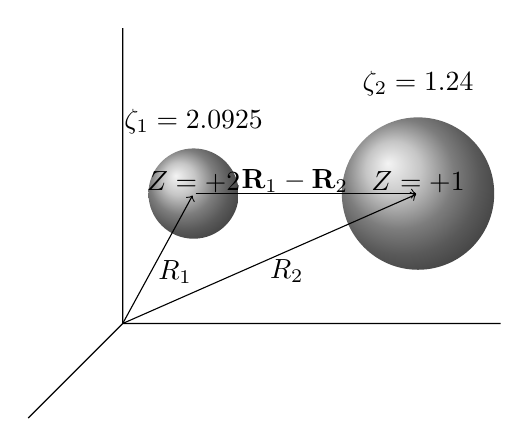
\begin{tikzpicture}[scale=1.5,inner sep=.1]
		\node (R1) at (.6,1.1){};
		\node (R2) at (2.5,1.1){};
		\shade[ball color=black!30] (R1)circle(.477897252*0.8);
		\shade[ball color=black!30] (R2)circle(.806451613*0.8);
		%orbital exponent \xi for Z=+2 is 2.0925 and 1.24 for Z=+1. The maximum of radial relectron density is 1/\xi, namely 0.477897252 for Z=+2 and 0.806451613 for Z=+1.
		\draw(0,2.5)--(0,0)--(3.2,0) (0,0)--(-.8,-.8);
		\draw[->] (0,0)--node[below right,pos=.5]{$R_1$}(R1);
		\draw[->] (0,0)--node[below right]{$R_2$}(R2);
		\draw[->] (R1)node[above]{$Z=+2$}--node[above,pos=.45]{$\mathbf{R}_1-\mathbf{R}_2$}(R2)node[above]{$Z=+1$};
		\draw (R1)+(0,0.5)node[above]{$\zeta_1=2.0925$} (R2)+(0,0.82)node[above]{$\zeta_2=1.24$};
	\end{tikzpicture}
	\caption{\phrase{极小基STO-3G $\heh$}计算时所用的坐标系和基函数.}
	\label{f3.6}
\end{figure}此处仅给出结果, 必要时读者可以参考附录B中的程序输出. 由附录A可知, 两个基函数的重叠随核间距指数减少. 核间距为$R=1.4632\au$时, 重叠的值为$S_{12}=S_{21}=0.4508$. 这个重叠要小于$\hd$中的, 因为$\mathrm{He}$的轨道比$\mathrm{H}$的相应轨道更小、更定域. 由此, 重叠矩阵为
\begin{align}
	\mathbf{S} = \begin{pmatrix}
		1.0 & 0.4508\\0.4508&1.0
	\end{pmatrix}
\end{align}
动能矩阵为
\begin{align}
	\mathbf{T} = \begin{pmatrix}
		2.1643&0.1670\\0.1670&0.7600
	\end{pmatrix}
\end{align}
$T_{22}$的值与$\hd$中的值一样, 因为所用指数相同. $T_{11}$的值代表的是$\mathrm{He} 1s$轨道中一个电子的动能, 比$\mathrm{H}$的要大, 这反映了$\mathrm{He}$轨道的大指数, 大指数反之又说明$\mathrm{He}$的核电荷比$\mathrm{H}$大. 电子距核的平均距离越小动能就越大.

核1(氦核)的吸引势能矩阵为
\begin{align}
	\mathbf{V}^1 = 
	\begin{pmatrix}
		-4.1398&-1.1029\\-1.1029&-1.2652
	\end{pmatrix}
\end{align}
$\phi_1$所在核对$\phi_1$上电子的单中心吸引(-4.1398)很自然比另外一个距离较远的轨道$\phi_2$上电子所受的(-1.2652)更强. 后者这个双中心积分在大核间距下趋近$-2/R$. 非对角元,即氦核对由乘积分布$\phi_1(1)\phi_2(1)$所描述的电子的吸引完全是导致成键的量子力学项.

核2(氢核)的核吸引矩阵与上面类似, 
但数量上更小, 
因为质子的核电荷比氦核少:
\begin{align}
	\mathbf{V}^2 = 
	\begin{pmatrix}
		-0.6772&-0.4113\\-0.4116&1.2266
	\end{pmatrix}
\end{align}
$V_{22}^2$与$\hd$中的相同. 函数$\phi_1$的指数更大, 因此相对更定域在$\mathrm{He}$附近, $V_{11}^2$很接近它的渐近值$-1/R=-0.6834$.

得到动能及核吸引积分后就能构建芯-\ha 矩阵:
\begin{align}
	\mathbf{H}^\mathrm{core} = \mathbf{T+V}^1 + \mathbf{V}^2=
	\begin{pmatrix}
		-2.6527&-1.3472\\-1.3472&-1.7318
	\end{pmatrix}
\end{align}
正如我们之前所说, 
这就是单个电子在核势场中的正确\ha 矩阵. 
芯-\ha 的类-Roothaan方程为
\begin{align}
	\mathbf{H}^\mathrm{core}\mathbf{C=SC}\bm{\epsilon}
\end{align}
由该式可得到单个电子在$\mathrm{HeH}^{++}$势场中的分子轨道及轨道能量(在当前例子下就是总电子能量). 
而电子-电子排斥效应对分子轨道和能量的影响(在单行列式框架下)就体现在矩阵$\mathbf{G}$上;
$\mathbf{G}$加$\mathbf{H}^\mathrm{core}$就得到$\mathbf{F}$.


最后剩余的积分就是双电子排斥积分. 
在$2^4=16$个可能的积分$(\mu\nu|\lambda\sigma)$中只有六个相异值:
\begin{align*}
	(\phi_1\phi_1|\phi_1\phi_1)&=1.3072\au& (\phi_2\phi_2|\phi_1\phi_1)&=0.6057\au\\
	(\phi_2\phi_1|\phi_1\phi_1)&=0.4373\au& (\phi_2\phi_2|\phi_2\phi_1)&=0.3118\au\\
	(\phi_2\phi_1|\phi_2\phi_1)&=0.1773\au& (\phi_2\phi_2|\phi_2\phi_2)&=0.7746\au\\
\end{align*}
单中心积分$(\phi_1\phi_1|\phi_1\phi_1)$和$(\phi_2\phi_2|\phi_2\phi_2)$就是$\phi_1$(或$\phi_2$)内一个电子与同轨道内另外一个电子之间的排斥. 
较小的函数$\phi_1$内两个电子的平均距离比较大且更弥散的函数$\phi_2$中的平均距离更大, 
因此$(\phi_1\phi_1|\phi_1\phi_1)$大于$(\phi_2\phi_2|\phi_2\phi_2)$. 
双中心积分$(\phi_2\phi_2|\phi_1\phi_1)$是$\phi_1$内电子与$\phi_2$内电子间的排斥. 
当核间距增大时它的渐近值为$1/R$. 
其他三个积分没有简单的经典诠释.


到此我们就有了$\heh$ SCF计算所需的全部积分. 
但在开始迭代前, 
需导出使基函数正交化所需的变换矩阵:
\begin{align}
	\phi_\mu'=\sum_\nu X_{\mu\nu}\phi_\nu
\end{align}
可导出正交化函数集合$\phi_\mu'$的矩阵$\mathbf{X}$有很多. 
第一章讨论的Schmidt方案中, 
使用了如下矩阵
\begin{align}
	\mathbf{X}_\mathrm{Schmidt} = 
	\begin{pmatrix}
		1 & -S_{12}/(1-S_{12}^2)^{1/2} \\
		0 & 1/(1-S_{12}^2)^{1/2}
	\end{pmatrix}=
	\begin{pmatrix}
		1.0 & -0.5050 \\
		0.0 & 1.1203
	\end{pmatrix}
\end{align}
\exercise{
	证明以上变换确实可将基函数正交化.
	
}
其他两种方案之前也已提过, 
这两种方案需要对角化重叠矩阵. 
对角化$2\times2$矩阵可用1.1.6节中的方法. 
对于此处的重叠矩阵, 
本征值就是$s_1=1+S_{12}=1.4508,s_2=1-S_{12}=0.5492$. 
进行对角化的酉矩阵为
\begin{align}
	\mathbf{U}=
	\begin{pmatrix}
		[2]^{-1/2}&[2]^{-1/2}\\
		[2]^{-1/2}&-[2]^{-1/2}
	\end{pmatrix}
\end{align}
要导出对称化/正则正交变换矩阵就需要如下矩阵
\begin{align}
	\mathbf{s}^{-1/2}=
	\begin{pmatrix}
		s_1^{-1/2}&0\\0&s_2^{-1/2}
	\end{pmatrix}=
	\begin{pmatrix}
		0.8302&0.0\\0.0&1.3493
	\end{pmatrix}
\end{align}
对称正交化中我们使用如下变换矩阵
\begin{align}
	\mathbf{X}_\mathrm{symmetric} = \mathbf{S}^{-1/2}=\mathbf{Us}^{-1/2}\mathbf{U^\dagger}=
	\begin{pmatrix}
		1.0898&-0.2596\\-0.2596&1.0898
	\end{pmatrix}
\end{align}
\begin{figure}[H]
	\begin{minipage}[b]{.6\textwidth}
		(a) Schmidt \qquad\begin{tikzpicture}[baseline=(current bounding box.center),scale=.7]
			\draw[->](0,0)--(3,0)node[below]{$\phi_1'$};
			\draw[->,dotted](0,0.1)--+(3,0)node[above]{$\phi_1$};
			\draw[->,dotted](0,0)--(45:3)node[below,right]{$\phi_2$};
			\draw[->](0,0)--(0,3)node[below,right]{$\phi_2'$};;
		\end{tikzpicture}
		
		(b) 对称 \qquad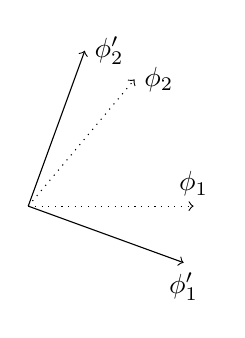
\begin{tikzpicture}[baseline=(current bounding box.center),scale=.7]
			\draw[->](0,0)--(-20:3)node[below]{$\phi_1'$};
			\draw[->,dotted](0,0)--(0:3)node[above]{$\phi_1$};
			\draw[->,dotted](0,0)--(50:3)node[below,right]{$\phi_2$};
			\draw[->](0,0)--(70:3)node[below,right]{$\phi_2'$};;
		\end{tikzpicture}
		
		(c) 正则 \qquad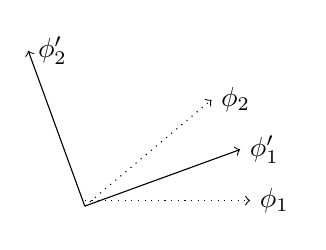
\begin{tikzpicture}[baseline=(current bounding box.center),scale=.7]
			\draw[->,dotted](0,0.1)--+(3,0)node[below,right]{$\phi_1$};
			\draw[->](0,0)--(20:3)node[below,right]{$\phi_1'$};
			\draw[->,dotted](0,0)--(40:3)node[below,right]{$\phi_2$};
			\draw[->](0,0)--(110:3)node[below,right]{$\phi_2'$};;
		\end{tikzpicture}
	\end{minipage}
	\begin{minipage}[t]{.4\textwidth}
		\caption{三种正交化方案:a) Schmidt; b) 对称; c)正则}
		\label{f3.7}
	\end{minipage}
\end{figure}
而正则正交化的变换矩阵为
\begin{align}
	\mathbf{X}_\mathrm{canonical}=\mathbf{Us}^{-1/2}=
	\begin{pmatrix}
		0.5871&0.9541\\0.5871&-0.9541
	\end{pmatrix}
\end{align}
这三种正交化方案的对比绘在图~\autoref{f3.7}中. 
原基函数之间的角度按$\cos\theta=S_{12}$定义. 
Schmidt正交化保持第一个基函数不动, 
令第二个与其正交. 
对称正交化所产生的两个新函数与原函数最为靠近. 
它的做法是将矢量之间的角度打开到$90^\circ$. 
正则正交化会产生一个平分原函数角度的新矢量, 
然后使第二个矢量与其正交. 
我们使用正则正交化, 
那么变换后的基函数为
\begin{align}
	\phi_1'=0.5871\phi_1 + 0.5871\phi_2\\
	\phi_2'=0.9541\phi_1 - 0.9541\phi_2
\end{align}

到此SCF迭代手续的准备工作已经完毕. 
我们现初猜一个密度矩阵. 
使用零矩阵比较方便. 
这等价于忽视所有电子-电子相互作用($\mathbf{G}$为零矩阵), 
并使芯-\ha 作为Fock矩阵的初猜:
\begin{align}
	\mathbf{F}\simeq=\mathbf{H}^\mathrm{core}=
	\begin{pmatrix}
		-2.6527&-1.3472\\-1.3472&-1.7318
	\end{pmatrix}
\end{align}
这种初猜最易想到, 
但是在复杂情况下表现会很差. 
下一步是将Fock矩阵变换到正则正交归一基组下:
\begin{align}
	\mathbf{F^\dagger=X^\dagger FX}=
	\begin{pmatrix}
		-2.4397&-0.5158\\-0.5158&-1.5387
	\end{pmatrix}
\end{align}
将此矩阵对角化, 
即求解
\begin{align}
	\mathbf{F'C'=C'}{\boldsymbol\epsilon}
\end{align}
得到系数酉矩阵
\begin{align}
	\mathbf{C'}=
	\begin{pmatrix}
		0.9104&0.4136\\0.4136&-0.9104
	\end{pmatrix}
\end{align}
以及两个本征值
\begin{align}
	\label{3.269}
	\bm{\epsilon}=
	\begin{pmatrix}
		-2.6741&0.0\\0.0&-1.3043
	\end{pmatrix}
\end{align}
原基函数下的系数矩阵为
\begin{align}
	\mathbf{C=XC'}=
	\begin{pmatrix}
		0.9291&-0.6256\\0.1398&1.1115
	\end{pmatrix}
	\label{3.270}
\end{align}
\autoref{3.270}\autoref{3.269}给出了$\mathrm{HeH}^{++}$的轨道和轨道能量, 
我们将其作为$\heh$的轨道和轨道能的初猜. 
注意最低分子轨道$\psi_1$主要由$\phi_1$组成(系数为0.9291), 
而仅混入了一点点$\phi_2$(系数0.1398). 
忽视电子-电子排斥后, 
电子倾向于聚集在$\mathrm{He}$附近因为它由更高的核电荷. 
而加入电子-电子排斥的效应后, 
随着一步步迭代, 
这种现象会被逐渐缓和掉, 
电子被``抹开”, 
以减小电子-电子排斥.


由(3.270)可以构建密度矩阵的第一个实际猜测
\begin{align}
	\mathbf{P}=
	\begin{pmatrix}
		1.7266&0.2599\\0.2599&0.0391
	\end{pmatrix}
\end{align}
$\mathbf{P}$的对角元说明大部分电子密度聚集在在$\mathrm{He}$附近而非$\mathbf{H}$附近. 
对此更恰当的理解可通过布居分析得到. 
(3.271)中的密度矩阵并非$\mathrm{HeH}^{++}$的(差一个因子2), 而是核势场中\emph{两个}无相互作用电子的密度矩阵.

由$\mathbf{P}$可构建对$\mathbf{G}$的猜测:
\begin{align}
	\mathbf{G}=\begin{pmatrix}
		1.2626&0.3740\\0.3740&0.9890
	\end{pmatrix}
\end{align}
以及新的Fock矩阵
\begin{align}
	\mathbf{F=H}^\mathrm{core}+\mathbf{G}=
	\begin{pmatrix}
		-1.3904&-0.9732 \\ -0.9732&-0.7429
	\end{pmatrix}
\end{align}
由于电子-电子相互作用是正值, 
即(3.272)$\mathbf{G}$中的元素为正数, 
所以这个新Fock矩阵中的元素比原来的芯-\ha 猜测(3.265)中的要正得多. 
有了新Fock矩阵就可以求解对应本征值问题, 
然后就能得到对$\mathbf{C,P}$的新猜测并重复以上整个过程直到自洽. 
附录B中有一个实现该过程的程序, 
还有当前例子——STO-3G $\heh$的程序输出. 
阅读输出文件时应配以接下来的描述.


\autoref{t3.5}中列出了不同迭代次数下密度矩阵的元素及对应电子能量. 
随着迭代进行, 
电荷在$\mathrm{H}$附近积累, 
在$\mathrm{He}$附近减少. 
要得到每次迭代后能量的变分值, 
需使用如下公式
\begin{align}
	E_0 = \frac{1}{2}\sum_\mu\sum_\nu P_{\nu\mu}(H_{\mu\nu}^\mathrm{core}+F_{\mu\nu})
\end{align}
而且其中的密度矩阵$\mathbf{P}$必须和构建$\mathbf{F}$时所用的一样. 
如此, 
一旦构建了新的$\mathbf{F}$, 
就能立马算出能量, 
而无需等到构建下一个新的$\mathbf{P}$. 

\autoref{t3.5}中能量从高至低单调收敛. 由于能量是个变分量, 所以能量的相对误差要小于波函数和密度矩阵的. 

最终的波函数和能量为
\begin{align}
	\mathbf{C} &= 
	\begin{pmatrix}
		0.8018&-0.7823\\0.3368&1.0684
	\end{pmatrix}\\
	\bm{\epsilon} &= 
	\begin{pmatrix}
		-1.5975&0.0\\0.0&-0.0617
	\end{pmatrix}
\end{align}
\begin{table}[H]
	\centering
	\caption{迭代过程中的密度矩阵和电子能量 (STO-3G $\heh$) }
	\begin{tabular}{ccccc}
		\hline
		迭代次数 & $P_{11}$ & $P_{12}$ & $P_{22}$ & $E_0(\mathrm{a.u.})$ \\ \hline
		1   &  1.7266  &  0.2599  &  0.0319  &      -4.141863       \\
		2   &  1.3342  &  0.5166  &  0.2000  &      -4.226492       \\
		3   &  1.2899  &  0.5384  &  0.2247  &      -4.227523       \\
		4   &  1.2864  &  0.5400  &  0.2267  &      -4.227529       \\
		5   &  1.2862  &  0.5402  &  0.2269  &      -4.227529       \\
		6   &  1.2861  &  0.5402  &  0.2269  &      -4.227529       \\ \hline
	\end{tabular}
	\label{t3.5}
\end{table}
最低的轨道——被占轨道$\psi_1$是成键轨道, 
由两个系数同号也能看出. 
它主要还是由$\mathrm{He}$波函数$\phi_1$组成. 
虚轨道$\psi_2$是反键轨道, 
它的两个系数符号相反. 
它含$\mathrm{H}$波函数$\phi_2$的成分更多, 
这也是它和$\psi_1$正交所要求的. 
利用Koopmans定理可以预测电离能和电子亲和能. 
预测到的电离能很大($1.5975\au=43.5 \,\mathrm{eV}$), 
这在阴离子物种中很自然. 
预测的电子亲和能则是正的($0.0617\au=1.7\,\mathrm{eV}$), 
这个预测值意味着$\heh$会结合一个电子. 
这不是说$\mathrm{HeH}$就是稳定分子, 
因为$\heh$的解离产物(即$\mathrm{He}+\mathrm{H}^+$)结合电子的能力更强($\mathrm{H}^+$的电子亲和能比$\heh$的电子亲和能加上解离能还要大).


用$\mathbf{PS}$的对角元可以做Mulliken布居分析. 
分析后知$\phi_1$上附带$1.53$个电子, 
$\phi_2$带$0.47$个电子.
$\mathrm{He}$的静电荷为$+0.47$, 
$\mathrm{H}$为$+0.53$. 
由这个预测结果就知道, 
总的形式电荷$+1$基本平分在两个原子上. 
借助带撇的相应矩阵(也就是正交归一基$\{\phi_\mu'\}$下的矩阵)可以进行L\"owdin 布居分析. 
氢轨道上附带的电子为
\begin{align}
	P'_{22} = (\mathbf{S}^{1/2}\mathbf{PS}^{1/2})_{22} = 2(\mathbf{S}^{1/2}\mathbf{C})^2_{12}=0.5273
\end{align}
这种办法计算出的电荷分离情况与之前类似, 
$\mathrm{He,H}$分别带有$+0.53,+0.47$的静电荷. 
注意数值与之前相反.


$\heh$的总能为电子能量加上核排斥势$2/R$, 数值为$-2.860662\au$. 
由我们的基本积分也可以确定$\mathrm{H,He^+,He}$的能量. 
在当前基下, $\mathrm{H}$原子的能量与$\hd$计算中国的能量相同: $T_{22}+V_{22}^2=-0.4666\au$. 
单电子原子$\mathrm{He}^+$在此基下的能量也类似$T_{11}+V_{11}^1=-1.9755\au$. 
$\mathrm{He}$原子在$\phi_1$上由两个电子, 它的总能除了包含动能、核吸引势外, 还有两个电子之间的排斥. 
因此$\mathrm{He}$的能量为$2(T_{11}+V_{11}^1)+(\phi_1\phi_1|\phi_1\phi_1)$. 
这些能量列在\autoref{t3.6}中以便与\autoref{t3.4}中的精确结果比较.

由\autoref{t3.6}中的结果可以算得如下过程的解离能:
\begin{align}
	\heh & \to \text{He} + \text{H}^+ \quad \Delta E = 0.2168\,\, \text{a.u.}\\
	\heh & \to \text{He}^+ + \text{H} \quad \Delta E = 0.4168\,\, \text{a.u.}
\end{align}
这正确预测了$\heh$的解离产物为闭壳层的$\text{He}+\text{H}^+$, 
而非开壳层的$\text{He}^++\text{H}$. 
解离能$0.2168\,\,\text{a.u.}=5.90\,\,\text{eV}$相比正确值$2.04\,\,\text{eV}$略大.
这这主要因为我们的$\text{He}$的指数是$2.0925$, 
虽然对于$\heh$比较合适, 
但对解离产物$\text{He}$的最优值$1.6875$而言,
仍大了不少. 
$\text{He}$的能量值相对于$\heh$的值而言, 
过于高了.

\begin{table}[h]
\begin{threeparttable}
	\begin{tabular}{lc}
		\hline
		\multicolumn{1}{c}{物种} & 能量(a.u.)  \\ \hline
		$\text{H}^+$             &    0.0    \\
		$\text{H}$               & -0.466582 \\
		$\text{He}^+$            & -1.975514 \\
		$\text{He}$              & -2.643876\tnote{a} \\
		$\heh$ ($R=1.4632$ a.u.) & -2.860662\tnote{b} \\ \hline
	\end{tabular}
	\begin{tablenotes}
		\item[a] C. L. Pekeris, \textit{Phys. Rev.} 115: 1217 (1959).
		\item[b] L. Wolniewicz, \textit{J. Cherm. Phys.} 43: 1807 (1965).
	\end{tablenotes}
\end{threeparttable}
	\centering\caption{$\text{H}$和$\text{He}$物种的能量(STO-3G基组: $\zeta_1=2.0925,\zeta_2=1.24$)}
	\label{t3.6}
\end{table}
\autoref{f3.8}中绘出了用标准指数计算得到的势能曲线, 同时也绘出了Wolniewicz所得的精确结果结果。 STO-3G计算所得的平衡键长是$1.3782\,\,\text{a.u.}$, 和精确结相当接近,但是势阱深度却被高估了。这里没有遇到$\hd$情形(\autoref{f3.5})下的问题: 解离行为正确,因为解离产物是闭壳层的。
\begin{figure}[htbp]\centering
	\newlength{\twoc}
	\settowidth{\twoc}{精确}
	\begin{tikzpicture}
		\begin{axis}[
			axis y line*=middle,
			axis x line*=middle, 
			tick label style={
				/pgf/number format/fixed,
				/pgf/number format/fixed zerofill,
				/pgf/number format/precision=1
			},
			xtick align=inside,
			xtick={0.5,1.0,1.5,2.0,2.5,3.0,3.5},
			ytick={-.3,-.2,-.1,0,0.0,.1,.2,.3,.4,.5,.6,.7,.8},
			xticklabel style={
				anchor=south,
				yshift=0.5ex
			},
			ymin=-.3,
			ymax=0.8,
			xmin=0.5,
			xmax=3.5,
			height=.8\textwidth,
			width=.7\textwidth,
			every axis x label/.style={at={(axis description cs:1.1,.2)}},
			xlabel={$R$(a.u.)},
			every axis y label/.style={rotate=90,at={(axis description cs:-.15,.5)}},
			ylabel={$E(\heh)-2E(\mathrm{He})\,(\au)$},
			]
			\addplot [domain=.26:6, thick, mark=none, blue] table[y expr=\thisrowno{1}+2.6438] {./Pictures/heh-tot-ener.txt};
			
			\addplot [domain=.035:6, thick,dashed, mark=none, blue] table[y expr = -(\thisrowno{3}-2.9037244)] {./Pictures/W-heh.dat};
			\draw[->] (axis cs:1.7,0.1)node[right,above]{\parbox{\twoc}{精确\\(Wolniewicz)}}--(axis cs:1.5,-.06578740);
			%	\draw     (1.8,0.1)node[right]{(Wolniewicz)};
			\draw[<-] (axis cs:2.1,-.17)--(axis cs:2.4,-.17)node[right]{STO-3G};
			\draw (axis cs:1.9,.38)circle(7pt)(axis cs:1.8,.38) (axis cs:2.5,.38)circle(7pt);
			\draw[<->] (axis cs:1.9,.38)--node[above]{$R$}(axis cs:2.5,.38);
			%	\draw[dashdotted] (1.7,0.387)--(2.5,0.387)node[right]{STO-2G};
			%	\draw[dotted] (1.7,0.444)--(2.5,0.444)node[right]{STO-1G};
			%	\draw (1.7,0.5)--(2.5,0.5)node[right]{SLATER};
		\end{axis}
	\end{tikzpicture}
	\caption{$\heh$的STO-3G($\zeta_\mathrm{He}=2.0925$, $\zeta_H=1.24$)限制性\hft 势能曲线与Kolos和Wolniewicz的精确结果对比.}
	\label{f3.8}
\end{figure}
亦如对$\hd$所做的那样,
我们能解析地考察解离行为。
当键拉伸时,
$\psi_1$中$\phi_1$的系数增加, 
$\phi_2$的系数减小,
电子越来越集中于$\text{He}$周围。
在极限情况下,
$\psi_1$就变为$\phi_1$。
虚轨道$\psi_2$与$\psi_1$正交,
因此变为纯的$\phi_2$, 
也即
\begin{equation}
	\mathbf{C}_{R\to\infty}=
	\begin{pmatrix}
		1.0&0.0\\0.0&1.0
	\end{pmatrix}
\end{equation} 
对应密度矩阵为
\begin{equation}
	\label{3.281}
	\mathbf{P}_{R\to\infty}=
	\begin{pmatrix}
		2.0&0.0\\0.0&0.0
	\end{pmatrix}
\end{equation}
令双电子积分为零,
就得到$R\to\infty$所对应的电子能量。
设为零后剩余的积分就是$T_{11}$, 
$T_{22}$, 
$V_{11}^1$, 
$V_{22}^2$, 
$(\phi_1\phi_1)$和$(\phi_2\phi_2|\phi_2\phi_2)$.

\exercise{利用电子能量表达\autoref{3.184},Fock矩阵表达\autoref{3.154}以及以及渐近矩阵\autoref{3.281}证明
	\begin{equation*}
		E_0(R\to\infty)=2T_{11}+2V_{11}^1+(\phi_2\phi_2|\phi_2\phi_2)
	\end{equation*}
	上式就是$\text{He}$在极小基下的能量,
	之前亦曾提及。
	
}

本节介绍的$\heh$计算使用了一组标准指数。
更好的办法是在每个核间距下都对指数进行优化。
若如此做,
那当$R$增大时,
$\text{He}$的指数$\zeta_1$就逐渐减少至最原子值$1.6875$. 
与此同时$\text{H}$的指数在$R$很大时就接近零(因为在解离产物中,
两个电子都在$\text{He}$上,
$\text{H}$所附带的基函数在大$R$时要参与贡献,
就必须弥散到$\text{He}$核附近)。
由于这个问题中仅有两个指数,
优化指数非常容易,
比如,
可以按次序迭代优化每个指数。
但在更一般的问题中,
轨道指数有多个,
想要找到极小点相当于高位高维曲面上进行搜索,
而且这个曲面可能有很多局域极小点。
因此我们一般不在大一些的问题中优化指数。


至此,
已经讨论过闭壳层限制性\hft 方法以及模型系统$\heh$、$\hd$, 
现在想展示一些更实际的多原子分子的计算。
我们这么做不是为了罗列已有的计算结果,
而是想展示所有闭壳层\hft 型计算背后的主要想法,
并提供计算结果与实验相比之优劣的直观感受。


我们只涉及$\hd, \text{N}_2, \text{CO}$以及以及十电子族内的$\text{CH}_4, \text{NH}_3, \text{H}_2\text{O}, \text{FH}$.
每个分子都会用多种不同层次的基组做计算。
在写下这些计算的结果前,
我们需先讨论一般的多原子基组并对将用的基组做详细解说。


\section{多原子基组}
用于多原子计算的基组非常多,
也许和量子化学家的数目一样多。
选择合适的基组并非是一种魔法,
但初看确实好像如此。
在下面的算例中,
我们会用一系列定义好的、分层次的基组,
由STO-3G开始,
然后是4-31G,
它的基函数大概是前者的两倍多,
然后是6-31G*,
它为重原子C,N,O,F加入了$d$型函数,
6-31G**进一步为氢原子加入了$p$型函数。
用这些基组对一小组分子进行电子结构计算后,
我们就能直觉地知道(所需精度下)该选择什么大小和具有什么特性的基组。


上面提到的基组由Pople及其合作者引入(见章末尾拓展阅读中Hehre等的文章),
已被一大批工作者广泛运用在了诸多分子的计算上。
除过少数个例,
本书内的算例用到的基组都按STO-3G、4-31G、6-31G*、6-31G**这个层次来。
我们会用这些基组对一小组分子做计算,
由此试着系统地说明基组的特性会如何影响计算结果。
我们并不是在试图给出当前对分子做过的那些计算的综述。
因为这综述很快会过时。
虽然我们用的基组并非最优,
而且也可能很快过时,
但他们所具的特性确实可以用来解释所有基组。


本节的目标是明确定义STO-3G、4-31G、6-31G*、6-31G**基组,
我们在此节和后面章节会使用它们。
在定义这些基组的过程中,
我们会涉及现今大部分基组的典型特性,
并引入一些描述基组的符号和挑选基组的方式。
特别地,
我们先来介绍收缩(contraction)的概念。

\subsection{收缩型高斯函数}
\autoref{sec3.5.1}中定义了模型计算中用到的$1s$ STO-3G基组,那里我们已经给出一些关于收缩的想法。
这里再简要回顾一下。选择基的时候有两个主要因素要考虑。一、我们希望尽可能使用最高效、最精确的函数,就是说如下展开
\begin{equation}
	\psi_i=\sum_{\mu=1}^{K}C_{\mu i}\phi_\mu
\end{equation}
中,
用最少的项获得分子轨道$\psi_i$最精确的描述。
由这点出发,
Slater函数比Gaussian函数更优。
选择基组的第二个考虑是双电子积分的计算速度。
这点上Gaussian有优势。
借助\emph{收缩型高斯函数}, 
就能鱼与熊掌兼得。
这种办法是说,
每个基函数都由高斯函数(称为原初函数)的固定的线性组合(称为收缩)构成。
计算前,
选定原初函数的合适的的指数和收缩系数,
以使基函数达到想要的质量。
收缩的基函数可以近似Slater函数、Hartree-Fock轨道,
或任何其他想要的函数。
涉及基函数的积分可以约化为原初高斯函数积分的求和。
虽然每个基函数积分可能包括很多原初函数的积分,
但若计算原初函数积分的办法够快,
基函数积分便也能快速求得。


为避免与$\phi$混淆($\phi$太多了),
我们用$g$来表示归一化的高斯函数。
收缩的形式就是
\begin{equation}
	\phi^\mathrm{CGF}_\mu(\mathbf{r-R}_A)=\sum_{p=1}^{L}d_{p\mu}g_p(\alpha_{p\mu},\mathbf{r-R}_P)
	\label{3.283}
\end{equation}

其中$\alpha_{p\mu}$和$d_{p\mu}$是收缩指数和收缩系数,
$L$是收缩(长)度. 
这些归一化的高斯原初函数是$1s$, 
$2p$, 
$3d$, 
.
.
.
等形式:
\begin{align}
	g_{1s}(\alpha,\bfr)      & = (8\alpha^3/\pi^3)^{1/4}       e^{-\alpha r^2}\\
	g_{2p_x}(\alpha,\bfr)    & = (128\alpha^5/\pi^3)^{1/4}  x  e^{-\alpha r^2}\\
	g_{3d_{xy}}(\alpha,\bfr) & = (2048\alpha^7/\pi^3)^{1/4} xy e^{-\alpha r^2}
\end{align}

使用以上这些函数时,计算积分比较方便\footnote{因为是高斯函数。},不过对于$2s$, $3p$...这些形式的高斯型原初函数,却没有这样的便利性。
因此,任何具有$s$对称性的函数(如$2s,3s$ Slater函数),都要用$1s$高斯函数来展开,涉及其他对称性时办法也一样\footnote{例如$3p$用$2p$来展开,$4d$用$3d$展开等等。}。
\autoref{3.283}中的原初函数的原点$\mathbf{R}_P$一般来说都与$\mathbf{R}_A$重合. 
收缩式中的原初函数的原点和高斯函数的原点不同的情况也有, 不过只在高斯波瓣基组(Gaussian lobe)中才会这么用。
这种基组中, 各种函数(如$s,p,d$等等)都只用球形的$1s$高斯函数的组合来近似:做法是将$1s$高斯函数根据被近似函数的性质放在空间中合适的位置。
拿$2p$高斯轨道来说, 将两个符号相反的$1s$高斯波瓣(即$1s$高斯函数)的原点无限靠近, 即可以任意精度逼近$2p$型高斯函数.\footnote{
	比如两个符号相反的高斯波瓣沿$x$轴靠近: $f(\bfr)=g_{1s}(\bfr+\mathbf{\Delta x})-g_{1s}(\bfr-\mathbf{\Delta x})$, 
	将$1s$高斯函数的式子带入(系数记为$c$):
	\begin{align*}
		f(\bfr) & = ce^{-\alpha((x-\Delta x)^2+y^2+z^2)}-
		ce^{-\alpha((x+\Delta x)^2+y^2+z^2)}\\
		& = c\frac{\partial}{\partial x}e^{-\alpha((x)^2+y^2+z^2)}2\Delta x +\mathcal{O}(\Delta x^2)\\
		& = c(-2\alpha) xe^{-\alpha(x^2+y^2+z^2)}2\Delta x +\mathcal{O}(\Delta x^2)
	\end{align*}
	归一化之后就是$2p$高斯函数的形式了.
}
本书后面不讲高斯波瓣。


确定收缩式的常用的一种办法是借助原子SCF计算的结果. 
计算原子时, 
要使用相对较多的未收缩高斯基函数, 
并优化所有的指数, 
确定每个生成的轨道中的SCF系数. 
优化过的指数和SCF系数可用来导出较小基组中合适的收缩指数和收缩系数, 
用于之后对分子的计算. 
我们先来以氢的$s$型基函数为例说明这种办法. 
Huzinaga\endnote{
S. Huzinaga, Gaussian-type functions for polyatomic systems. I, \textit{J. Chem. Phys.} \textbf{42}: 1293( 1965).
}曾用最小化氢原子能量的办法, 
确定了高斯展开中的系数和指数. 
在四个高斯函数的情形下, 
他得到
\begin{align}
	\psi_{1s} = &   0.50907g_{1s}(0.123317,\bfr) + 0.47449 g_{1s}(0.453757,\bfr) \notag\\
	& + 0.13424 g_{1s}(2.01330,\bfr) + 0.001906 g_{1s}(13.3615,\bfr)
\end{align}
这个基组是个未收缩基, 
包含四个$s$对称的函数, 
换句话说, 
它是个$(4s)$基组. 
要对基组进行收缩, 
就要把这四个高斯函数当作原初函数, 
然后对它们做收缩, 
减少基函数的数目. 
常用的办法是把原初函数分成几个不相交的集合进行收缩, 
即一个原初函数不出现在多于一个基函数中. 
从分子计算的经验来看, 
一种有效的方案是保留一个最弥散的原初函数不收缩, 
将剩余的三个收缩成一个基函数, 
收缩系数就取上面式子中的值 (更一般地, 
取SCF系数). 
也就是:
\begin{align}
	\phi_1(\bfr) = & g_{1s}(0.123317,\bfr)                                               \\
	\phi_2(\bfr) = & N[0.47449g_{1s}(0.453757,\bfr)+ 0.13424 g_{1s}(2.01330,\bfr) \notag \\
	& + 0.001906 g_{1s}(13.3615,\bfr)]                                    \notag \\
	=              & 0.817238g_{1s}(0.453757,\bfr)+ 0.231208 g_{1s}(2.01330,\bfr)  \notag\\
	& +0.032828 g_{1s}(13.3615,\bfr)
\end{align}
后一个式子中的收缩系数已被归一化. 
这种方案的结果是一个包含两个$s$型函数的基组, 
因而它是\emph{$[2s]$收缩基组}。这个\emph{$[2s]$收缩基组}由一个(4s) \emph{未收缩基组}生成。 
这就是$(4s)/[2s]$收缩方案.


Huzinaga也确定过第一行原子Li-Ne的未收缩基组, 这些基组较大, 包含$(9s5p)$, 指数也优化过. 
Dunning \endnote{T. H. Dunning, Gaussian basis functions for use in molecular calculations. I. Contraction of $(9s5p)$ atomic basis sets for the first-row atoms, \textit{J. Chem. Phys.} \textbf{53}: 2823 (1970).} 提出了收缩这些基组的方案. 作为收缩手续的例子, 我们来看氧原子的$[3s2p]$收缩基组. 
下面我们来把九个$s$型原初函数收缩成三个基函数. 
从原子的SCF计算中发现, 这九个基函数中有一个函数对氧原子的$1s$和$2s$轨道的贡献都很大;这个函数单独保留, 不收缩.
\begin{equation}
	\label{3.290}
	\phi_1(\bfr)=g_{1s}(9.5322,\bfr)
\end{equation} 
有两个原初函数最弥散, 
对$1s$原子轨道的贡献几乎可以忽略, 
但却是$2s$原子轨道的主要贡献项。
这两个收缩为第二个基函数:
\begin{align}
	\label{3.291}
	\phi_2(\bfr) & = N[0.59566g_{1s}(0.9398,\bfr) + 0.52576 g_{1s}(0.2846,\bfr)]\notag\\
	& = 0.563459 g_{1s}(0.9398,\bfr) + 0.497338 g_{1s}(0.2846,\bfr)
\end{align}
式中的$0.595660,0.52576$是SCF计算中$2s$原子轨道中这两个原初函数的系数。 
最后一个函数由剩余的所有原初函数组成:
\begin{align}
	\phi_3(\bfr) = & N[0.14017g_{1s}(3.4136,\bfr) + 0.35555g_{1s}(27.1836,\bfr)] \notag    \\
	& + 0.14389g_{1s}(81.1696,\bfr) + 0.04287 g_{1s}(273.188,\bfr) \notag   \\
	& + 0.00897g_{1s}(1175.82,\bfr) + 0.00118g_{1s}(7816.54,\bfr) \notag    \\
	= & 0.241205g_{1s}(3.4136,\bfr) + 0.611832g_{1s}(27.1836,\bfr)] \notag    \\
	& + 0.247606g_{1s}(81.1696,\bfr) + 0.073771 g_{1s}(273.188,\bfr) \notag \\
	& + 0.015436g_{1s}(1175.82,\bfr) + 0.00203g_{1s}(7816.54,\bfr)
\end{align}
式中$0.14017, 0.35555$等都是原子SCF计算里$1s$原子轨道中的原初函数的系数.


按照相同方式, 
五个$p$型对称的原初函数收缩成两个基函数。
对于$p$,我们保留最弥散的一个$p$函数, 不收缩
\begin{align}
	\phi_1(\bfr) = g_{2p}(0.2137,\bfr)
\end{align}
剩余四个原初函数按$2p$原子轨道的SCF系数来收缩,
表达式为
\begin{align}
	\begin{aligned}
		\phi_{2}(\mathbf{r})= & N\left[0.49376 g_{2 p}(0.7171, \mathbf{r})+0.31066 g_{2 p}(2.3051, \mathbf{r})\right.  \\
		& \left.+0.09774 g_{2 p}(7.9040, \mathbf{r})+0.01541 g_{2 p}(35.1832, \mathbf{r})\right] \\
		= & 0.627375 g_{2 p}(0.71706, \mathbf{r})+0.394727 g_{2 p}(2.30512, \mathbf{r})            \\
		& +0.124189 g_{2 p}(7.90403, \mathbf{r})+0.019580 g_{2 p}(35.1835, \mathbf{r})
	\end{aligned}
\end{align}

以上介绍的$(9s5p)/[3s2p]$收缩方案把基函数的数目从24减到了9。
注意对于每个$p$轨道指数,我们都有三组函数$p_x,p_y,p_x$\footnote{
	即$p_x,p_y,p_x$对应的轨道指数相同
}。
虽然基函数变少了,但用收缩后的基函数对氧原子做计算,
给出的结果几乎与未收缩基组的相同。对分子做计算时,变分的灵活性也并未减少很多。
举个例子,用完全未收缩的$(9s5p/4s)$基组计算水分子,能量为$-76.0133$,
用收缩后的$[3s/2p/2s]$基组计算所得能量为$-76.0080$,仅高$0.007\%$,而且未收缩基组的尺寸比收缩后的要大得多。
由于SCF计算的耗时按基函数数目的四次方增加,所以把32个函数减少到13个所带来的效果是很可观的。

\subsection{极小基:STO-3G}
极小基是相对而言不贵(inexpensive)的一种基组,
可以用它来计算较大的分子。
我们说它极小,
是指它在每个原子上都具备最少的函数——描述原子中\phrase{被占原子轨道}所需的最少函数。
这种说法其实有些不精确,
比如对Li、Be原子而言,
通常人们在它的极小基中纳入五个函数:1s, 2s, 2p,
即使这些原子并无被占据的2p轨道。
通常$2sp$(2s和2p)、3sp、4sp、3d等等这些壳层都是作为整体一起考虑的。
所以,
对$\mathrm{H}$和$\mathrm{He}$,
极小基只包含一个函数,
对$\mathrm{Li}$到$\mathrm{Ne}$,
极小基包含5个函数,
$\mathrm{Na}$到$\mathrm{Ar}$包含9个函数,
$\mathrm{K}$到$\mathrm{Ca}$包含13个函数,
$\mathrm{Sc}$到$\mathrm{Kr}$包括18个函数等等。
因为极小基实在太小,
它并不能给出定量精确的结果,
然而它已经涵盖了化学成键的最基本信息,
很多其他有用的结果也能用极小基得到。


因为极小基中的基函数很少,
所以让这些基函数尽可能取最优形式是很重要的。
这立刻就排除了使用单个高斯函数的可能。
我们可能倾向于使用Slater函数,
或者用形状类似于某个已知的原子轨道那样的函数。
极小基计算随着类似“Gaussian 70”这样的计算机程序的开发有了长足进步,
这些程序可以使用收缩的高斯函数来重现使用Slater轨道的极小基的计算结果。
STO-LG方法中每个基函数由L个基础的高斯函数收缩而来,
其中的收缩系数和收缩指数要选得让基函数尽可能地近似Slater函数。
我们在\autoref{sec3.5.1}中已经讨论过$1s$的STO-3G基组。


这本书的计算局限于一些只包含第一第二周期(不超过氟)元素的分子。
尽管STO-LG方法已经被扩展到了第三周期元素,
我们只会对第一二周期的元素,
(特别是,H, C, N, O, F元素)
考虑STO-LG及其他类型基组的构建。
因此,
我们对1$s$,
$2s$ 和$2p$ Slater函数在一组原初高斯函数中的展开感兴趣。
\begin{align}
	\phi_{1s}^{CGF}(\zeta=1.0)=\sum_{i=1}^{L}d_{i,1s}g_{1s}(\alpha_{i,1s})\\
	\phi_{2s}^{CGF}(\zeta=1.0)=\sum_{i=1}^{L}d_{i,2s}g_{1s}(\alpha_{i,2sp})\\
	\phi_{2p}^{CGF}(\zeta=1.0)=\sum_{i=1}^{L}d_{i,2p}g_{2p}(\alpha_{i,2sp})
\end{align}
其中,
收缩系数($d$)和收缩指数($\alpha$)是通过最小二乘法拟合得到的,
即最小化下面的积分。
\begin{align*}
	\int d\mathbf{r}[\phi_{1s}^{SF}(\mathbf{r})-\phi_{1s}^{CGF}(\mathbf{r})]^2\\
	\int d\mathbf{r}[\phi_{2s}^{SF}(\mathbf{r})-\phi_{2s}^{CGF}(\mathbf{r})]^2+	\int d\mathbf{r}[\phi_{2p}^{SF}(\mathbf{r})-\phi_{2p}^{CGF}(\mathbf{r})]^2
\end{align*}
STO-LG方法及其拟合过程的一个独特之处是$2sp$,$3sp$等每个壳层内部共享一套相同的收缩指数。
因此要把(3.296)和(3.297)中的收缩指数设成相等的,而且$2s$和$2p$轨道的拟合要在上述的第二个积分中同步进行。
采用这一约束的原因是,如果$2s$和$2p$函数有相同的指数,
它们就有相同的径向行为,
因此在径向部分的积分过程中就可以视作同一个函数。
也就是说,涉及$sp$壳层的积分都可以被一起处理,
一次径向积分的结果最多可以用于$256\equiv4^4$个单独的积分中。
这种根据共享收缩指数的壳层对基函数进行的分组显著提高了积分运算的效率。
通常STO-LG拟合过程中会用最多L=6的收缩长度。
收缩的长度更长会导致更多的时间消耗在于积分运算中。
经验上认为收缩长度为3的时候计算出来的性质就足够复现Slater函数计算出来的价键性质,
因此STO-3G也变成极小基计算的实际标准。
\autoref{t3.7}给出了STO-3G的收缩指数和式(3.295)(3.297)。
按照一般的标记方法,
STO-3G收缩是(6s3p/3s)/[2s1p/1s]。
\begin{table}[h]
	\centering\caption{STO-3G收缩指数和$1s$、$2s$、$2p$基函数的系数}
	\begin{tabular}{ccccc}
		\hline
		$\alpha_{1s}$&$d_{1s}$&$\alpha_{2sp}$&$d_{2s}$&$d_{2p}$\\\hline
		0.109818	 &0.444635&0.0751386	 &0.700115&0.391957\\
		0.405771	 &0.535328&0.231031	 &0.399513&0.607684\\
		02.22766	 &0.154329&0.994203	 &-0.0999672&0.155916\\
		\hline
	\end{tabular}
	\label{t3.7}
\end{table}
当轨道指数$\zeta = 1.0$的Slater函数的最小二乘拟合系数(即\autoref{t3.7})得到之后,
对其他轨道指数的Slater函数就可以通过将(3.295)和(3.297)中的$\alpha$乘以$\zeta^2$得到。
我们还需要确定在电子结构计算中要用的Slater轨道指数$\zeta$。
有两种可能的选择,
一种是使用“原子最优”指数
(例如,对于H来说就是$\zeta=1.0$)
另外一种是对每一次计算都优化一次指数。
“原子最优”指数在分子环境中可能不是一个好选择,
而对于大分子来说对非线性的指数进行优化也是不可行的,
因为搜索空间的维度太大了。
一个折中的选择是使用一组标准指数,
这一组指数是为一组小分子优化之后所得的指数的平均值。
推荐的STO-3G的指数见\autoref{t3.8}。

\begin{table}[h]
	\centering\caption{标准STO-3G指数}
	\begin{tabular}{ccc}
		\hline
		原子&$\zeta_{1s}$&$\zeta_{2sp}$\\\hline
		H	 &1.24&-\\
		Li	 &2.69&0.75\\		
		Be	 &3.68&1.10\\
		B	 &4.68&1.45\\
		C	 &5.67&1.72\\
		N	 &6.67&1.95\\		
		O	 &7.66&2.25\\
		F	 &8.65&2.55\\
		\hline
	\end{tabular}
	\label{t3.8}
\end{table}

STO-LG基组当然不是唯一可能的最小基组。
例如Stewart\endnote{
}
等人就对每个Slater函数都进行收缩高斯函数的拟合,
而不要求在一个壳层内的收缩指数必须相同。
比起使用Slater函数或者拟合出的近似Slater函数,
一个更合理的选择是十分接近某原子的Hartree-Fock原子轨道的收缩基函数。
然而计算表明,
在极小基下,
采用最优指数的Slater函数比上述的Hartree-Fock原子轨道表现更好,
分子中的轨道和(组成该分子的)原子的轨道可以极为不同。

\subsection{双zeta基组:4-31G}
极小基的变分灵活性非常有限,特别是当指数未经优化时尤其如此。
要对极小基做出改进,第一步可以把每个极小基函数用两个函数代替,即造出一个双zeta基组。
通常,两个函数各有一个最优轨道指数,其中一个比起原来的极小基函数的轨道指数大一些,另外一个则小一些。
这就能够把基函数的``膨大"或者``收紧"用\phrase{线性参数}的变化来表达,而不必用非线性的指数(exponent)。
SCF手续要么给那个较紧的函数更多权重,要么给那个较松的函数更多权重,
取决于(原子周围的)分子环境(molecular environment)本身要求这个\phrase{有效轨道}膨胀还是收缩。
此外,与STO-3G基组相比,(双zeta基组)允许有更多的各向异性(an extra degree of anisotropy),
比如,不同方向的$p$轨道可以具有不同的尺寸。

4-31G不完全是一个双zeta基组,
因为它只有价层函数翻了倍,而内壳层的轨道仍只用一个函数。
它可以叫做\phrase{劈裂价层}基组。
内壳层对多数化学性质的贡献很小,
而且即使在不同分子中,内壳层也只有很小的区别。
不对内壳层进行``劈裂"(也即用两个函数)会对总能量有些影响,
但对偶极矩、价层电离势、电荷密度、解离能,
以及其他大多数对化学有意义的计算量都基本没有影响。
基于以上的定义我们可以得出,
4-31G基组对H和He而言有2个函数,对Li-Ne有9个函数,Na-Ar有13个函数,以此类推。
对于氢,收缩形式为
\begin{align}
    \phi'_{1s}(\mathbf{r}) & = \sum_{i=1}^3 d'_{i,1s}g_{1s}(\alpha'_{i,1s}, \mathbf{r})
    \\
    \phi''_{1s} & = g_{1s}(\alpha''_{1s},\mathbf{r}) 
\end{align}

\begin{table}[]
    \centering
    \begin{tabular}{ccc}
    \toprule 
    原子         & $\zeta^{\prime}$ & $\zeta^{\prime \prime}$ \\
    \midrule 
    $\mathrm{H}$ & $1.20$ & $1.15$ \\
    $\mathrm{C}$ & $1.00$ & $1.04$ \\
    $\mathrm{N}$ & $0.99$ & $0.98$ \\
    $\mathrm{O}$ & $0.99$ & $0.98$ \\
    $\mathrm{F}$ & $1.00$ & $1.00$ \\
    \bottomrule
    \end{tabular}
    \caption{标准的4-31G价层缩放因子。}
    \label{tab:3.9}
\end{table}

靠外(outer)的氢函数$\phi''_{1s}$ 没有收缩,
靠内的氢函数$\phi'_{1s}$由三个原初高斯函数收缩而成。
这组基函数和(3.288) (3.289)中的$(4s)/[2s]$函数基本一样,
唯一区别在于导出收缩系数和指数时得到的数值不一样。
也就是说,4-31G基组没有要拟合某个特定的函数形式\footnote{
译者:而STO-3G拟合了Slater函数
},
而是在选取上述的收缩方案之后,
对相应原子的能量做极小化来得到基组中的系数和指数。
4-31G这个名字的意思是,
一个价层基函数由两部分组成,
其一是三个原初高斯函数收缩成的靠内函数(inner function),
其二是一个单独的无收缩的高斯原初函数(靠外函数, outer function);
而内壳层的一个基函数由4个原初高斯函数收缩而成。
当然,氢原子没有内壳层。

从Li到F原子的收缩形式如下
\begin{align}
\phi_{1 s}(\mathbf{r}) & = \sum_{i=1}^4 d_{i, 1 s} g_{1 s}\left(\alpha_{i, 1 s}, \mathbf{r}\right) 
\label{eq:3.300}
\\
\phi_{2 s}^{\prime}(\mathbf{r}) & = \sum_{i=1}^3 d_{i, 2 s}^{\prime} g_{1 s}\left(\alpha_{i, 2 s p}^{\prime}, \mathbf{r}\right) \\
\phi_{2 s}^{\prime \prime}(\mathbf{r}) & = g_{1 s}\left(\alpha_{2 s p}^{\prime \prime}, \mathbf{r}\right) \\
\phi_{2 p}^{\prime}(\mathbf{r}) & = \sum_{i=1}^3 d_{i, 2 p}^{\prime} g_{2 p}\left(\alpha_{i, 2 s p}^{\prime}, \mathbf{r}\right) \\
\phi_{2 p}^{\prime \prime}(\mathbf{r}) & = g_{2 p}\left(\alpha_{2 s p}^{\prime \prime}, \mathbf{r}\right)
\label{eq:3.304}
\end{align}

正如在STO-3G基组中那样,
$2s$和$2p$函数共享了指数(exponents),
这是为了计算起来高效。
给定了如上的函数形式后,
我们不断改变收缩系数
$d_{1s}$、 $d'_{2s}$、 $d''_{2s}$、 $d'_{2p}$、 $d''_{2p}$
以及收缩指数
$\alpha_{1s}$、 $\alpha'_{2s}$、 $\alpha''_{2s}$、 $\alpha'_{2p}$、 $\alpha''_{2p}$,
直至相应的原子能量达到极小。
STO-3G中,我们对一个已知函数(Slater函数)做最小二乘拟合,
一般的收缩方案中,
我们用一组预先指定的未收缩函数对原子做计算,
然后得到一个收缩方式;
而在4-31G中,
我们先确定了函数形式[\autoref{eq:3.300}-\autoref{eq:3.304}],
然后优化所有的收缩参数。
换句话说,这个基组是经过先收缩、再优化得到的。
如果用我们的一般记号,
4-31G这种收缩方案可以写成$(8s4p/4s)[3s2p/2s]$。
4-31G基组由三类函数构成:
内壳层函数、靠内的价层函数、靠外的价层函数。
它们分别由4、3、1个原初函数收缩而来。

由于这个基组是通过对原子做计算得到的,
用在分子环境中时,
对指数(exponents)仍应当做缩放。
为进行缩放,
我们定义靠内价层缩放因子$\zeta'$和靠外价层缩放因子 $\zeta''$,
并将它们的平方分别乘在靠内、靠外$\alpha$上面。 
注意只有价层做这样的缩放。
\autoref{tab:3.9}列出了标准的4-31G缩放因子,
只有H的因子明显偏离1,
虽然碳的靠外函数与原子情形下相比也略微紧缩一些。

\exercise{
He的4-31G基组还没有正式定义。
但Huzinaga\endnote{
S. Huzinaga, Gaussian-type functions for polyatomic systems. 1, 
\textit{J. Chem. Phys.} \textbf{42}: 1293 (1965).
}
用4个原初高斯函数对He做了SCF计算时,
找到了He的归一化$1s$轨道的系数和最优指数
\begin{center}
    \begin{tabular}{ll}
    \toprule
    $\alpha_\mu$ & $C_{\mu i}$ \\
    \midrule 
    $0.298073$ & $0.51380$ \\
    $1.242567$ & $0.46954$ \\
    $5.782948$ & $0.15457$ \\
    $38.47497$ & $0.02373$ \\
    \bottomrule
\end{tabular}
\end{center}
请用\autoref{appendix:a}中的重叠积分表达式导出He 4-31G的收缩参数。
}

\subsection{极化基组:6-31G*与6-31G**}
要想继续提升基组的表现,
可以进一步使用三zeta、四zeta等。
如果朝着这个方向继续增加zeta数而不添加更高角量子数的函数,
则基组将不会很好地平衡。
例如,如果只用$s$和$p$函数,
在函数个数很大的极限下,
人们发现氨的平衡结构实际上变成了平面。
在双 zeta 的基础上提升的下一步通常要涉及添加极化函数,
即,将 $d$ 型函数添加到第二周期原子 Li-F;
将 $p$ 型函数添加到到 H。
要想明白为什么这些被称为极化函数,
我们考虑一下氢原子的例子。
孤立的氢原子的精确波函数就是 $1s$ 轨道。
但是,如果将氢原子置于均匀的电场中,
电子云会顺着电场的方向被牵引,
原子核周围的电荷分布变得不对称:电子云被极化了。
这个问题的最低阶解是原来的$1s$轨道和$p$型函数的混合,
即该解可以说是一个杂化轨道。
分子中的氢原子会感觉到它周围的非球形环境产生的类似但不均匀的电场。
将极化函数(即$p$型函数)添加到$H$的基组后,
我们就直接包含了这种效应。
类似地,
第二周期原子中没有被电子占据的$d$型函数对原子 Li-F 也起到极化函数的作用。
6-31G* 和 6-31G** 基组和4-31G基组十分类似,
只是$d$型基函数或$d$型函数要添加到重原子上\footnote{
原文:The 6-31G* and 6-31G** basis sets closely resemble the 4-31G basis set 
with d-type basis functions added to the heavyatoms (*) 
or d-type functions added to the heavy atoms, 
and p-type functions added to hydrogen (**).}
(用*号表示),以及$p$型函数添加到氢上(用**标记)。
经验表明,向重原子添加极化函数比向氢添加极化函数更重要。
因此,我们的基组的按等级排列如右:STO-3G、4-31G、6-31G*和 6-31G**。

6-31G 基组添加上极化函数就变成6-31G* 和 6-31G** 基组。 
6-31G收缩的形式与4-31G基的相同,
只是内壳层函数(仅1s,对于 Li 到 F)变成了 6 个原初高斯(而不是4个)的收缩。 
6-31G基组的优化是从一开始就进行的,
因此价层函数与 4-31G 基组的价层函数不相同,但它们非常接近。 
6-31G和4-31G 基组给出了几乎相同的化学价性质,
尽管 6-31G 基组由于内壳层的改进而算出了较低的能量。

添加到 6-31G 基以形成 6-31G*基的 $d$型函数是一组未收缩的$3d$原初高斯函数。 
为了计算方便,每个原子有“六个 $3d$ 函数”
——$3d_{xx}$、$3d_{yy}$、$3d_{zz}$、$3d_{xy}$、$3d_{yz}$、$3d_{zx}$。
这六个笛卡尔高斯函数是由我们熟悉的那5个$3d$函数
($3d_{xy}$、$3d_{x^2-y^2}$、$3d_{yz}$、$3d_{zx}$、$3d_{z^2}$)
和一个$3s$函数($x^2+y^2+z^2$)线性组合而来的。
因此,6-31G*基组除了在6-31G的基础上新增了极化函数之外,
还多添了一个$s$型对称的函数。
因此收缩方案可以标记为$(11s4p1d/4s)[4s2p1d/2s]$;
该基组对H而言有2个函数,对Li-F而言有15个函数。
现在一般认为可以将C、N、O、F元素的6个$3d$函数的标准高斯指数都取为$\alpha=0.8$。

6-31G** 基组与 6-31G* 基组的不同之处在于,
前者又为每个 H 添加了一组未收缩的 $p$ 型高斯原初函数。
对于这些函数,一般建议使用 ($\alpha = 1.1$) 的标准高斯指数。
因此 6-31G** 的收缩记号为 $(11s4p1d/4s1p)[4s2p1d/2s1p]$;
每个氢现在包括五个基函数。

\exercise{
计算苯分子时,
若分别用STO-3G/4-31G/6-31G*或6-31G**基组,
每一种基组对于苯分子而言包含多少个基函数?请确定。
}

在许多情况下,
6-31G* 和 6-31G** 水平的计算给出的定量结果明显优于低水平的STO-3G和4-31G的结果。 
然而,即使是这些基组也存在缺陷。
只能通过使用三 zeta 或四 zeta、添加一组以上的极化函数、
向重原子添加$f$型函数和向氢添加$d$型函数、
改进内层电子的基函数描述等等,
来弥补6-31G*和6-31G**的缺陷。
随着技术的进步,以后肯定可以使用越来越精确的基组。


\section{闭壳层分子计算示例}
本节我们来展示一些闭壳分子基态的典型\hft 计算结果。
之前我们已经讨论了多原子基组和闭壳层限制性Hartree-Fock手续,
现在是时候来了解一些SCF计算例子的结果和方法了。
现在的文献中能找到大量SCF计算的结果;我们没有试图完整地综述这些计算。
相反,我们将用一一系列层次清晰的基组层计算一小组“典型”分子,
并利用这些计算来说明一般SCF计算中我们应该怎么预期不同基组的准确度顺序。
我们把计算限制在几个定义明确的基组和一小组分子上,
这样就能把后面章节介绍的那些超越Hartree-Fock近似的各种方法应用到相同的基组和分子集合上。
通过这种方式,
我们希望对量子化学的多种计算方法算出的结果进行更系统的说明,
而不是简单地选择并回顾一些文献中已有的结果。
因此,除了展示 SCF 结果本身之外,
我们在这里还想给出一小部分(描述性质的)量的 Hartree-Fock 值,
以便与后面章节中算出来的更好值进行比较。
某些情况下,本节的 Hartree-Fock 结果甚至在定性上都是错的,
但是我们之后会看到,考虑了关联效应之后这些错误就能纠正。

\begin{table}\centering
	\caption{计算中所用的标准几何构型}
	\begin{tabular}{lcc}
		\hline 分子 & 键长 (a.u.) & 键角 \\
		\hline $\mathrm{H}_2$ & $1.400$ & \\
		$\mathrm{CO}$ & $2.132$ & \\
		$\mathrm{~N}_2$ & $2.074$ & \\
		$\mathrm{CH}_4$ & $2.050$ & $109.47^{\circ}$ \\
		$\mathrm{NH}_3$ & $1.913$ & $106.67^{\circ}$ \\
		$\mathrm{H}_2 \mathrm{O}$ & $1.809$ & $104.52^{\circ}$ \\
		$\mathrm{FH}$ & $1.733$ & \\
		\hline
	\end{tabular}
\label{tab:3.10}
\end{table}

我们之后要计算的分子有$\mathrm{H}_2$、与其等电子的$\mathrm{N}_2$和$\mathrm{CO}$,
以及十电子系列化合物$\mathrm{CH}_4$ 、$\mathrm{NH_3}$ 、$\mathrm{H_2O}$和$\mathrm{FH}$。 
除非另有说明,否则计算时用的分子的的标准几何构型都列在\autoref{tab:3.10}中。 
表中这些“实验测定”的值接近但并不总是与“最佳”或最新的结构测定实验中获得的值相同。 
我们选择的这一小组分子显然不能完全覆盖\phrase{从头算}法能计算的丰富的化学。 
然而,它们确实展示了SCF计算能得到的一些有意思的量。 
下一节讨论开壳层计算时,会介绍一些其他分子。
然而,这本书中的示例性计算涉及的多数分子基本上就是\autoref{tab:3.10}中的那些。

\subsection{总能量}
总能量大概是任何一个\phrase{从头计算}所能给出的最主要的量。 
总能量是电子能量(由量子力学计算得到)加上经典的核排斥能。
在 SCF 近似中,电子能量是变分的:基组越“好”,总能量越低。
随着基组变得越来越完备,总能量逐渐接近Hartree-Fock 极限。 
这个极限有时可以从大基组计算中估计出来。
根据变分原理,Hartree-Fock极限能量仍然高于“精确”能量;
“精确”能量的意思是非相对论及Born-Oppenheimer近似下的薛定谔方程的精确解给出的能量。 
如果要对 He、Be 等原子进行非常精确的计算,
而且还要将其“精确”能量与实验测出得能量相比较,
那么就必须适当考虑相对论和Born-Oppenheimer修正。
对于量子化学中的大多数目的,这些校正基本上可以忽略,
并且“精确”结果也可以说等同于实验结果。


\autoref{tab:3.11} 至 \autoref{tab:3.13}展示了使用四个基组
STO-3G、4-31G、6-31G* 和 6-31G** 算出的\autoref{tab:3.10}中分子的总能量。
 $\hd$没有内壳层,也不是重原子,
因此无需添加重原子那样的$d$-型极化函数,
所以对于$\hd$来说,6-31G*基组相当于4-31G基组。
同样,$\mathrm{N_2}$和$\mathrm{CO}$没有氢原子,
因此无需添加$p$-型极化函数,
所以6-31G**基组等价于 6-31G* 基组。
这些绝对能量本身没有太大意义:化学上主要关注能量之差而非绝对能量。

\begin{table}\centering
	\caption{$\mathrm{H_2}$用标准基组算出的SCF总能(a.u.)}
	\begin{threeparttable}
		\begin{tabular}{l@{\hspace{7cm}}c}
			\hline 基组 & 能量 \hfill \\
			\hline STO-3G & $-1.117$ \\
			$4-31 \mathrm{G}$ & $-1.127$ \\
			6-31G** & $-1.131$ \\
			HF极限\tnote{a} & $-1.134$ \\
			\hline
		\end{tabular}
		\begin{tablenotes}
			\item[a] J. M. Schulman and D. N. Kaufman, \textit{J. Chem. Phys.} \textbf{53}: 477 (1970).
		\end{tablenotes}
	\end{threeparttable}
	\label{tab:3.11}
\end{table}

\begin{table}\centering
	\caption{$\mathrm{N_2}$和$\mathrm{CO}$用标准基组算出的SCF总能(a.u.)}
	\begin{threeparttable}
		\begin{tabular}{l@{\hspace{2.5cm}}c@{\hspace{2.5cm}}c}
			\hline 基组 & $\mathrm{N}_2$ & $\mathrm{CO}$ \\
			\hline STO-3G & $-107.496$ & $-111.225$ \\
			4-31G & $-108.754$ & $-112.552$ \\
			6-31G* & $-108.942$ & $-112.737$ \\
			HF极限\tnote{a} & $-108.997$ & $-112.791$ \\
			\hline
		\end{tabular}
		\begin{tablenotes}
			\item[a] P. C. Hariharan and J. A. Pople, \textit{Theoret. Chim. Acta} \textbf{28}: 213 (1973).
		\end{tablenotes}
	\end{threeparttable}
	\label{tab:3.12}
\end{table}

\begin{table}\centering
	\caption{十电子化合物用标准基组算出的SCF总能(a.u.)}
	\begin{threeparttable}
		\begin{tabular}{lcccc}
			\hline 基组 & $\mathrm{CH}_4$ & $\mathrm{NH}_3$ & $\mathrm{H}_2 \mathrm{O}$ & $\mathrm{FH}$ \\
			\hline STO-3G & $-39.727$ & $-55.454$ & $-74.963$ & $-98.571$ \\
			$4-31 \mathrm{G}$ & $-40.140$ & $-56.102$ & $-75.907$ & $-99.887$ \\
			$6-31 \mathrm{G}^*$ & $-40.195$ & $-56.184$ & $-76.011$ & $-100.003$ \\
			$6-31 \mathrm{G}^{* *}$ & $-40.202$ & $-56.195$ & $-76.023$ & $-100.011$ \\
			HF极限\tnote{a} $^a$ & $-40.225$ & $-56.225$ & $-76.065$ & $-100.071$ \\
			\hline
		\end{tabular}
		\begin{tablenotes}
			\item[a] P. C. Hariharanand and J. A. Pople, \textit{Theoret. Chim. Acta} \textbf{28}: 213 (1973).
		\end{tablenotes}
	\end{threeparttable}
	\label{tab:3.13}
\end{table}

\exercise{
利用表 \autoref{tab:3.11} 到\autoref{tab:3.13}的结果,计算每个基组下,下面两个反应的能量差,再计算Hartree-Fock极限下的能量差:
\begin{align*}
		\mathrm{N}_2+3 \mathrm{H}_2 \rightarrow 2 \mathrm{NH}_3 & &\Delta E=? \\
		\mathrm{CO}+3 \mathrm{H}_2 \rightarrow \mathrm{CH}_4+\mathrm{H}_2 \mathrm{O} & &\Delta E=?
\end{align*}
不同基组的结果是否一致?
Hartree-Fock 理论预测这些反应放热还是吸热?
零K下的氢化能(H2O 反应热)的实验值为
$-18.604\,\mathrm{kcal\,\,mol^{-1}}$($\mathrm{N_2}$)
和 $-45.894\,\mathrm{kcal\,\,mol^{-1}}$ (CO);
1 a.u.的能量相当于$627.51\,\mathrm{kcal\,\,mol^{-1}}$。

反应物和产物的零点振动能的差异也对化学反应能有贡献。 
从实验振动光谱来看,
相关分子的$3N-6$(或 $3N-5$)零点能量($h\nu_0/2$)为(括号内为简并度):
\begin{center}
	\begin{tabular}{l@{\hspace{1.5cm}}c}
		\hline 分子 & $h v_0 / 2\left(\mathrm{kcal}\,\,\mathrm{mol}^{-1}\right)$ \\
		\hline $\mathrm{H}_2$ & $6.18$ \\
		$\mathrm{N}_2$ & $3.35$ \\
		$\mathrm{CO}$ & $3.08$ \\
		$\mathrm{H}_2 \mathrm{O}$ & $2.28$ \\
		& $5.13$ \\
		& $5.33$ \\
		$\mathrm{NH}_3$ & $1.35$ \\
		& $2.32(2)$ \\
		& $4.77$ \\
		$\mathrm{CH}_4$ & $4.85(2)$ \\
		& $1.86(3)$ \\
		& $2.17(2)$ \\
		& $4.14$ \\
		& $4.2(3)$ \\
		\hline
	\end{tabular}
\end{center}
计算零点振动对上述两个反应能量的贡献。 
忽略零点振动的影响是个合理的近似?
}

不幸的是,能量差不满足变分原理,
而且一般很难估计\phrase{能量差}中的误差。 
但是,如果对每个(化学)物种使用等价的基组,
则能量差的误差将远小于相应绝对能量的误差。 
如上一个练习所示,SCF近似通常给出能量改变的有效定性结果,
甚至是化学反应中涉及的能量变化。 
然而一般情况下,必须估计一下关联能的变化,
才能确信我们得到了有效的定量结果。



\subsection{电离势}
之前我们把Hartree-Fock轨道能量解释为电离势和电子亲和势,
Koopmans定理是这种提法的理论依据。 
对于我们正在使用的这一系列分子,
最低的虚轨道总是具有正的轨道能量,
因此 Hartree-Fock 理论预测这些分子全都不会结合一个电子而形成负离子(这显然不对)。 
Hartree-Fock对电子亲和势几乎总是描述得很差,
我们不会进一步研究虚轨道的能量。

另一方面,占据轨道能量一般是对电离势的一个合理的初步描述。
除了有趣的$\mathrm{N_2}$外,
我们的一系列分子的Koopmans电离势与实验的一致性还尚可接受。

分子$\hd$只有一个占据轨道。
在不同基组下计算得到的该占据轨道的能量(取负数之后)如表\autoref{tab:3.14}所示,
$\hd$中的全部轨道如图\autoref{fig:3.9}所示。
使用比极小基更大的基组时,
占据轨道能量相比极小基的结果仅有微小变化,
对所有超过极小基的那些基组,
轨道能量都保持在约 -0.595 Hartrees。
预测出的电离势(+0.595 Hartrees)误差仅有2\%。
在表\autoref{tab:3.14}以及随后的表格中,
所有电离势都是垂直电离势而不是绝热电离势。
垂直跃迁中,终态和初态的核几何结构相同;
绝热跃迁中,跃迁前后核都处在平衡几何结构上。
Koopmans电离势的值与实验值之间的出色一致性是由于电离势中的关联效应和弛豫效应恰好相互抵消了,
而其实两种效应在Koopmans近似里是被忽略的。
电子关联对终态的单电子物种$\hd^+$没有影响,
但它降低了初态的$\hd$的能量。
弛豫效应则是降低了终态的$\hd^+$的能量。
这两种效应在$\hd$这个例子里几乎相互抵消了。

表\autoref{tab:3.15}列出了$\mathrm{CO}$的两个Koopmans电离势。
$\mathrm{CO}$能量最高的占据分子轨道是成键轨道$5\sigma$和$1\pi$。
这两个轨道主要由C和O原子的$2p$轨道线性组合而成。
如果从$5\sigma$轨道电离出一个电子,
则$\mathrm{CO}^+$离子具有$\mbox{}^2\Sigma$对称性;
如果从$1\pi$轨道电离出一个电子,
则$\mathrm{CO}^+$离子具有$\mbox{}^2\Pi$对称性。
考虑$\mathrm{CO}$(以及$\mathrm{N}_2$)电离时的首要问题,
就是判断电子到底是从$5\sigma$还是$1\pi$轨道电离出来的。
在\hft 近似下,与此等价的问题是,$5\sigma$和$1\pi$到底哪个才是能量最高的占据轨道。

对于$\mathrm{CO}$来说,(\hft)计算和实验给出相同结果,即$5\sigma$轨道比$1\pi$轨道能量高。


\subsection{平衡几何构型}
\subsection{布居分析与偶极矩}
\begin{align}
	\rho(\bfr)=\sum_\mu\sum_\nu \mathbf{P}_{\mu\nu}\phi_\mu(\bfr)\phi^*_\nu(\bfr)
\end{align}
\section{非限制性开壳层H-F:Pople-Nesbet方程}
本章开头曾推导并讨论了\hft 方程的形式性质, 
并没有特别指定自旋轨道的形式。 
那之后我们用了一套限制性自旋轨道, 
然后我们一直在研究如下形式的限制性闭壳层计算:
\begin{align}
	\ket{\Psi_\mathrm{RHF}} = \ket{\psi_1\bar{\psi}_1\cdots}
\end{align}
显然并非所有分子都能用闭壳层轨道上的\phrase{电子对}来描述
(即使是闭壳层分子本身, 有些状态也不能这样描述)。
现在我们要推广之前的闭壳层方法, 
使其能够描述具有一个或多个开壳层(即非配对)电子的分子. 
也就是说, 
我们要考虑如下形式的非限制性波函数:
\begin{align}
	\ket{\Psi_\mathrm{RHF}} = \ket{\psi_1^\alpha\bar{\psi}_1^\beta\cdots}
\end{align}
上一章我们已简单介绍过开壳层行列式(\autoref{sec2.5}), 
现在来推导非限制性计算所需的SCF方程.


处理开壳层问题有两种常用办法: 限制性开壳层\hft 方法和非限制开壳层\hft 方法. 
限制性开壳层方法中, 
所有电子(除了那些确实需要占据开壳层轨道的电子)都占据着闭壳层轨道. 
这种办法的优点是, 
所得波函数是自旋算符$\ts^2$的本征函数. 
缺点是, 
强行将电子配在相同的轨道上会令变分能量升高. 
而且在限制性开壳层\hft 理论中, 
求解开壳层和闭壳层轨道的\mci{空间方程}更加繁难, 
至少与非限制性\hft 理论的\mci{空间方程}相比, 
显得不太直接. 
处理开壳层时, 
我们的重心放在非限制性计算上, 
主要因为它简单, 
适用性广.


正如之前所讲的, 
限制性\hft  无法描述像$\hd$这样的分子的键很长的情况, 
此时分子要解离为开壳层物种. 
这个长键下的问题某种程度上可由非限制性波函数来解决. 
除了用非限制性波函数描述``真正"的开壳层(双重态, 
三重态等等)外, 
本节我们还要花时间分析``单重态"的解离问题(用极小基$\hd$作模型). 
非限制性波函数可以允许一个闭壳层分子(如$\hd$)解离为开壳层的原子.


本节接下来的部分这样安排. 
先引入一组非限制性自旋轨道, 
借此推导非限制性\hft 理论中的空间本征值方程. 
然后引入基组, 
由此得出非限制性的Pople-Nesbet矩阵方程, 
这与限制性的Roothaan方程十分类似. 
接下来, 
我们做一些算例, 
以此解释非限制性方程的解. 
最后我们讨论解离问题及其非限制性解.

\subsection{开壳层H-F: 非限制性自旋轨道}
广义\hft 本征值问题, 
用自旋轨道写出来就是
\begin{align}\label{3.308}
	f(1)\chi_i(1) = \epsilon_i \chi_i(1)
\end{align}
现在要做的是引入一组非限制性的自旋轨道$\chi_i$, 
用上面广义\hft 方程导出决定非限制性空间轨道的空间方程. 
我们这里所用的手续和\autoref{sec3.4.1}非常类似,
在那里我们曾推导过决定限制性空间轨道的空间方程。
这里不再重复某些推导细节。


与限制性自旋轨道所用的\autoref{3.110}类似,
一组非限制性自旋轨道的形式如下:
\begin{align}\label{3.309}
	\chi_i(\mathbf{x}) =
	\begin{cases*}
		\psi_j^\alpha(\mathbf{r})\alpha(\omega)\\
		\psi_j^\beta (\mathbf{r})\beta(\omega)
	\end{cases*}
\end{align}
也就是说,
带$\alpha$自旋的电子用一组空间轨道$\{\psi_j^\alpha |j=1,2,\ldots,K \}$描述, 
带$\beta$自旋的电子用另一组不同的空间轨道$\{\psi_j^\beta |j=1,2,\ldots,K \}$描述。
在我们之前谈限制性的情形时,
$\psi_j^\alpha \equiv \psi_j^\beta \equiv \psi_j$. 
现在我们允许用不同的空间函数来描述$\alpha$和$\beta$电子。


要导出决定$\{\psi_k^\alpha \}$和$\{\psi_k^\alpha \}$的空间方程,
需将\autoref{3.309}中的自旋轨道$\{\chi_i\}$带入一般的\hft 方程\autoref{3.308}中,
然后对自旋变量$\omega$积分。
为简单计,
我们先看$\psi_j^\alpha$的方程,
然后用$\alpha$和$\beta$自旋间的对称性写出$\psi_j^\beta$的对应方程。
将\autoref{3.309}带入\autoref{3.308}, 
得到
\begin{align}\label{3.310}
	f(1)\psi_j^\alpha(\mathbf{r}_1) \alpha(\omega_1) = \epsilon_i \psi_j^\alpha(\mathbf{r}_1) \alpha(\omega_1)
\end{align}
那么$\epsilon_i$就是自旋轨道$\chi\equiv\psi_j^\alpha\alpha$的能量。
由于$\alpha$和$\beta$电子的自旋轨道分别由不同的空间部分,
它们的能量也会不同。
上面的情形中$\epsilon_i\equiv\epsilon^\alpha_i$. 
那么也会有相应的另外一组轨道能量$\{\epsilon_j^\beta | j=1,2,\ldots,K\}$. 
因此
\begin{align}\label{3.311}
	f(1)\psi_j^\alpha(\mathbf{r}_1) \alpha(\omega_1) = \epsilon_j^\alpha \psi_j^\alpha(\mathbf{r}_1) \alpha(\omega_1)
\end{align}
将这个方程乘以$\alpha^*(\omega_1)$并对自旋积分,
就得到
\begin{align}
	f^\alpha(1)\psi_j^\alpha(1) & = \epsilon_j^\alpha \psi_j^\alpha(1) \label{3.312}\\
	f^\beta (1)\psi_j^\beta(1)  & = \epsilon_j^\beta \psi_j^\beta(1)\label{3.313}
\end{align}
这就是决定空间轨道$\psi_j^\alpha$和$\psi_j^\beta$的\mci{空间方程}. 
空间Fock算符$f^\alpha(1)$和 $f^\beta (1)$定义如下
\begin{align}
	f^\alpha(\mathbf{r}_1) = \int\dd\omega_1 \alpha^*(\omega_1) f(\mathbf{r}_1,\omega_1)\alpha(\omega_1) \label{3.314}\\
	f^\beta(\mathbf{r}_1) = \int\dd\omega_1 \beta^*(\omega_1) f(\mathbf{r}_1,\omega_1)\beta(\omega_1) \label{3.315}
\end{align}

我们能利用用\autoref{3.115}中$f(\bfr_1,\omega_1)$在自旋轨道下的定义,
将自旋变量积出去,
得到$f^\alpha,f_\beta$的显式定义。
另外一种办法是,
考察非限制性行列式所定义的可能的相互作用,
直接写出$f^\alpha,f_\beta$的表达式,

\begin{center}
	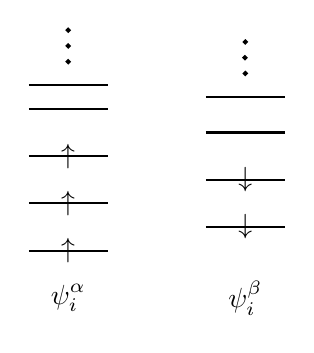
\begin{tikzpicture}[thick]
		%=========== figure left, from bottom to top===========================
		\draw (.5, -.6)node{$\displaystyle \psi_i^\alpha$};
		\draw (0,0)--++(.5,0)node{$\uparrow$}-- ++(.5,0);
		\draw (0,.6)--++(.5,0)node{$\uparrow$}-- ++(.5,0);
		\draw (0,1.2)--++(.5,0)node{$\uparrow$}-- ++(.5,0);
		\draw (0,1.8)--++(.5,0) -- ++(.5,0);
		\draw (0,2.1)--++(.5,0)-- ++(.5,0);
		\filldraw (0.5,2.4)circle(.5pt) (.5,2.6)circle(.5pt) (.5,2.8)circle(.5pt);
		%=========== figure right, from bottom to top===========================
		\draw (2.75,-.6)node{$\displaystyle \psi_i^\beta$};
		\draw (2.25,.3)--++(.5,0)node{$\downarrow$}-- ++(.5,0);
		\draw (2.25,.9)--++(.5,0)node{$\downarrow$}-- ++(.5,0);
		\draw (2.25,1.5)--++(.5,0)-- ++(.5,0);
		\draw (2.25,1.95)--++(.5,0)-- ++(.5,0);
		\filldraw (2.75,2.25)circle(.5pt) (2.745,2.45)circle(.5pt) (2.75,2.65)circle(.5pt);
	\end{tikzpicture}
\end{center}
算符$f^\alpha(1)$包含动能,
核吸引势能以及$\alpha$自旋电子感受到的有效势能。
一个$\alpha$自旋的电子所受到的有效势包括,
与其他所有$\alpha$电子的库伦和交换作用,
以及与所有$\beta$电子的库伦作用。
那么就有
\begin{align}\label{3.316}
	f^\alpha(1) = h(1) + \sum_{a}^{N^\alpha}[J_a^\alpha(1) - K_a^\alpha(1)] + \sum_{a}^{N^\beta}[J_a^\beta(1)]
\end{align}
式中第一个求和号遍及$N_\alpha$个由$\alpha$自旋电子占据的$\psi_a^\alpha$轨道,
第二个求和号遍及$N_\beta$个由$\beta$自旋电子占据的$\psi_a^\beta$轨道。
动能项和势能项与自旋无关,
因此这里的$h(1)$与限制性情形下的相同。
$\alpha$自旋的电子可以感受到库伦势$J_a^\alpha$和交换势$-K_a^\alpha$,
这两类势来自于$N_\alpha$个在$\psi_a^\alpha$轨道上的$\alpha$自旋电子。
与此同时,
还有库伦势$J_a^\beta$,
这部分来自$N_\beta=N-N_\alpha$个在$\psi_a^\beta$轨道上的$\beta$自旋电子。
上式中对$N_\alpha$个$\psi_a^\alpha$的求和包含了$\alpha$电子与它自身的相互作用。
但只要注意到
\begin{align}\label{3.317}
	[J_a^\alpha(1) - K_a^\alpha(1)]\psi_a^\alpha = 0
\end{align}
所以这个自相互作用被消除了。
带$\beta$自旋的电子对应的Fock算符为
\begin{align}\label{3.318}
	f^\beta(1) = h(1) + \sum_{a}^{N^\beta}[J_a^\beta(1) - K_a^\beta(1) ] + \sum_{a}^{N^\alpha}[J_a^\alpha(1)].
\end{align}
上面两式中的库伦与交换算符的定义与之前的定义\autoref{3.124}\autoref{3.125}类似。
写出来就是
\begin{align}
	J_a^\alpha(1) & = \int \dd\bfr_2 \psi_a^{\alpha*}(2) \twoe \psi_a^\alpha(2) \label{3.319}\\
	K_a^\alpha(1)\psi_i^\alpha(1) 
	    &= \left[ \int \dd\bfr_2 \psi_a^{\alpha*}(2) \twoe \psi_i^\alpha(2)\right] \psi_a^\alpha(1) \notag\\
	    &= \left[ \int \dd\bfr_2 \psi_a^{\alpha*}(2) \twoe \mathscr{P}_{12}\psi_a^\alpha(2)\right] \psi_i^\alpha(1) \label{3.320}
\end{align}
$J_a^\beta,K_a^\beta$的定义也完全类似。

由两个Fock算符的$f^\alpha,f^\beta$的定义\autoref{3.316}\autoref{3.318}可见,
它们对应的两个\phrase{积分-微分-本征值方程}\autoref{3.312}\autoref{3.313}无法相互独立地求解。
也即,
$f^\alpha$依赖于$\beta$占据轨道$\psi_a^\beta$,
因为$f^\alpha$中包含$J_a^\beta$。
而反过来$f^\beta$也依赖于$\alpha$占据轨道$\psi_a^\beta$,
因为$f^\beta$中包含$J_a^\alpha$。
这两个方程必须同时迭代求解。

\exercise{
	假如不用上面这种观察的办法写出$f^\alpha(1)$,
	请仿照\autoref{sec3.4.1}小节中的做法,
	利用\autoref{3.314},
	将自旋变量积掉,
	然后做一些代数运算,
	推出
	\begin{align*}
		f^\alpha(1) = h(1) + \sum_{a}^{N^\alpha}[J_a^\alpha(1) - K_a^\alpha(1)] + \sum_{a}^{N^\beta}[J_a^\beta(1)]
	\end{align*}
}

至此,
非限制性\hft 方程已经推导完毕,
我们已经能够写出非限制性轨道的能、总的非限制性能量等等。
首先定义一些项:非限制性轨道$\psi_i^\alpha$或$\psi_i^\beta$上的电子的动能与核吸引势能的期望值为
\begin{align}\label{3.321}
	h_{ii}^\alpha = (\psi_i^\alpha|h|\psi_i^\alpha)\, \text{或}\, h_{ii}^\beta = (\psi_i^\beta|h|\psi_i^\beta)
\end{align}
$\psi_i^\alpha$上一个电子与$\psi_i^\beta$上一个电子之间的库伦相互作用为
\begin{align}\label{3.322}
	J_{ij}^{\alpha\beta} = J_{ji}^{\beta\alpha} = (\psi_i^\alpha|J_{i}^\beta|\psi_i^\alpha) = (\psi_j^\beta|J_{i}^\alpha|\psi_j^\beta) = (\psi_i^\alpha\psi_i^\alpha|\psi_j^\beta\psi_j^\beta)
\end{align}
而同自旋的两个电子间的库伦相互作用为
\begin{align}\label{3.323}
	J_{i j}^{\alpha \alpha}=(\psi_{i}^{\alpha}|J_{j}^{\alpha}| \psi_{i}^{\alpha})=(\psi_{j}^{\alpha}|J_{i}^{\alpha}| \psi_{j}^{\alpha})=(\psi_{i}^{\alpha} \psi_{i}^{\alpha} | \psi_{j}^{\alpha} \psi_{j}^{\alpha})
\end{align}
以及
\begin{align}\label{3.324}
	J_{i j}^{\beta \beta}=(\psi_{i}^{\beta}|J_{j}^{\beta}| \psi_{i}^{\beta})=(\psi_{j}^{\beta}|J_{i}^{\beta}| \psi_{j}^{\beta})=(\psi_{i}^{\beta} \psi_{i}^{\beta} | \psi_{j}^{\beta} \psi_{j}^{\beta})
\end{align}
自旋平行的两个电子间的交换作用为
\begin{align}\label{3.325}
	K_{i j}^{\alpha\alpha}=(\psi_{i}^{\alpha}|K_{j}^{\alpha}| \psi_{i}^{\alpha})=(\psi_{j}^{\alpha}|K_{i}^{\alpha}| \psi_{j}^{\alpha})=(\psi_{i}^{\alpha} \psi_{j}^{\alpha} | \psi_{j}^{\alpha} \psi_{i}^{\alpha})
\end{align}
以及
\begin{align}\label{3.326}
	K_{i j}^{\beta\beta}=(\psi_{i}^{\beta}|K_{j}^{\beta}| \psi_{i}^{\beta})=(\psi_{j}^{\beta}|K_{i}^{\beta}| \psi_{j}^{\beta})=(\psi_{i}^{\beta} \psi_{j}^{\beta} | \psi_{j}^{\beta} \psi_{i}^{\beta})
\end{align}
当然,
自旋相反的电子间没有交换相互作用。


现在可以写出非限制性总电子能量,
只要写出所有的贡献项
\begin{align}
	\label{3.327}
	E_{0}=\sum_{a}^{N^{\alpha}} h_{a a}^{\alpha}+\sum_{a}^{N^{\beta}} h_{a a}^{\beta}+\frac{1}{2} \sum_{a}^{N^{\alpha}} \sum_{b}^{N^{\alpha}}\left(J_{a b}^{\alpha \alpha}-K_{a b}^{\alpha \alpha}\right)+\frac{1}{2} \sum_{a}^{N^{\beta}} \sum_{b}^{N^{\beta}}\left(J_{a b}^{\beta \beta}-K_{a b}^{\beta \beta}\right)+\sum_{a}^{N^{\alpha}} \sum_{b}^{N^{\beta}} J_{a b}^{a \beta}
\end{align}
上限为$N_\alpha$的求和遍及所有的占据轨道$\psi_a^\alpha$或$\psi_b^\alpha$. 
$\beta$自旋电子的规定也相同。 
第三项和第四项前都有因子$\frac{1}{2}$,
为消除自由求和中的双重计数。
自相互作用会消失,
因为$J_{a a}^{a \alpha}-K_{a a}^{\alpha \alpha}=J_{a a}^{\beta \beta}-K_{a a}^{\beta \beta}=0$,
正如\autoref{3.323}\autoref{3.326}中我们验证的那样。

\exercise{
	Li 原子的非限制性双重态基态为$\ket{\Psi_0} = \ket{ \psi_1^\alpha(1)\bra{\psi}_1^\beta(2 \psi_2^\alpha(3)) }$。
	请证明, 
	该态的能量为 $E_0 = h_{11}^\alpha + h_{11}^\beta + h_{22}^\alpha + J_{11}^{\alpha\alpha} - K_{12}^{\alpha\alpha} + J_{11}^{\alpha\beta} + J_{21}^{\alpha\beta}$。
	\Next
	非限制性轨道的能量为 $\epsilon_i^\alpha = (\psi_i^\alpha|f^\alpha|\psi_i^\alpha)$ 和$\epsilon^\beta = (\psi_i^\beta|f^\beta|\psi_i^\beta)$。
	请证明它们的表达式为
	\begin{align*}
		\varepsilon_{i}^{\alpha}=h_{i i}^{\alpha}+\sum_{a}^{N^{\alpha}}\left(J_{i a}^{\alpha \alpha}-K_{i a}^{\alpha \alpha}\right)+\sum_{a}^{N^{\beta}} J_{i a}^{\alpha \beta} \\
		\varepsilon_{i}^{\beta}=h_{i i}^{\beta}+\sum_{a}^{N^{\beta}}\left(J_{i a}^{\beta \beta}-K_{i a}^{\beta \beta}\right)+\sum_{a}^{N^{\alpha}} J_{i a}^{\beta \alpha}
	\end{align*}
	导出$E_0$的表达式,
	要求其中只包含轨道能量、库伦能以及交换能。
	
}
\subsection{引入基: Pople-Nesbet方程}
要求解非限制性\hft 方程\autoref{3.312}\autoref{3.313},
我们需引入一个基组(basis set),以便将这两个\phrase{积分-微分方程}转化为矩阵方程\endnote{
	J. A. Pople and R. K. Nebet, Self-consistent orbitals for radicals, \textit{J. Chem. Phys.} \textbf{22:} 571 (1954).
},
这个办法和之前推导Roothan方程时所用办法的一样。
为此,我们引入一组基$\{\phi_\mu|\mu = 1,2,\ldots,K\}$,并用这组基展开非限制性分子轨道:
\begin{align}
	\psi_i^\alpha = \sum_{\mu=1}^K C_{\mu i}^\alpha \phi_\mu \quad i =1,2,\ldots,K \label{3.328} \\
	\psi_i^\beta = \sum_{\mu=1}^K C_{\mu i}^\beta \phi_\mu \quad i =1,2,\ldots,K \label{3.329}
\end{align}
\autoref{3.312}\autoref{3.313}这两个本征值方程保证了本征函数$\{\psi_i^\alpha\}$和$\{\psi_i^\beta\}$分别构成正交归一集,
但是$\psi_i^\alpha$和$\psi_i^\beta$不一定正交。
但即使这两组空间轨道之间有重叠,$2K$个自旋轨道的集合$\{\chi_i\}$依然正交归一:
要么来自空间正交($\alpha\alpha$和$\beta\beta$的情况),
要么来自自旋正交($\alpha\beta$的情况). 

将轨道$\psi^\alpha_j$按\autoref{3.328}展开,代入$\alpha$自旋的\hft 方程\autoref{3.312},得到
\begin{align}
	\sum_\nu C^\alpha_{\nu j}f^\alpha(1)\phi_\nu(1)=\epsilon^\alpha_j\sum_\nu C^\alpha_{\nu j}\phi_\nu(1)
\end{align}
两边左乘$\phi_\mu^*(1)$并对电子1的空间坐标积分,得到
\begin{align}
	\sum_\nu F^\alpha_{\mu\nu}C^\alpha_{\nu j} = \epsilon^\alpha_j\sum_\nu S_{\mu\nu}C^\alpha_{\nu j} \quad j=1,2,\ldots,K
\end{align}
其中$\mathbf{S}$是重叠矩矩阵(\autoref{3.136}),$\mathbf{F}^\alpha$是$f^\alpha$在基组$\{\phi_\mu\}$下的矩阵表示:
\begin{align}
	F^\alpha_{\mu\nu}=\int{\dd\bfr_1}\phi^*_\mu(1)f^\alpha(1)\phi_\nu(1)
\end{align}
对$\beta$轨道也可以得到相同的结果。\autoref{3.331}和$\beta$轨道对应的方程可以写成矩阵形式:
\begin{align}
	\mathbf{F}^\alpha\mathbf{C}^\alpha = \mathbf{S}\mathbf{C}^\alpha\bm{\epsilon}^\alpha\\
	\mathbf{F}^\beta\mathbf{C}^\beta = \mathbf{S}\mathbf{C}^\beta\bm{\epsilon}^\beta
\end{align}
这两个方程是限制性Roothaan方程\autoref{3.139}的非限制性推广,由Pople和Nesbet首先给出。
$\bm{\epsilon}^\alpha$和$\bm{\epsilon}^\beta$是对角矩阵,对角元为轨道能量\autoref{3.141}. 
$K\times K$方阵$\mathbf{C}^\alpha$和$\mathbf{C}^\beta$的列是轨道$\psi_i^\alpha$和$\psi_i^\beta$的展开系数。
这两个方程可以用类似于求解Roothaan方程的方式求解,但因为$\mathbf{F}^\alpha$和$\mathbf{F}^\beta$都同时依赖$\mathbf{C}^\alpha$和$\mathbf{C}^\beta$,
所以必须同时求解这两个矩阵本征值问题。我们将在给出非限制性密度矩阵和$F^\alpha_{\mu\nu}$、$F^\beta_{\mu\nu}$的表达式后再回来求解这两个方程。
\subsection{非限制性密度矩阵}
我们从限制性闭壳层波函数的结果出发。
如果一个电子占据分子轨道$\psi_a^\alpha(\bfr)$,则在$\bfr$处的体积元$\dd\bfr$内找到该电子的概率是$|\psi^\alpha_a(\bfr)|^2\dd\bfr$,
概率分布函数(电荷密度)是$|\psi^\alpha_a(\bfr)|^2$。如果有$N^\alpha$个$\alpha$自旋的电子,则它们对总电荷密度的贡献为
\begin{align}
	\label{3.335}
	\rho^\alpha(\bfr)=\sum^{N^\alpha}_a|\psi_a^\alpha(\bfr)|^2
\end{align}
相应地,$\beta$自旋的电子贡献的电荷密度为
\begin{align}
	\label{3.336}
	\rho^\beta(\bfr)=\sum^{N^\beta}_a|\psi_a^\beta(\bfr)|^2
\end{align}
这些电子的总电荷密度是二者之和:
\begin{align}
	\rho^T(\bfr)=\rho^\alpha(\bfr)+\rho^\beta(\bfr)
\end{align}
对这个方程积分,正如预期,得到电子数:
\begin{align}
	\int{\dd\bfr}\rho^T(\bfr)=N=N^\alpha+N^\beta
\end{align}
在非限制性波函数中,$\alpha$和$\beta$自旋的电子有不同的空间分布($\rho^\alpha\neq\rho^\beta$)。
方便起见,定义\phrase{自旋密度}$\rho^S(\bfr)$
\begin{align}
	\rho^S(\bfr)=\rho^\alpha(\bfr)-\rho^\beta(\bfr)
\end{align}
根据上述定义,在找到$\alpha$自旋电子比找到$\beta$自旋电子概率更高的区域自旋密度为正,反之为负。
当然$\rho^\alpha$和$\rho^\beta$总是正的。 
自旋密度便于在开壳层体系中描述自旋分布。
\exercise{
	利用定义\autoref{3.335},\autoref{3.336}和\autoref{2.254},证明自旋密度在全空间的积分是$2\braket{\ts_z}$。
}
将$\alpha$和$\beta$分子轨道的基组展开\autoref{3.328}和\autoref{3.329}代入\autoref{3.335}和\autoref{3.336},得到$\alpha$和$\beta$电荷密度的矩阵表象(密度矩阵):
\begin{align}
	\rho^\alpha(\bfr)=\sum^{N^\alpha}_a|\psi^\alpha_a(\bfr)|^2=\sum_\mu\sum_\nu P^\alpha_{\mu\nu}\phi_\mu(\bfr)\phi_\nu^*(\bfr) \label{3.340}\\
	\rho^\beta(\bfr)=\sum^{N^\beta}_a|\psi^\beta_a(\bfr)|^2=\sum_\mu\sum_\nu P^\beta_{\mu\nu}\phi_\mu(\bfr)\phi_\nu^*(\bfr)
\end{align}
其中$\alpha$和$\beta$电子的密度矩阵$\mathbf{P}^\alpha$和$\mathbf{P}^\beta$定义为
\begin{align}
	P^\alpha_{\mu\nu}=\sum^{N^\alpha}_aC^\alpha_{\mu a}C^{\alpha*}_{\nu a} \\
	P^\beta_{\mu\nu}=\sum^{N^\beta}_aC^\beta_{\mu a}C^{\beta*}_{\nu a} \label{3.343}
\end{align}
除这两个密度矩阵外,还可以类似地定义\phrase{总密度矩阵}和\phrase{自旋密度矩阵}:
\begin{align}
	\mathbf{P}^T=\mathbf{P}^\alpha+\mathbf{P}^\beta \\
	\mathbf{P}^S=\mathbf{P}^\alpha-\mathbf{P}^\beta
\end{align}
\exercise{
	补全推导出\autoref{3.340}至\autoref{3.343}的步骤。
	\Next
	证明:自旋无关的单电子算符之和$\sum^N_{i=1}h(i)$的期待值为:
	\begin{align*}
		\braket{\mathscr{O}_1}=\sum_\mu\sum_\nu P^T_{\mu\nu}(\nu|h|\mu)
	\end{align*}
	\Next
	考虑下面的自旋相关算符,它是单电子算符之和:
	\begin{align*}
		\hat{\rho}^S=2\sum^N_{i=1}\delta(\bfr_i-\mathbf{R})s_z(i)
	\end{align*}
	利用第二章的矩阵元规则,证明$\hat{\rho}^S$对任意非限制性单行列式的期待值是
	\begin{align*}
		\braket{\hat{\rho}^S}=\rho^S(\mathbf{R})=\tr(\mathbf{P}^S\mathbf{A})
	\end{align*}
	其中
	\begin{align*}
		A_{\mu\nu}=\phi^*_\mu(\mathbf{R})\phi_\nu(\mathbf{R})
	\end{align*}
	这个矩阵元在ESR和NMR耦合常数的费米接触贡献理论中非常重要。
}
定义了非限制性密度矩阵$\mathbf{P}^\alpha$, $\mathbf{P}^\beta$, $\mathbf{P}^T$和$\mathbf{P}^S$后,
我们将用这些定义给出非限制性Fock矩阵$\mathbf{F}^\alpha$和$\mathbf{F}^\beta$的表达式。
\subsection{Fock矩阵的表达式}
为得到$\mathbf{F}^\alpha$和$\mathbf{F}^\beta$矩阵元的表达式,我们考虑两个Fock算符$f^\alpha$(\autoref{3.316})和$f^\beta$(\autoref{3.318})在基组$\{\phi_\mu\}$下的矩阵元,
并利用库伦和交换算符矩阵元\autoref{3.322}至\autoref{3.326}:
\begin{align}
	F^\alpha_{\mu\nu} &= \int{\dd\bfr_1}\phi^*_\mu(1)f^\alpha(1)\phi_\nu(1) \notag \\
	&=H^{\text{core}}_{\mu\nu}+\sum^{N^\alpha}_a[(\phi_\mu\phi_\nu|\psi^\alpha_a\psi^\alpha_a)-(\phi_\mu\psi^\alpha_a|\psi^\alpha_a\psi_\nu)]+\sum^{N^\beta}_a(\phi_\mu\phi_\nu|\psi^\beta_a\psi^\beta_a) \label{3.346} \\
	F^\beta_{\mu\nu} &= \int{\dd\bfr_1}\phi^*_\mu(1)f^\beta(1)\phi_\nu(1) \notag \\
	&=H^{\text{core}}_{\mu\nu}+\sum^{N^\beta}_a[(\phi_\mu\phi_\nu|\psi^\beta_a\psi^\beta_a)-(\phi_\mu\psi^\beta_a|\psi^\beta_a\psi_\nu)]+\sum^{N^\alpha}_a(\phi_\mu\phi_\nu|\psi^\alpha_a\psi^\alpha_a) \label{3.347}
\end{align}
然后代入$\psi^\alpha_a$和$\psi^\beta_a$的基组展开,得到
\begin{align}
	F^\alpha_{\mu\nu} &=H^{\text{core}}_{\mu\nu}+\sum_\lambda\sum_\sigma\sum^{N^\alpha}_a C^\alpha_{\lambda a}(C^\alpha_{\sigma a})^*[(\mu\nu|\sigma\lambda)-(\mu\lambda|\sigma\nu)]+\sum_\lambda\sum_\sigma\sum^{N^\beta}_a C^{\beta}_{\lambda a}(C^\beta_{\sigma a})^* (\mu\nu|\sigma\lambda) \notag \\
	&=H^{\text{core}}_{\mu\nu}+\sum_\lambda\sum_\sigma P^\alpha_{\lambda\sigma}[(\mu\nu|\sigma\lambda)-(\mu\lambda|\sigma\nu)]+\sum_\lambda\sum_\sigma P^\beta_{\lambda\sigma}(\mu\nu|\sigma\lambda) \notag \\
	&=H^{\text{core}}_{\mu\nu}+\sum_\lambda\sum_\sigma [P^T_{\lambda\sigma}(\mu\nu|\sigma\lambda)- P^\alpha_{\lambda\sigma}(\mu\lambda|\sigma\nu)] \label{3.348} \\
	F^\beta_{\mu\nu} &=H^{\text{core}}_{\mu\nu}+\sum_\lambda\sum_\sigma\sum^{N^\beta}_a  C^\beta_{\lambda a}(C^\beta_{\sigma a})^*[(\mu\nu|\sigma\lambda)-(\mu\lambda|\sigma\nu)]+\sum_\lambda\sum_\sigma\sum^{N^\alpha}_a C^{\alpha}_{\lambda a}(C^\alpha_{\sigma a})^* (\mu\nu|\sigma\lambda) \notag \\
	&=H^{\text{core}}_{\mu\nu}+\sum_\lambda\sum_\sigma P^\beta_{\lambda\sigma}[(\mu\nu|\sigma\lambda)-(\mu\lambda|\sigma\nu)]+\sum_\lambda\sum_\sigma P^\alpha_{\lambda\sigma}(\mu\nu|\sigma\lambda) \notag \\
	&=H^{\text{core}}_{\mu\nu}+\sum_\lambda\sum_\sigma [P^T_{\lambda\sigma}(\mu\nu|\sigma\lambda)- P^\beta_{\lambda\sigma}(\mu\lambda|\sigma\nu)] \label{3.349}
\end{align}
若将上面的表达式和相应的闭壳层表达式\autoref{3.154}比较,可以看到库伦项相等并依赖于总密度矩阵,区别只是这里$\alpha$和$\beta$有各自的表达式,而不像闭壳层那样有
\begin{align}
	P^\alpha_{\mu\nu}=P^\beta_{\mu\nu}=\frac{1}{2}P^T_{\mu\nu}
\end{align}
上述表达式体现了两组方程的耦合:$\mathbf{F}^\alpha$依赖$\mathbf{P}^\beta$(通过总密度矩阵$\mathbf{P}^T$),类似地,$\mathbf{F}^\beta$依赖$\mathbf{P}^\alpha$。
\subsection{非限制SCF方程的解}
求解非限制性SCF方程的流程和前述的求解Roothaan方程的流程本质上是相同的。
我们需要初猜两个密度矩阵$\mathbf{P}^\alpha$和$\mathbf{P}^\beta$(也就有了$\mathbf{P}^T$)。
一个显然的选择是令这些密度矩阵为零,使用$\mathbf{H}^\text{core}$作为$\mathbf{F}^\alpha$和$\mathbf{F}^\beta$初猜。
如果这样做,第一步迭代对$\alpha$和$\beta$自旋会得到相同的轨道,也就一个限制性的解。
但若$N^\alpha\neq N^\beta$,后续迭代中会有$\mathbf{P}^\alpha\neq\mathbf{P}^\beta$,最终会得出非限制性的解。

在每步迭代中,给定$\mathbf{P}^\alpha$和$\mathbf{P}^\beta$的近似,我们可以构建$\mathbf{F}^\alpha$和$\mathbf{F}^\beta$,然后求解两个广义矩阵本征值问题
\begin{align}
	\mathbf{F}^\alpha\mathbf{C}^\alpha = \mathbf{S}\mathbf{C}^\alpha\bm{\epsilon}^\alpha \label{3.351}\\
	\mathbf{F}^\beta\mathbf{C}^\beta = \mathbf{S}\mathbf{C}^\beta\bm{\epsilon}^\beta \label{3.352}
\end{align}
解得$\mathbf{C}^\alpha$和$\mathbf{C}^\beta$,然后构建新的近似密度矩阵$\mathbf{P}^\alpha$和$\mathbf{P}^\beta$。
因为两个方程之间的耦合,我们必须同时其自洽求解$\alpha$和$\beta$自旋的方程,即使在任意一步迭代中这两个矩阵本征值问题\autoref{3.351}和\autoref{3.352}可以独立求解。耦合出现在构造Fock矩阵的过程中。
求解矩阵本征值问题的流程和限制性闭壳层的情况一样,包括解出正交化变换矩阵$\mathbf{X}$、构造${\mathbf{F}^\alpha}'=\mathbf{X}^\dagger \mathbf{F}^\alpha\mathbf{X}$、
对角化${\mathbf{F}^\alpha}'$得到${\mathbf{C}^\alpha}'$以及$\mathbf{C}^\alpha=\mathbf{X}{\mathbf{C}^\alpha}'$。
\exercise{
	在电子能量$E_0$的表达式\autoref{3.327}中代入非限制性分子轨道的基组展开,以证明:
	\begin{align*}
		E_0=\frac{1}{2}\sum_\mu\sum_\nu[P^T_{\nu\mu}H^\text{core}_{\mu\nu}+P^\alpha_{\nu\mu}F^\alpha_{\mu\nu}+P^\beta_{\nu\mu}F^\beta_{\mu\nu}]
	\end{align*}
}
在继续讨论非限制性计算的例子之前,关于Pople-Nesbet方程的解有一个值得注意的点:在$N^\alpha=N^\beta$即闭壳层波函数可以正常描述的分子中,Pople-Nesbet方程可能有两个独立的解。
一个是限制性的解:如果$\mathbf{P}^\alpha=\mathbf{P}^\beta=\frac{1}{2}\mathbf{P}$,则$\mathbf{F}^\alpha=\mathbf{F}^\beta=\mathbf{F}$,Pople-Nesbet方程退化为Roothaan方程。
\mci{当$N^\alpha=N^\beta$时,Roothaan方程的限制性解是非限制性Pople-Nesbet方程的一个解。}这个限制性解总是存在,并且是当用$\mathbf{P}^\alpha=\mathbf{P}^\beta$作初猜时的必然结果。
对$N^\alpha=N^\beta$,除这个限制性解外还存在一个具有更低能量的非限制性解。限制性解限定了$\alpha$电子的密度等于$\beta$电子的密度,
但在特定条件下(将在本章最后一节讨论)放宽这个约束会给出一个具有更低能量的非限制性解,其中$\mathbf{P}^\alpha$不等于$\mathbf{P}^\beta$。
\mci{当$N^\alpha=N^\beta$时,Pople-Nesbet方程在特定条件下存在第二个解:非限制性解}。
要找到这第二个解,使用$\mathbf{P}^\alpha\neq\mathbf{P}^\beta$的初猜很重要,否则必然会得到限制性解。
即使用了非限制性的初猜,迭代过程仍有可能收敛到限制性解。当存在两个解时,初猜很大程度上决定了迭代会收敛到哪个解。

一般用非限制性波函数来描述$N^\alpha\neq N^\beta$的开壳层分子态,不涉及上述问题。
但若采用非限制性波函数作为解离问题的解,就像随后将要讨论的那样,两个解的可能性至关重要。
\subsection{一些非限制性的算例}


\subsection{解离问题及其非限制性解}
非限制性波函数常用来描述开壳层态,
如双重态、三重态等,
都是上一小节介绍的例子。
但是在某些特定的情形下,
有些通常被视作是闭壳层单重态的态,
却可以用非限制性波函数还可以用来描述。
比如$\hd$的基态,
通常使用限制性描述(其中电子是配对的)。
我们马上也会知道,
它确实是特定条件下唯一合适的\hft 描述。
但是,
在键长很大的情况下,
我们倾向于认为它几乎是两个独立的氢原子。
那么在对此类情形的恰当描述中,
情况应当如此:一个电子附在一个氢原子上,
另外一个电子附在另一个氢原子上,
也即两个电子的空间分布完全不同。
两个电子的这种表现和限制性波函数所描述的大不相同,
限制性波函数中,
两个电子占据完全相同的空间轨道。
因此可见,
在平衡键长下,
我们需要限制性波函数,
在大键长下,
我们需要非限制性波函数。
某种程度上,
我们是想鱼与熊掌兼得。
正如前面一小节所讨论的那样,
对于Pople-Nesbet方程来说,
当$N_\alpha=N_\beta$时可以存在两个解。
那么余下的任务就是确定,
是否确有一个非限制性的额外解,
其能量比限制性解的低。
我们会了解到,
对于正常的几何构型,
并非总存在一盒额外的非限制性解。
但若把键拉长以至于该键要发生均裂,
比如$\hd$的情况:$\hd\to \mathrm{H+H}$,
$\heh$的情况不在此列:$\heh\to \mathrm{He+H^+}$,
那么非限制性解(在大键长下)总是存在的。
非限制性解中的电子不成对,
而这正是短键时的情况。
为了明显地看出注意点,
下面来研究我们的极小基$\hd$模型。


STO-3G $\hd$的Pople-Nesbet方程可以数值求解,
方法同之前求解$\mathrm{CH_3}$、$\mathrm{N_2^+}$、$\mathrm{O_2}$的方程一样。
如果想通过迭代得到非限制性解(而不是得到限制性解),
那么一个合适的非限制性初猜是必要的。
但是,
如果不用数值方法求解Pople-Nesbet矩阵方程,
而用解析的方式来表述这个问题,
那么就能清楚地看到限制性波函数如何转变为非限制性波函数。

$\hd$的限制性波函数是由对称性确定如下的
\begin{align}
	\psi_1 &= [2(1+S_{12} )]^{-1/2}(\phi_1+\phi_2)
	\label{3.356}
	\\
	\psi_1 &= [2(1-S_{12})]^{-1/2}(\phi_1-\phi_2)
	\label{3.357}
\end{align}
由于$\hd$极小基模型只有两个基函数,
只有这两个基函数所附的系数可以变化,
又因为分子轨道设定为归一化的,
所以$\hd$极小基模型一般来说会有一个自由度。
非限制性解中,
这个自由度不能如限制性解那样用对称性来确定。
但这个自由度可以方便地按照如下方式纳入到非限制波函数中来:
将非限制性分子轨道$\psi_1,\psi_2$写成(由对称性确定的)限制性轨道的线性组合
\begin{align}
	\psi_1^\alpha &= \cos\theta \psi_1 + \sin\theta \psi_2 \\
	\psi_1^\alpha &= \cos\theta \psi_1 - \sin\theta \psi_2 
\end{align}
其中的单个自由度就是$\theta$。 
仅考虑$\theta$在$0\text{°}$和$45\text{°}$之间取值即可。
$\theta=0\text{°}$对应限制性解$\psi_a^\alpha=\psi_1^\beta=\psi_1$,
而任意非零的$\theta$对应非限制性解$\psi_a^\alpha \neq \psi_1^\beta$。
非限制性的虚轨道由下式给出:
\begin{align}
	\psi_2^\alpha &= - \sin\theta \psi_1 + \cos\theta \psi_2 \label{3.358}\\
	\psi_2^\beta &=  \sin\theta \psi_1 + \cos\theta \psi_2 \label{3.359}
\end{align}
\exercise{
	证明这组$\alpha$轨道$\{ \psi_1\alpha,\psi_2^\alpha \}$以及这组$\beta$轨道$\{ \psi_1\beta,\psi_2^\beta \}$分别构成正交归一集。
	
}

将基组展开\autoref{3.356}\autoref{3.357}带入上面的四个式子中,
就可得到非限制性分子轨道的基组展开式。
我们从现在起只考虑占据分子轨道,
它们由下式给出
\begin{align}
	\psi_1^\alpha = c_1\phi_1 + c_2\phi_2 \label{3.362}\\
	\psi_1^\beta = c_2\phi_1 + c_1\phi_2 \label{3.363}
\end{align}
其中
\begin{align}
	c_1 = [2(1+S_{12} )]^{-1/2}\cos\theta + [2(1 - S_{12} )]^{-1/2}\sin\theta\\
	c_1 = [2(1+S_{12} )]^{-1/2}\cos\theta - [2(1 - S_{12} )]^{-1/2}\sin\theta
\end{align}

通过这种把$\psi_1$和$\psi_2$混合起来的做法(即\autoref{3.358}\autoref{3.359}),
$\phi_1,\phi_2$在$\psi_1^\alpha,\psi_1^\beta$的基组展开式中的权重就可以变化,
正如\autoref{3.362}\autoref{3.363}所示。
若$\theta=0$,
这个波函数就是限制性波函数($c_1=c_2=[2(1+S_{12} )]^{-1/2}$)。
而当$\theta$从零开始增加,
此时$c_1$变大,
$c_2$变小,
或者等价地说,
$\psi_1^\alpha$中的$\phi_1$成分增加,
同时$\psi_1^\beta$中的$\phi_2$成分也增加。
假若$S_{12}=0$(正是分子键长很大时的情况),
那么$\theta$达到极限值$45\text{°}$,
$c_1=1,c_2=0$,
以及
\begin{align}
	\begin{rcases*}
		\psi_1^\alpha \equiv \phi_1\\
		\psi_1^\beta \equiv \phi_2
	\end{rcases*}\theta = 45\text{°},\quad S_{12}=0
\end{align}
这恰是我们想在双氢原子体系上看到的结果:一个$\alpha$自旋的电子在$\phi_1$上,
另外一个$\beta$自旋的电子在$\phi_2$上。









\theendnotes
